\documentclass{book}

% ====== 书名、作者与自定义命令 ======
\title{Microeconomics}
\newcommand{\booksubtitle}{A notes of Intermediate Microeconomics course}
\newcommand{\booklicense}{Creative Commons Zero 1.0 Universal}

\author{Mochiao Chen}
\newcommand{\authorsubtitle}{Beijing, China}

% 便捷命令:\booktitle \bookauthor
\makeatletter
\newcommand{\booktitle}{\@title}
\newcommand{\bookauthor}{\@author}
\makeatother

% ====== 导入导言区(宏包、几何、超链接、索引等)======
\input{preamble.tex}

\begin{document}
\frontmatter

% ---- Half Title Page ----
\newgeometry{top=1.75in,bottom=.5in}
\begin{titlepage}
\begin{flushleft}

\textbf{\fontfamily{qcs}\fontsize{48}{54}\selectfont \booktitle\\}

\par\noindent\rule{\textwidth}{4pt}\\


\begin{tikzpicture}
\shade[bottom color=lightgray,top color=white]
  (0,0) rectangle (\textwidth, 1.5)
  node[midway] {\textbf{\large \textit{\booksubtitle}}};
\end{tikzpicture}

\begin{flushright}
\Large First Edition
\end{flushright}

\vspace{\fill}

\end{flushleft}
\end{titlepage}
\restoregeometry%
% ---- End of Half Title Page ----

\thispagestyle{empty}

% ---- Title Page ----
\newgeometry{top=1.75in,bottom=.5in}
\begin{titlepage}
\begin{flushleft}

\textbf{\fontfamily{qcs}\fontsize{48}{54}\selectfont \booktitle\\}

\par\noindent\rule{\textwidth}{4pt}\\


\begin{tikzpicture}
\shade[bottom color=lightgray,top color=white]
  (0,0) rectangle (\textwidth, 1.5)
  node[midway] {\textbf{\large \textit{\booksubtitle}}};
\end{tikzpicture}

\begin{flushright}
\Large First Edition
\end{flushright}

\vspace{\fill}

\textbf{\large \bookauthor}\\[3.5pt]
\textbf{\large \textit{\authorsubtitle}}

\vspace{\fill}

% 自出版 Logo(若没有 booksvg.pdf,可暂时注释掉下面两行)
\begin{center}
\fontfamily{lmtt}\small{
Published by Mochiao Chen\\
Beijing, China\\[1em]
\textit{“Economics is not a set of answers,\\
but a way of thinking.”}\\[0.5em]
--- Paul Samuelson
}
\end{center}


\end{flushleft}
\end{titlepage}
\restoregeometry%
% ---- End of Title Page ----

\thispagestyle{empty}

% 版权页 / colophon
\begin{flushleft}
\vspace*{\fill}
This book was typeset using \LaTeX{} software.\\
\vspace{\fill}
Copyright \textcopyright{} \the\year{} \bookauthor\\
License: \booklicense%
\end{flushleft}

% 双标题页导致页码校正(保持模板逻辑)
\addtocounter{page}{2}
\chapter*{Preface}

\begin{verse}
Beneath the curve where want and wisdom meet,\\
Desire bends softly toward constraint's embrace;\\
The market hums—a silent, measured beat,\\
Where countless hearts converge in ordered grace.\\

Each price a whisper, every choice a vow,\\
The hand unseen adjusts the trembling scale;\\
From chaos born, an equilibrium now,\\
So fragile that one breath might tip the veil.\\

Yet reason builds its temples out of thought,\\
Not marble, but theorems shaped by light;\\
Each symbol holds the battles reason fought,\\
Each graph a dawn that conquered human night.\\

Thus study, patient soul, this art of cause and will—\\
Where freedom bends, yet harmony lies still.
\end{verse}

\vspace{1em}

This book of notes is primarily based on Hal R. Varian's \textit{Intermediate Microeconomics},  
and was compiled during distinguished Professor \textbf{Zhang Haiyang}'s course at the University of International Business and Economics.  
The author's understanding is limited, and omissions or errors are entirely his own responsibility.

\begin{flushright}
\textit{Mochiao Chen}\\
University of International Business and Economics\\
October 2025
\end{flushright}


% 三层目录
\setcounter{tocdepth}{3}
\tableofcontents

\mainmatter%

% ====== 逐章插入(建议每章一个文件)======
% ======================
% FILE: chapters/chap1.tex
% ======================
\chapter{The Market}\label{chap:market}

\section{Introduction}

In microeconomics, we study the behavior of individual economic agents---primarily consumers and firms---and how they interact in markets. We typically build simplified models to understand complex economic phenomena. A key principle in our modeling is the \textbf{optimization principle}, which states that people try to choose the best patterns of consumption that they can afford. Another is the \textbf{equilibrium principle}, where prices adjust until the amount that people demand of something is equal to the amount that is supplied.

In this introductory chapter, we will look at a fundamental concept for evaluating economic outcomes: efficiency. This will provide a criterion to judge how well an economic system performs.

\section{Pareto Efficiency}\label{sec:pareto}

When we want to evaluate the desirability of different economic allocations, we need a standard. One of the most widely used concepts is named after the Italian economist Vilfredo Pareto (1848--1923).

\begin{definition}[Pareto Improvement and Efficiency]
\begin{itemize}
    \item A \textbf{\index{Pareto improvement}Pareto improvement} is a change to a different allocation that makes at least one individual better off without making any other individual worse off.
    \item If an allocation allows for a Pareto improvement, it is called \textbf{\index{Pareto inefficient}Pareto inefficient}.
    \item If an allocation is such that no Pareto improvements are possible, it is called \textbf{\index{Pareto efficient}Pareto efficient}.
\end{itemize}
\end{definition}

A Pareto efficient outcome can be thought of as one with ``no wasted welfare''. That is, in a Pareto efficient allocation, the only way to improve one person's welfare is to lower another person's welfare.

\begin{remark}
    \begin{itemize}
    \item A Pareto inefficient outcome implies that there are still unrealized mutual gains-to-trade. It is possible to rearrange the allocation of goods to make someone happier without hurting anyone else.
    \item Any market outcome that achieves all possible gains-to-trade must be Pareto efficient. The concept of Pareto efficiency is a cornerstone of welfare economics.
\end{itemize}
\end{remark}
% ======================
% FILE: chapters/chap2.tex
% ======================
\chapter{Budget Constraint}\label{chap:budget}

\section{Consumption Choice Sets}

Consumers choose to consume bundles of goods and services. A \textbf{consumption bundle} is a vector of quantities of each good, e.g., $(x_1, x_2, \dots, x_n)$, where $x_i$ is the quantity of good $i$. The \textbf{consumption choice set} is the collection of all consumption bundles available to the consumer.

The choices a consumer can make are constrained by various factors, with the most prominent being the budget constraint. Other constraints can include time, resource limitations, and legal restrictions. For now, we will focus on the budgetary constraint.

\section{The Budget Constraint}

Let's consider a consumer with a disposable income of $m$ who can consume $n$ goods. The prices of these goods are given by the price vector $(p_1, p_2, \dots, p_n)$.

\begin{definition}[Affordable Consumption Bundles]
A consumption bundle $(x_1, \dots, x_n)$ is affordable if its total cost is no more than the consumer's income. That is:
\begin{equation}
    p_1x_1 + p_2x_2 + \cdots + p_n x_n \leq m
\end{equation}
This inequality is the consumer's \textbf{budget constraint}.
\end{definition}

\begin{definition}[Budget Set]
The \textbf{budget set} is the set of all affordable consumption bundles. Assuming non-negative consumption, the budget set $B$ is:
\begin{equation}
    B(p_1, \dots, p_n, m) = \{ (x_1, \dots, x_n) \mid x_i \geq 0 \text{ for all } i, \text{ and } \sum_{i=1}^{n} p_i x_i \leq m \}
\end{equation}
The upper boundary of the budget set, where the consumer spends all their income, is called the \textbf{budget line}:
\begin{equation}
    p_1x_1 + p_2x_2 + \cdots + p_n x_n = m
\end{equation}
\end{definition}

\subsection{The Two-Good Case}

For simplicity, we often analyze the case with only two goods. The budget line is then given by $p_1x_1 + p_2x_2 = m$. We can rearrange this to express $x_2$ as a function of $x_1$:
\begin{equation}
    x_2 = -\frac{p_1}{p_2}x_1 + \frac{m}{p_2}
\end{equation}
This is a linear equation.
\begin{itemize}
    \item The vertical intercept is $m/p_2$, which is the maximum amount of good 2 the consumer can buy.
    \item The horizontal intercept is $m/p_1$, which is the maximum amount of good 1 the consumer can buy.
    \item The slope is $-p_1/p_2$. The slope measures the rate at which the market is willing to ``substitute'' good 2 for good 1. It is the \textbf{opportunity cost} of consuming good 1: to consume one more unit of good 1, the consumer must give up $p_1/p_2$ units of good 2.
\end{itemize}

\begin{remark}[Graphical Representation]
The budget set for two goods is a right-angled triangle in the $(x_1, x_2)$ plane, with vertices at $(0,0)$, $(m/p_1, 0)$, and $(0, m/p_2)$. The hypotenuse of this triangle is the budget line. Bundles inside the triangle are affordable but do not exhaust income. Bundles on the budget line are just affordable. Bundles outside the triangle are unaffordable.
\end{remark}

\section{Changes in the Budget Line}

The budget set depends on prices and income. When these parameters change, the set of affordable choices changes as well.

\subsection{Income Changes}
An increase in income $m$ to $m' > m$ leads to a new budget line:
\[ x_2 = -\frac{p_1}{p_2}x_1 + \frac{m'}{p_2} \]
The slope $(-p_1/p_2)$ remains unchanged, but the vertical intercept increases. This means the budget line makes a \textbf{parallel shift outwards}. An income increase expands the budget set, meaning no original choices are lost and new choices are added. Thus, a higher income cannot make a consumer worse off. Conversely, a decrease in income shifts the budget line inward, shrinking the choice set.

\subsection{Price Changes}
Suppose the price of good 1 decreases from $p_1$ to $p_1' < p_1$. The new budget line is:
\[ x_2 = -\frac{p_1'}{p_2}x_1 + \frac{m}{p_2} \]
The vertical intercept $(m/p_2)$ is unchanged. The horizontal intercept increases to $m/p_1'$. The slope becomes flatter (less negative). The budget line \textbf{pivots outward} around the vertical intercept. Reducing the price of one commodity also expands the budget set, and thus cannot make the consumer worse off.

\section{Taxes, Subsidies, and Rationing}

\subsection{Uniform Ad Valorem Sales Tax}
An \textit{ad valorem} (from the value) sales tax is levied as a percentage of the price. If a uniform tax rate $t$ is applied to all goods, the new prices become $p_1(1+t)$ and $p_2(1+t)$. The budget constraint becomes:
\[ p_1(1+t)x_1 + p_2(1+t)x_2 = m \]
This can be rewritten as:
\[ p_1x_1 + p_2x_2 = \frac{m}{1+t} \]
A uniform sales tax is thus equivalent to a decrease in income from $m$ to $m/(1+t)$. This causes a parallel inward shift of the budget line.

\begin{examplebox}{The Food Stamp Program}
Food stamps are coupons that can be legally exchanged only for food. Let $F$ be food and $G$ be all other goods. Assume $p_F = p_G = \$1$ and income is $m=\$100$. The initial budget line is $F+G=100$.

Suppose the consumer receives \$40 worth of food stamps.
\begin{itemize}
    \item The consumer can now consume up to \$140 of food if they spend all their income on it.
    \item However, the food stamps cannot be used for other goods, so the maximum amount of other goods is still \$100.
    \item The budget constraint becomes kinked. It is $F+G=100$ for $F > 40$, but for $F \leq 40$, the consumer can still spend their full \$100 on other goods. The new budget set is larger. The budget line is:
    \[ G = \begin{cases} 100 & \text{if } 0 \leq F \leq 40 \\ 140 - F & \text{if } 40 < F \leq 140 \end{cases} \]
\end{itemize}
What if the food stamps can be traded on a black market, e.g., for \$0.50 each?
\begin{itemize}
    \item The \$40 in food stamps could be sold for $40 \times \$0.50 = \$20$.
    \item This effectively increases the consumer's cash income to $\$100 + \$20 = \$120$.
    \item The budget line would then be $F+G=120$, further expanding the budget set.
\end{itemize}
\end{examplebox}

\section{Shapes of Budget Constraints}
If prices are not constant, the budget constraint may not be a straight line.
\begin{itemize}
    \item \textbf{Quantity Discounts:} Suppose $p_1=\$2$ for the first 20 units and $p_1=\$1$ for any unit thereafter, with $p_2=\$1$ and $m=\$100$. The budget line will have a slope of $-2$ for $x_1 \leq 20$ and a slope of $-1$ for $x_1 > 20$. The budget line becomes flatter after $x_1=20$, creating a kink.
    \item \textbf{Quantity Penalties (Taxes):} The opposite occurs, and the budget line becomes steeper after a certain quantity.
    \item \textbf{One Price Negative:} If good 1 is a ``bad'' like garbage, you might be paid to accept it, i.e., $p_1 < 0$. If $p_1 = -\$2$, $p_2=\$1$ and $m=\$10$, the budget line is $-2x_1 + x_2 = 10$, or $x_2 = 2x_1 + 10$. The slope is positive, and the budget set is unbounded on the $x_1$ side.
\end{itemize}

\section{More General Choice Sets}
Choices are often constrained by more than just a budget. For example, there might be a time constraint, or a minimum consumption requirement for survival. A bundle is available only if it meets \textit{every} constraint. The final choice set is the \textbf{intersection} of all the individual constraint sets.
% ======================
% FILE: chapters/chap3.tex
% ======================
\chapter{Preferences}\label{chap:preferences}

After establishing what a consumer can afford (the budget set), we now turn to modeling what they want to consume. We do this using the concept of preferences.

\section{Consumer Preferences}
We will consider two consumption bundles, $\mathbf{x}=(x_1, x_2)$ and $\mathbf{y}=(y_1, y_2)$. The consumer can rank these bundles according to their desirability. There are three possibilities:
\begin{itemize}
    \item \textbf{Strict Preference:} The consumer strictly prefers bundle $\mathbf{x}$ to bundle $\mathbf{y}$. We write this as $\mathbf{x} \succ \mathbf{y}$.
    \item \textbf{Indifference:} The consumer is exactly as satisfied with bundle $\mathbf{x}$ as with bundle $\mathbf{y}$. We write this as $\mathbf{x} \sim \mathbf{y}$.
    \item \textbf{Weak Preference:} The consumer prefers or is indifferent between bundle $\mathbf{x}$ and bundle $\mathbf{y}$. We write this as $\mathbf{x} \succeq \mathbf{y}$.
\end{itemize}
These relations are linked. For example, if $\mathbf{x} \succeq \mathbf{y}$ and $\mathbf{y} \succeq \mathbf{x}$, then we can conclude that $\mathbf{x} \sim \mathbf{y}$. If $\mathbf{x} \succeq \mathbf{y}$ but it is \textit{not} the case that $\mathbf{y} \succeq \mathbf{x}$, then we can conclude $\mathbf{x} \succ \mathbf{y}$.

\section{Assumptions about Preferences}
To have a sensible theory of consumer choice, we need to impose some assumptions on preferences. These are often called axioms of rational choice.
\begin{itemize}
    \item \textbf{Completeness:} For any two bundles $\mathbf{x}$ and $\mathbf{y}$, the consumer can make a comparison. That is, either $\mathbf{x} \succeq \mathbf{y}$ or $\mathbf{y} \succeq \mathbf{x}$ (or both).
    \item \textbf{Reflexivity:} Any bundle $\mathbf{x}$ is at least as good as itself: $\mathbf{x} \succeq \mathbf{x}$. This is a trivial assumption.
    \item \textbf{Transitivity:} If a consumer thinks that $\mathbf{x}$ is at least as good as $\mathbf{y}$, and that $\mathbf{y}$ is at least as good as $\mathbf{z}$, then they must think that $\mathbf{x}$ is at least as good as $\mathbf{z}$. Formally: If $\mathbf{x} \succeq \mathbf{y}$ and $\mathbf{y} \succeq \mathbf{z}$, then $\mathbf{x} \succeq \mathbf{z}$.
\end{itemize}
A consumer with preferences that satisfy these three axioms is said to be \textbf{rational}.

\section{Indifference Curves}
Preferences can be represented graphically using \textbf{indifference curves}. An indifference curve is a set of all consumption bundles among which a consumer is indifferent.
\begin{itemize}
    \item The \textbf{weakly preferred set} for a bundle $\mathbf{x}'$ is the set of all bundles $\mathbf{y}$ such that $\mathbf{y} \succeq \mathbf{x}'$.
    \item The \textbf{strictly preferred set} for $\mathbf{x}'$ is the set of all bundles $\mathbf{y}$ such that $\mathbf{y} \succ \mathbf{x}'$.
\end{itemize}
A key property, derived from transitivity and the ``more is better'' assumption (monotonicity, see below), is that \textbf{indifference curves cannot intersect}. If they did, a point on the intersection would be indifferent to bundles on both curves. By transitivity, all bundles on both curves would have to be indifferent to each other, which contradicts the idea that one curve represents a higher level of preference than the other.

\section{Examples of Preferences}

\begin{itemize}
    \item \textbf{Perfect Substitutes:} If a consumer always regards units of commodities 1 and 2 as equivalent (e.g., at a one-to-one ratio), the commodities are perfect substitutes. The consumer's preference depends only on the total sum of the goods. The indifference curves are parallel straight lines.
    \item \textbf{Perfect Complements:} If a consumer always consumes commodities 1 and 2 in a fixed proportion (e.g., one-to-one, like left shoes and right shoes), the commodities are perfect complements. The indifference curves are L-shaped.
    \item \textbf{Bads:} If less of a commodity is always preferred, it is a \textbf{bad}. If good 1 is a bad and good 2 is a good, the indifference curves will be positively sloped.
    \item \textbf{Satiation:} A consumer may have a most preferred bundle, called a \textbf{satiation point} or \textbf{bliss point}. Bundles further away from this point are less preferred. The indifference curves are circles or ellipses centered on the bliss point.
\end{itemize}

\section{Well-Behaved Preferences}
We often make two further assumptions about preferences, which lead to ``well-behaved'' indifference curves.
\begin{definition}[Monotonicity]
Preferences are \textbf{monotonic} if more of any commodity is always preferred to less (holding the other commodity constant). This implies that commodities are \textbf{goods}, not bads, and that there is no satiation. Monotonicity ensures that indifference curves are negatively sloped.
\end{definition}

\begin{definition}[Convexity]
Preferences are \textbf{convex} if mixtures of bundles are (at least weakly) preferred to the bundles themselves. If $\mathbf{x} \sim \mathbf{y}$, then for any $t \in (0,1)$, the mixture bundle $\mathbf{z} = t\mathbf{x} + (1-t)\mathbf{y}$ is at least as good as $\mathbf{x}$ or $\mathbf{y}$ (i.e., $\mathbf{z} \succeq \mathbf{x}$).
\begin{itemize}
    \item \textbf{Strict convexity} holds if the mixture is always strictly preferred ($\mathbf{z} \succ \mathbf{x}$).
    \item Convexity implies that consumers prefer balanced bundles over extreme bundles. Graphically, the set of bundles weakly preferred to $\mathbf{x}$ is a convex set.
\end{itemize}
\end{definition}

\section{The Marginal Rate of Substitution (MRS)}\label{sec:mrs}
The slope of an indifference curve at a particular point is called the \textbf{marginal rate-of-substitution (MRS)}.
\begin{definition}[MRS]
The MRS measures the rate at which the consumer is just willing to substitute a small amount of good 2 for good 1, while remaining on the same indifference curve. Mathematically, it is the derivative of the indifference curve:
\[ MRS = \frac{dx_2}{dx_1} \]
\end{definition}
\begin{itemize}
    \item For monotonic preferences (goods), the MRS is negative, as the consumer must give up some of one good to get more of the other.
    \item For strictly convex preferences, the MRS becomes less negative as $x_1$ increases. This is known as a \textbf{diminishing marginal rate of substitution}. The indifference curve becomes flatter as we move to the right. This means the consumer is willing to give up less of good 2 to get an additional unit of good 1 as they consume more and more of good 1.
\end{itemize}
% ======================
% FILE: chapters/chap4.tex
% ======================
\chapter{Utility}\label{chap:utility}

In the previous chapter, we used indifference curves to describe preferences. While graphical, this can be cumbersome. A more convenient way to describe preferences is through a \textbf{utility function}.

\section{Utility Functions}

A utility function is a way of assigning a number to every possible consumption bundle such that more-preferred bundles get assigned larger numbers than less-preferred bundles.

\begin{definition}[Utility Function]
A function $U(\mathbf{x})$ represents a preference relation $\succeq$ if for any two bundles $\mathbf{x}'$ and $\mathbf{x}''$:
\begin{itemize}
    \item $\mathbf{x}' \succ \mathbf{x}'' \iff U(\mathbf{x}') > U(\mathbf{x}'')$
    \item $\mathbf{x}' \prec \mathbf{x}'' \iff U(\mathbf{x}') < U(\mathbf{x}'')$
    \item $\mathbf{x}' \sim \mathbf{x}'' \iff U(\mathbf{x}') = U(\mathbf{x}'')$
\end{itemize}
A preference relation can be represented by a continuous utility function if it is complete, reflexive, transitive, and continuous.
\end{definition}

An indifference curve consists of all bundles that have the same level of utility. The equation for an indifference curve is therefore $U(x_1, x_2) = k$ for some constant $k$.

\subsection{Ordinal Utility}
Utility is an \textbf{ordinal} concept. This means that the magnitude of the utility function is only important for ranking bundles. The absolute values, or the differences between them, do not have a specific meaning. If $U(\mathbf{x})=6$ and $U(\mathbf{y})=2$, we know $\mathbf{x}$ is preferred to $\mathbf{y}$, but we cannot say that $\mathbf{x}$ is ``three times as good'' as $\mathbf{y}$.

\subsection{Monotonic Transformations}
Because utility is ordinal, any strictly increasing transformation of a utility function will represent the same preferences. If $U(x_1, x_2)$ is a utility function representing some preferences, and $f$ is a strictly increasing function (i.e., $f'(z)>0$), then $V(x_1, x_2) = f(U(x_1, x_2))$ is a new utility function that represents the exact same preferences.

For example, if $U = x_1x_2$, then $V = {(x_1 x_2)}^{2} = x_1^{2}x_2^{2}$ and $W = \ln(x_1x_2) = \ln(x_1) + \ln(x_2)$ both represent the same preferences as $U$, because squaring (for positive numbers) and taking the natural log are both strictly increasing transformations.

\section{Examples of Utility Functions}

\begin{itemize}
    \item \textbf{Perfect Substitutes:} Preferences can be represented by a linear utility function of the form $U(x_1, x_2) = ax_1 + bx_2$. The indifference curves are lines with slope $-a/b$.
    \item \textbf{Perfect Complements:} Preferences for goods consumed in a fixed proportion (e.g., one-to-one) can be represented by a function like $U(x_1, x_2) = \min\{ax_1, bx_2\}$.
    \item \textbf{Quasi-linear Preferences:} A utility function that is linear in one good, e.g., $U(x_1, x_2) = v(x_1) + x_2$. The indifference curves are vertically shifted copies of each other.
    \item \textbf{Cobb-Douglas Preferences:} A commonly used functional form is the Cobb-Douglas utility function, $U(x_1, x_2) = x_1^a x_2^b$, where $a, b > 0$. These preferences exhibit well-behaved, convex indifference curves.
\end{itemize}

\section{Marginal Utility and MRS}

\begin{definition}[Marginal Utility]
The \textbf{marginal utility} (MU) of a good $i$ is the rate of change in total utility from consuming an infinitesimally small additional amount of good $i$, holding all other goods constant. It is the partial derivative of the utility function with respect to $x_i$:
\[ MU_i = \frac{\partial U}{\partial x_i} \]
\end{definition}

The magnitude of marginal utility depends on the specific utility function chosen and is not meaningful on its own (due to the ordinal nature of utility). However, it is useful for calculating the MRS\@.

\subsection{Deriving MRS from Utility}
Consider a small change in consumption $(dx_1, dx_2)$ that keeps the consumer on the same indifference curve. The total change in utility, $dU$, must be zero. The total differential of the utility function is:
\[ dU = \frac{\partial U}{\partial x_1}dx_1 + \frac{\partial U}{\partial x_2}dx_2 = 0 \]
\[ MU_1 dx_1 + MU_2 dx_2 = 0 \]
Rearranging this equation gives us the slope of the indifference curve:
\begin{equation}
    MRS = \frac{dx_2}{dx_1} = - \frac{\partial U / \partial x_1}{\partial U / \partial x_2} = - \frac{MU_1}{MU_2}
\end{equation}
The MRS is the ratio of the marginal utilities. This ratio is independent of any monotonic transformation of the utility function, which is a desirable property since the MRS has a real economic meaning (a psychological rate of trade-off) while the MU values do not.
% ======================
% FILE: chapters/chap5.tex
% ======================

\chapter{Choice}
\label{chap:choice}

\section{Introduction}

In the previous chapters, we modeled the consumer's constraints (the budget set) and their preferences (indifference curves and utility functions). We now put these two pieces together to analyze the consumer's choice. The fundamental assumption is that the consumer will choose the most preferred bundle from their budget set.

This is a problem of \textbf{constrained maximization}. Mathematically, the consumer's problem is to:
\begin{align*}
    \max_{x_1, x_2} \quad & U(x_1, x_2) \\
    \text{subject to} \quad & p_1x_1 + p_2x_2 \leq m \\
    & x_1 \geq 0, x_2 \geq 0
\end{align*}
In economics, this is known as the rational choice problem. The solution to this problem, the optimal consumption bundle $(x_1^*, x_2^*)$, is the consumer's \textbf{demanded bundle}.

\begin{definition}[Marshallian Demand]
The consumer's optimal choice $(x_1^*, x_2^*)$ at a given set of prices $(p_1, p_2)$ and income $m$ is called the consumer's demanded bundle. The functions that give the optimal amount of each good as a function of prices and income, $x_1^*(p_1, p_2, m)$ and $x_2^*(p_1, p_2, m)$, are called the \textbf{Marshallian demand functions}.
\end{definition}

\section{Finding the Optimal Choice}

Graphically, the optimal bundle is the point in the budget set that lies on the highest possible indifference curve.

\subsection{Interior Solutions with Well-Behaved Preferences}

For well-behaved preferences (monotonic and strictly convex), the optimal choice will typically be an \textbf{interior solution}, where the consumer purchases positive amounts of both goods ($x_1^* > 0$ and $x_2^* > 0$). In this case, the optimal bundle $(x_1^*, x_2^*)$ is characterized by two conditions:

\begin{enumerate}
    \item \textbf{The budget is exhausted.} The optimal point must lie on the budget line, not inside it. Because preferences are monotonic (more is better), any bundle inside the budget set has a more-preferred bundle to its northeast that is also affordable.
    \[ p_1x_1^* + p_2x_2^* = m \]
    \item \textbf{Tangency condition.} At the optimal point, the indifference curve is tangent to the budget line. This means their slopes are equal.
    \[ \text{Slope of Indifference Curve} = \text{Slope of Budget Line} \]
    \[ MRS = -\frac{p_1}{p_2} \]
    Since we know $MRS = -MU_1/MU_2$, the tangency condition can be rewritten as:
    \[ \frac{MU_1}{MU_2} = \frac{p_1}{p_2} \]
\end{enumerate}

This second condition has a powerful economic intuition: at the optimal choice, the rate at which the consumer is \textit{willing} to trade one good for another (the MRS) is equal to the rate at which the market \textit{allows} them to trade (the price ratio).

\begin{examplebox}{Computing Demand with Cobb-Douglas Preferences}
Let the consumer's utility function be of the Cobb-Douglas form:
\[ U(x_1, x_2) = x_1^a x_2^b \]
First, we find the marginal utilities and the MRS:
\[ MU_1 = \frac{\partial U}{\partial x_1} = ax_1^{a-1}x_2^b \]
\[ MU_2 = \frac{\partial U}{\partial x_2} = bx_1^a x_2^{b-1} \]
\[ MRS = -\frac{MU_1}{MU_2} = -\frac{ax_1^{a-1}x_2^b}{bx_1^a x_2^{b-1}} = -\frac{ax_2}{bx_1} \]
Now we apply the two conditions for an interior optimum:
\begin{enumerate}
    \item \textbf{Tangency:} $MRS = -p_1/p_2$
    \[ -\frac{ax_2^*}{bx_1^*} = -\frac{p_1}{p_2} \implies \frac{ax_2^*}{bx_1^*} = \frac{p_1}{p_2} \implies p_2x_2^* = \frac{b}{a} p_1x_1^* \]
    \item \textbf{Budget Exhaustion:} $p_1x_1^* + p_2x_2^* = m$
\end{enumerate}
Substitute the result from the tangency condition into the budget constraint:
\[ p_1x_1^* + \left(\frac{b}{a} p_1x_1^*\right) = m \]
\[ p_1x_1^* \left(1 + \frac{b}{a}\right) = m \implies p_1x_1^* \left(\frac{a+b}{a}\right) = m \]
Solving for $x_1^*$ gives the demand function for good 1:
\[ x_1^*(p_1, p_2, m) = \frac{a}{a+b} \frac{m}{p_1} \]
Substituting this back into the expression for $p_2x_2^*$ from the tangency condition gives the demand for good 2:
\[ p_2x_2^* = \frac{b}{a} p_1 \left( \frac{a}{a+b} \frac{m}{p_1} \right) = \frac{b}{a+b} m \implies x_2^*(p_1, p_2, m) = \frac{b}{a+b} \frac{m}{p_2} \]
These are the Marshallian demand functions for a consumer with Cobb-Douglas preferences. They show that the consumer spends a fixed fraction of income ($a/(a+b)$ on good 1 and $b/(a+b)$ on good 2).
\end{examplebox}


\section{Non-Tangency Solutions}

The tangency condition only holds for interior solutions with smooth indifference curves. In other cases, the optimal choice may occur where the tangency condition is not met.

\subsection{Corner Solutions}
A \textbf{corner solution} occurs when the optimal quantity of one of the goods is zero. This often happens with perfect substitutes or non-convex preferences.

\begin{examplebox}{Optimal Choice with Perfect Substitutes}
Consider the utility function $U(x_1, x_2) = x_1 + x_2$. Here, the MRS is constant at $-1$. The indifference curves are straight lines with a slope of $-1$. The consumer will compare their personal trade-off rate (1-for-1) with the market's trade-off rate ($p_1/p_2$).
\begin{itemize}
    \item If $p_1 < p_2$, the slope of the budget line ($-p_1/p_2$) is flatter than the slope of the indifference curves ($-1$). The consumer gets more utility per dollar from good 1. The optimal choice is to spend all income on good 1. This is a corner solution at $(m/p_1, 0)$.
    \item If $p_1 > p_2$, the budget line is steeper than the indifference curves. The consumer gets more utility per dollar from good 2 and will spend all income on it. The corner solution is at $(0, m/p_2)$.
    \item If $p_1 = p_2$, the budget line and indifference curves have the same slope. Any affordable bundle on the budget line is an optimal choice.
\end{itemize}
So, the demand for good 1 is:
\[ x_1^*(p_1, p_2, m) = \begin{cases} m/p_1 & \text{if } p_1 < p_2 \\ \text{any amount in } [0, m/p_1] & \text{if } p_1 = p_2 \\ 0 & \text{if } p_1 > p_2 \end{cases} \]
\end{examplebox}

\subsection{Kinky Solutions}
If indifference curves have kinks, such as with perfect complements, the MRS is not well-defined at the optimal point, and the tangency condition cannot be used.

\begin{examplebox}{Optimal Choice with Perfect Complements}
Consider the utility function $U(x_1, x_2) = \min\{x_1, x_2\}$. The consumer always wants to consume the goods in a one-to-one ratio. The optimal choice will always be at the corner of an L-shaped indifference curve, where $x_1 = x_2$.
\begin{enumerate}
    \item \textbf{Consumption in fixed proportion:} $x_1^* = x_2^*$
    \item \textbf{Budget Exhaustion:} $p_1x_1^* + p_2x_2^* = m$
\end{enumerate}
Substituting the first condition into the second gives:
\[ p_1x_1^* + p_2x_1^* = m \implies (p_1+p_2)x_1^* = m \]
Solving gives the demand functions:
\[ x_1^*(p_1, p_2, m) = x_2^*(p_1, p_2, m) = \frac{m}{p_1+p_2} \]
\end{examplebox}
% ======================
% FILE: chapters/chap6.tex
% ======================

\chapter{Demand}\label{chap:demand}

\section{Introduction}

The demand functions derived in the previous chapter, $x_i^*(p_1, p_2, m)$, tell us the optimal quantities of each good as a function of prices and income. In this chapter, we explore how the quantity demanded changes as these variables change. This is known as \textbf{comparative statics}.

\section{Own-Price Changes}

We first analyze how the demand for a good, say good 1, changes as its own price, $p_1$, changes, while holding $p_2$ and income $m$ constant.

\begin{definition}[Price Offer Curve and Demand Curve]
~
\begin{itemize}
    \item The set of optimal bundles traced out as $p_1$ changes is called the \textbf{$p_1$-price offer curve} or simply the \textbf{price offer curve}.
    \item A plot of the optimal quantity demanded of good 1, $x_1^*$, against its own price, $p_1$, is the \textbf{demand curve} for good 1.
\end{itemize}
\end{definition}

\begin{definition}[Ordinary and Giffen Goods]
~
\begin{itemize}
    \item A good is called an \textbf{ordinary good} if the quantity demanded for it always increases as its own price decreases. Ordinary goods have downward-sloping demand curves.
    \item A good is called a \textbf{Giffen good} if, for some range of prices, the quantity demanded rises as its own-price increases. Giffen goods have a segment of their demand curve that is upward-sloping. They are a theoretical curiosity and are rarely observed in reality.
\end{itemize}
\end{definition}

\subsection{The Inverse Demand Function}
The standard demand curve plots quantity as a function of price, $x_1 = x_1^*(p_1)$. Sometimes it is useful to ask the inverse question: at what price would a given quantity be demanded? This gives the \textbf{inverse demand function}, which plots price as a function of quantity, $p_1 = p_1(x_1)$.

\begin{examplebox}{Cobb-Douglas Inverse Demand}
The ordinary demand function for good 1 is $x_1^* = \frac{a}{a+b}\frac{m}{p_1}$.
To find the inverse demand function, we solve for $p_1$:
\[ p_1(x_1^*) = \frac{a}{a+b}\frac{m}{x_1^*} \]
\end{examplebox}

\section{Income Changes}
We now analyze how the demand for a good changes as income $m$ changes, holding prices $(p_1, p_2)$ constant.

\begin{definition}[Income Offer Curve and Engel Curve]
~
\begin{itemize}
    \item The set of optimal bundles traced out as income $m$ changes is called the \textbf{income offer curve} or \textbf{income expansion path}.
    \item A plot of the quantity demanded of a good against income is called an \textbf{Engel curve}.
\end{itemize}
\end{definition}

\begin{definition}[Normal and Inferior Goods]
~
\begin{itemize}
    \item A good is a \textbf{normal good} if the quantity demanded rises with income ($\partial x_i^*/\partial m > 0$). A normal good has a positively sloped Engel curve.
    \item A good is an \textbf{inferior good} if the quantity demanded falls as income increases ($\partial x_i^*/\partial m < 0$). An inferior good has a negatively sloped Engel curve.
\end{itemize}
\end{definition}

\subsection{Homothetic Preferences}
An important class of preferences are those that are \textbf{homothetic}. For these preferences, the MRS depends only on the ratio of the goods, not on the scale.
\begin{proposition}
If a consumer has homothetic preferences, then their income offer curve is a straight line through the origin, and their Engel curves are straight lines.
\end{proposition}
This implies that the consumer will always spend a fixed proportion of their income on each good. Cobb-Douglas, perfect substitutes, and perfect complements are all examples of homothetic preferences.

\subsection{Non-homothetic Preferences: Quasi-linear Utility}
Quasi-linear preferences of the form $U(x_1, x_2) = v(x_1) + x_2$ are a key example of non-homothetic preferences. For these preferences, an increase in income (once it is sufficiently high) does not change the demand for good 1 at all; all extra income is spent on good 2. This results in a vertical income offer curve and a vertical Engel curve for good 1 above a certain income level.

\section{Cross-Price Effects}

Finally, we consider how the demand for good 1 changes when the price of \textit{another} good, $p_2$, changes.

\begin{definition}[Gross Substitutes and Complements]
~
\begin{itemize}
    \item Good 1 is a \textbf{gross substitute} for good 2 if an increase in $p_2$ increases the demand for good 1 ($\partial x_1^*/\partial p_2 > 0$).
    \item Good 1 is a \textbf{gross complement} for good 2 if an increase in $p_2$ reduces the demand for good 1 ($\partial x_1^*/\partial p_2 < 0$).
\end{itemize}
\end{definition}

\begin{examplebox}{Cross-Price Effects Examples}
~
\begin{itemize}
    \item \textbf{Perfect Complements:} $x_1^* = m/(p_1+p_2)$. Taking the derivative:
    \[ \frac{\partial x_1^*}{\partial p_2} = -\frac{m}{(p_1+p_2)^2} < 0 \]
    As expected, the goods are gross complements.
    \item \textbf{Cobb-Douglas:} $x_1^* = \frac{a}{a+b}\frac{m}{p_1}$. Taking the derivative:
    \[ \frac{\partial x_1^*}{\partial p_2} = 0 \]
    In the Cobb-Douglas case, the demand for one good is independent of the other good's price. The goods are neither gross substitutes nor gross complements.
\end{itemize}
\end{examplebox}
\chapter{Revealed Preference}\label{chap:revealed_preference}

In previous chapters, we started with a consumer's preferences (or utility function) and used this information to derive their optimal choices. This chapter reverses the process. We ask: can we start by observing a consumer's choices at different prices and income levels, and from these observations, deduce their underlying preferences? This is the central question of revealed preference theory.

\section{The Concept of Revealed Preference}

The basic idea is simple yet powerful: a consumer's choice \textit{reveals} information about their preferences. If a consumer chooses a bundle of goods \(x\) when another bundle \(y\) was also affordable, we can infer that the consumer prefers \(x\) to \(y\).

\subsection{Maintained Assumptions}
To make this inference robust, we rely on a few standard assumptions about consumer behavior:
\begin{itemize}
    \item \textbf{Stable Preferences:} The consumer's preferences do not change during the period of observation.
    \item \textbf{Well-Behaved Preferences:} We assume preferences are monotonic (more is better) and strictly convex. A key implication of strict convexity is that for any given budget, there is a \textit{unique} most-preferred affordable bundle.
    \item \textbf{Rationality:} The consumer always chooses the most preferred bundle they can afford.
\end{itemize}

\subsection{Direct and Indirect Revelation}

\begin{definition}[Directly Revealed Preferred]
    Let \(\mathbf{x} = (x_1, x_2)\) be the bundle chosen at prices \(\mathbf{p} = (p_1, p_2)\), and let \(\mathbf{y} = (y_1, y_2)\) be another bundle. If \(\mathbf{y}\) was affordable at prices \(\mathbf{p}\) when \(\mathbf{x}\) was chosen, i.e., \(p_1 x_1 + p_2 x_2 \geq p_1 y_1 + p_2 y_2\), and \(\mathbf{x} \neq \mathbf{y}\), then we say that \textbf{\(\mathbf{x}\) is directly revealed preferred to \(\mathbf{y}\)}. We denote this by \(\mathbf{x} \succ_D \mathbf{y}\).
\end{definition}

The logic is that since the consumer could have chosen \(\mathbf{y}\) but instead chose \(\mathbf{x}\), they must prefer \(\mathbf{x}\).

We can extend this idea through transitivity.

\begin{definition}[Indirectly Revealed Preferred]
    If we have a chain of direct revelations, such as \(\mathbf{x} \succ_D \mathbf{y}\) and \(\mathbf{y} \succ_D \mathbf{z}\), then we say that \textbf{\(\mathbf{x}\) is indirectly revealed preferred to \(\mathbf{z}\)}. We denote this by \(\mathbf{x} \succ_I \mathbf{z}\).
\end{definition}

This allows us to compare bundles that were not available in the same budget set, by linking them through intermediate choices.

\section{Axioms of Revealed Preference}
For observed choices to be consistent with our model of a rational, utility-maximizing consumer, they must satisfy certain consistency conditions. These are known as the axioms of revealed preference.

\subsection{The Weak Axiom of Revealed Preference (WARP)}
WARP is the most basic consistency check. It ensures that if a consumer reveals a preference for one bundle over another, they don't subsequently reveal the opposite preference.

\begin{definition}[Weak Axiom of Revealed Preference (WARP)]
    If a bundle \(\mathbf{x}\) is directly revealed preferred to a bundle \(\mathbf{y}\) (\(\mathbf{x} \succ_D \mathbf{y}\)), then it can never be the case that \(\mathbf{y}\) is directly revealed preferred to \(\mathbf{x}\) (\(\mathbf{y} \succ_D \mathbf{x}\)).
    \[
    \text{If } \mathbf{x} \succ_D \mathbf{y}, \text{ then it cannot be that } \mathbf{y} \succ_D \mathbf{x}.
    \]
\end{definition}

Choice data that violate WARP are inconsistent with the model of economic rationality. WARP is a \textit{necessary} condition for choices to be rationalized by a utility function.

\begin{examplebox}{Checking for WARP Violations}
A consumer makes the following choices:
\begin{itemize}
    \item At prices \(\mathbf{p}^A = (\$2, \$2)\), the choice is \(\mathbf{x}^A = (10, 1)\).
    \item At prices \(\mathbf{p}^B = (\$2, \$1)\), the choice is \(\mathbf{x}^B = (5, 5)\).
    \item At prices \(\mathbf{p}^C = (\$1, \$2)\), the choice is \(\mathbf{x}^C = (5, 4)\).
\end{itemize}
To check for WARP violations, we calculate the cost of each bundle at each set of prices. The chosen bundle's cost represents the consumer's income in that situation.

\begin{center}
\begin{tabular}{l|ccc}
\hline
\textbf{Prices} & \textbf{Cost of \(\mathbf{x}^A\)} & \textbf{Cost of \(\mathbf{x}^B\)} & \textbf{Cost of \(\mathbf{x}^C\)} \\
\hline
\(\mathbf{p}^A = (\$2, \$2)\) & \textbf{\$22} & \$20 & \$18 \\
\(\mathbf{p}^B = (\$2, \$1)\) & \$21 & \textbf{\$15} & \$14 \\
\(\mathbf{p}^C = (\$1, \$2)\) & \$12 & \$15 & \textbf{\$13} \\
\hline
\end{tabular}
\end{center}

Let's analyze the choices:
\begin{itemize}
    \item At prices \(\mathbf{p}^A\), income is \$22. Both \(\mathbf{x}^B\) (\$20) and \(\mathbf{x}^C\) (\$18) were affordable. Thus, \(\mathbf{x}^A \succ_D \mathbf{x}^B\) and \(\mathbf{x}^A \succ_D \mathbf{x}^C\).
    \item At prices \(\mathbf{p}^B\), income is \$15. \(\mathbf{x}^C\) (\$14) was affordable. Thus, \(\mathbf{x}^B \succ_D \mathbf{x}^C\).
    \item At prices \(\mathbf{p}^C\), income is \$13. \(\mathbf{x}^A\) (\$12) was affordable. Thus, \(\mathbf{x}^C \succ_D \mathbf{x}^A\).
\end{itemize}
We have found that \(\mathbf{x}^A \succ_D \mathbf{x}^C\) and \(\mathbf{x}^C \succ_D \mathbf{x}^A\). This is a direct violation of WARP. These data are not consistent with a rational consumer.
\end{examplebox}

\subsection{The Strong Axiom of Revealed Preference (SARP)}
WARP is not sufficient to guarantee that choices can be described by a well-behaved utility function. We need a stronger condition that also rules out cycles in \textit{indirect} revealed preferences.

\begin{definition}[Strong Axiom of Revealed Preference (SARP)]
    If a bundle \(\mathbf{x}\) is revealed preferred (directly or indirectly) to a bundle \(\mathbf{y}\) (\(\mathbf{x} \succ_D \mathbf{y}\) or \(\mathbf{x} \succ_I \mathbf{y}\)), and \(\mathbf{x} \neq \mathbf{y}\), then it can never be the case that \(\mathbf{y}\) is revealed preferred (directly or indirectly) to \(\mathbf{x}\).
\end{definition}

SARP is the key condition. It has been proven that if a finite set of observed choices satisfies SARP, then there exists a well-behaved (monotonic, convex) preference relation that ``rationalizes'' these choices. Thus, SARP is both a \textit{necessary and sufficient} condition for the data to be consistent with the standard economic model of consumer choice.

\begin{examplebox}{A SARP Violation (with no WARP violation)}
Consider the following data:
\begin{itemize}
    \item Prices \(\mathbf{p}^A=(1,3,10)\), Choice \(\mathbf{x}^A=(3,1,4)\).
    \item Prices \(\mathbf{p}^B=(4,3,6)\), Choice \(\mathbf{x}^B=(2,5,3)\).
    \item Prices \(\mathbf{p}^C=(1,1,5)\), Choice \(\mathbf{x}^C=(4,4,3)\).
\end{itemize}
\begin{center}
\begin{tabular}{l|ccc}
\hline
\textbf{Prices} & \textbf{Cost of \(\mathbf{x}^A\)} & \textbf{Cost of \(\mathbf{x}^B\)} & \textbf{Cost of \(\mathbf{x}^C\)} \\
\hline
\(\mathbf{p}^A = (1,3,10)\) & \textbf{\$46} & \$47 & \$46 \\
\(\mathbf{p}^B = (4,3,6)\) & \$39 & \textbf{\$41} & \$46 \\
\(\mathbf{p}^C = (1,1,5)\) & \$24 & \$22 & \textbf{\$23} \\
\hline
\end{tabular}
\end{center}
Let's analyze the direct revelations:
\begin{itemize}
    \item At prices \(\mathbf{p}^A\), \(\mathbf{x}^C\) was affordable (\(\$46 \leq \$46\)). So, \(\mathbf{x}^A \succ_D \mathbf{x}^C\).
    \item At prices \(\mathbf{p}^B\), \(\mathbf{x}^A\) was affordable (\(\$39 \leq \$41\)). So, \(\mathbf{x}^B \succ_D \mathbf{x}^A\).
    \item At prices \(\mathbf{p}^C\), \(\mathbf{x}^B\) was affordable (\(\$22 \leq \$23\)). So, \(\mathbf{x}^C \succ_D \mathbf{x}^B\).
\end{itemize}
This dataset does not violate WARP (check: no pairs like \(X \succ_D Y\) and \(Y \succ_D X\)). However, let's look at the indirect revelations. We have a cycle:
\[
\mathbf{x}^B \succ_D \mathbf{x}^A \quad \text{and} \quad \mathbf{x}^A \succ_D \mathbf{x}^C \implies \mathbf{x}^B \succ_I \mathbf{x}^C
\]
But we also found that \(\mathbf{x}^C \succ_D \mathbf{x}^B\). This is a violation of SARP. These choices cannot be rationalized by a well-behaved preference relation.
\end{examplebox}

\section{Applications of Revealed Preference}
The theory of revealed preference provides the foundation for practical economic tools, such as index numbers, which are used to measure changes in welfare and the cost of living.

\subsection{Index Numbers and Welfare}
Index numbers compare expenditures in a base period (b) and a current period (t). Let \(\mathbf{p}^b, \mathbf{x}^b\) be the prices and chosen bundle in the base period, and \(\mathbf{p}^t, \mathbf{x}^t\) be for the current period.

\subsubsection{Quantity Indices}
A quantity index measures the change in consumption levels, holding prices constant.
\begin{itemize}
    \item The \textbf{Laspeyres Quantity Index} uses base period prices as weights:
    \[
    L_q = \frac{\mathbf{p}^b \cdot \mathbf{x}^t}{\mathbf{p}^b \cdot \mathbf{x}^b} = \frac{p_1^b x_1^t + p_2^b x_2^t}{p_1^b x_1^b + p_2^b x_2^b}
    \]
    If \(L_q < 1\), it means \(\mathbf{p}^b \cdot \mathbf{x}^b > \mathbf{p}^b \cdot \mathbf{x}^t\). At base period prices, the consumer chose \(\mathbf{x}^b\) when \(\mathbf{x}^t\) was affordable. By revealed preference, the consumer was better off in the base period b.

    \item The \textbf{Paasche Quantity Index} uses current period prices as weights:
    \[
    P_q = \frac{\mathbf{p}^t \cdot \mathbf{x}^t}{\mathbf{p}^t \cdot \mathbf{x}^b} = \frac{p_1^t x_1^t + p_2^t x_2^t}{p_1^t x_1^b + p_2^t x_2^b}
    \]
    If \(P_q > 1\), it means \(\mathbf{p}^t \cdot \mathbf{x}^t > \mathbf{p}^t \cdot \mathbf{x}^b\). At current period prices, the consumer chose \(\mathbf{x}^t\) when \(\mathbf{x}^b\) was affordable. The consumer is better off in the current period t.
\end{itemize}

\subsubsection{Price Indices}
A price index measures the change in prices, holding quantities constant.
\begin{itemize}
    \item The \textbf{Laspeyres Price Index} uses the base period bundle as weights:
    \[
    L_p = \frac{\mathbf{p}^t \cdot \mathbf{x}^b}{\mathbf{p}^b \cdot \mathbf{x}^b} = \frac{p_1^t x_1^b + p_2^t x_2^b}{p_1^b x_1^b + p_2^b x_2^b}
    \]
    \item The \textbf{Paasche Price Index} uses the current period bundle as weights:
    \[
    P_p = \frac{\mathbf{p}^t \cdot \mathbf{x}^t}{\mathbf{p}^b \cdot \mathbf{x}^t} = \frac{p_1^t x_1^t + p_2^t x_2^t}{p_1^b x_1^t + p_2^b x_2^t}
    \]
\end{itemize}
Let \(M = \frac{\mathbf{p}^t \cdot \mathbf{x}^t}{\mathbf{p}^b \cdot \mathbf{x}^b}\) be the ratio of total expenditure. If \(L_p < M\), it can be shown this implies \(\mathbf{p}^t \cdot \mathbf{x}^t > \mathbf{p}^t \cdot \mathbf{x}^b\), meaning the consumer is better off in the current period.

\subsection{Application: Indexation}
Price indices like the Consumer Price Index (CPI), which is a type of Laspeyres price index, are often used to adjust wages or benefits for inflation. This is called \textbf{indexation}. If an individual's income is adjusted by the full amount of the Laspeyres price index, they are typically made \textit{strictly better off}.

Why? Full indexation gives the consumer enough income (\(m' = \mathbf{p}^t \cdot \mathbf{x}^b\)) to buy their \textit{old} base-period bundle \(\mathbf{x}^b\) at the \textit{new} current-period prices \(\mathbf{p}^t\). However, since relative prices have likely changed, the consumer can usually improve their welfare by substituting away from goods that have become relatively more expensive. They will choose a new bundle \(\mathbf{x}^t\) on their new budget line. Since the old bundle \(\mathbf{x}^b\) is still affordable, but a different bundle \(\mathbf{x}^t\) is chosen, it must be that \(\mathbf{x}^t\) is revealed preferred to \(\mathbf{x}^b\). Thus, full indexation tends to overcompensate for price changes.
\chapter{Slutsky Equation}\label{chap:slutsky}

When the price of a good changes, the consumer's optimal choice is affected. This overall change in demand can be decomposed into two distinct effects. Understanding this decomposition is crucial for analyzing consumer behavior. The Slutsky equation provides a formal framework for this analysis.

\section{Effects of a Price Change}
What happens when a commodity's price decreases? The total change in the quantity demanded arises from two separate phenomena:

\begin{itemize}
    \item \textbf{Substitution Effect:} The commodity becomes relatively cheaper compared to other goods. A rational consumer will substitute towards the cheaper good, away from the now relatively more expensive ones. This effect captures the change in demand due to the change in the rate of exchange between two goods.

    \item \textbf{Income Effect:} The consumer's purchasing power increases. With the same nominal income, say \$m, the consumer can now afford to buy more goods than before. It is as if the consumer's real income has risen. This change in purchasing power leads to a change in quantity demanded, which we call the income effect.
\end{itemize}

Let's visualize this. Consider a consumer with income \(m\) facing prices \(p_1\) and \(p_2\). The budget line is \(p_1 x_1 + p_2 x_2 = m\). If the price of good 1 falls to \(p_1' < p_1\), the budget line pivots outwards around the vertical intercept (\(m/p_2\)). The consumer can now reach a higher indifference curve, representing a new optimal bundle.

The core idea behind the Slutsky equation is to separate this pivot into two conceptual steps: a pivot and a shift. To isolate the substitution effect, we need to hold the consumer's purchasing power constant.

\subsection{Slutsky Compensation}
How do we hold purchasing power constant? Slutsky's clever idea was to define it as the ability to purchase the \textit{original bundle} of goods.

\begin{definition}[Slutsky Compensation]
    The \textbf{Slutsky compensation} is the hypothetical adjustment to a consumer's income such that, at the new prices, they can \textit{just} afford their original consumption bundle. This adjusted income level keeps the consumer's purchasing power constant in the sense that the original choice remains affordable.
\end{definition}

If the original bundle was \((x_1^*, x_2^*)\) at prices \((p_1, p_2)\), and the price of good 1 changes to \(p_1'\), the compensated income \(m'\) would be:
\[
m' = p_1' x_1^* + p_2 x_2^*
\]
The change in income required for this compensation is:
\[
\Delta m = m' - m = (p_1' x_1^* + p_2 x_2^*) - (p_1 x_1^* + p_2 x_2^*) = (p_1' - p_1)x_1^* = \Delta p_1 x_1^*
\]

\section{Decomposing the Total Effect}

Let's trace the full decomposition graphically.
Let the initial optimal choice be bundle A = \((x_1^*, x_2^*)\) at prices \((p_1, p_2)\) and income \(m\).
Now, let the price of good 1 fall to \(p_1'\). The final optimal choice is bundle C = \((x_1'', x_2'')\) at prices \((p_1', p_2)\) and income \(m\). The total change in demand for good 1 is \(\Delta x_1 = x_1'' - x_1^*\).

\subsection{The Substitution Effect}
To isolate the substitution effect, we give the consumer the compensated income \(m' = p_1' x_1^* + p_2 x_2^*\). The new (compensated) budget line is \(p_1' x_1 + p_2 x_2 = m'\). Notice that this line has the slope of the \textit{new} price ratio but passes through the \textit{original} bundle A.

The consumer chooses a new optimal bundle on this compensated budget line, let's call it B = \((x_1^s, x_2^s)\).
The \textbf{Slutsky substitution effect} is the change in demand from A to B\@:
\[
\Delta x_1^s = x_1^s - x_1^*
\]

\begin{proposition}[Sign of the Substitution Effect]
The Slutsky substitution effect is always negative (or non-positive). That is, the change in quantity demanded due to the substitution effect is always in the opposite direction to the change in price. If price falls (\(\Delta p_1 < 0\)), the substitution effect on demand will be positive (\(\Delta x_1^s \ge 0\)).
\end{proposition}

\begin{proof}[Justification via WARP]
At the original prices \((p_1, p_2)\), bundle A was chosen over bundle B (since B was not affordable, assuming B is not A). At the compensated budget with prices \((p_1', p_2)\), bundle B is chosen. Bundle A is also affordable on this line by construction. Therefore, B is revealed preferred to A. If we consider a price increase from \(p_1'\) to \(p_1\), B is chosen at \(p_1'\) and A is chosen at \(p_1\). Since A was affordable at the prices where B was chosen, WARP is not violated. Crucially, the optimal bundle B on the compensated budget line must lie to the right of A if \(p_1' < p_1\), meaning \(x_1^s \ge x_1^*\).
\end{proof}

\subsection{The Income Effect}
The substitution effect is a hypothetical construct. The consumer's actual income is still \(m\), not \(m'\). The second part of the decomposition is to restore the consumer's original income, which means moving from the compensated budget line back to the final budget line. This is a parallel shift, representing a change in income from \(m'\) to \(m\).

The \textbf{income effect} is the change in demand from the intermediate bundle B to the final bundle C:
\[
\Delta x_1^n = x_1'' - x_1^s
\]
This change is purely due to the change in purchasing power, as prices are held constant at \((p_1', p_2)\) during this step.

The overall change in demand is the sum of these two effects:
\[
\text{Total Effect} = \text{Substitution Effect} + \text{Income Effect}
\]
\[
(x_1'' - x_1^*) = (x_1^s - x_1^*) + (x_1'' - x_1^s)
\]

\section{Slutsky's Effects for Different Types of Goods}

The sign of the income effect depends on whether the good is normal or inferior. This determines how the two effects combine. Let's assume a price \textbf{decrease} for good 1 (\(p_1 \downarrow\)).

\subsection{Normal Goods}
A good is \textbf{normal} if demand increases as income increases (\(\frac{\partial x_1}{\partial m} > 0\)).
\begin{itemize}
    \item \textbf{Substitution Effect:} Price falls, so demand increases (\(\Delta x_1^s > 0\)).
    \item \textbf{Income Effect:} Price falls, real income rises. Since the good is normal, demand increases (\(\Delta x_1^n > 0\)).
\end{itemize}
For a normal good, the substitution and income effects \textbf{reinforce} each other. A price decrease unambiguously leads to an increase in quantity demanded. Therefore, the Law of Demand always holds for normal goods.

\subsection{Income-Inferior Goods}
A good is \textbf{inferior} if demand decreases as income increases (\(\frac{\partial x_1}{\partial m} < 0\)).
\begin{itemize}
    \item \textbf{Substitution Effect:} Price falls, so demand increases (\(\Delta x_1^s > 0\)).
    \item \textbf{Income Effect:} Price falls, real income rises. Since the good is inferior, demand decreases (\(\Delta x_1^n < 0\)).
\end{itemize}
For an income-inferior good, the substitution and income effects \textbf{oppose} each other. The total effect depends on which effect is stronger. In most cases, the substitution effect outweighs the income effect, so a price decrease still leads to an increase in total demand.

\subsection{Giffen Goods}
In rare cases of extreme income-inferiority, the income effect can be stronger than the substitution effect.
\begin{definition}[Giffen Good]
A \textbf{Giffen good} is a good for which a decrease in price causes the quantity demanded to fall. This happens when the good is so strongly inferior that the negative income effect outweighs the positive substitution effect.
\end{definition}
For a Giffen good, the demand curve is upward-sloping. It is a violation of the Law of Demand. Slutsky's decomposition provides the theoretical explanation for this phenomenon.

\section{The Slutsky Identity}
We can express the decomposition mathematically. The total change in demand for good 1, \(\Delta x_1\), when its price changes from \(p_1\) to \(p_1'\) is:
\[
\Delta x_1 = x_1(p_1', m) - x_1(p_1, m)
\]
We can add and subtract the term \(x_1(p_1', m')\), where \(m' = p_1' x_1(p_1, m) + p_2 x_2(p_1, m)\):
\[
\Delta x_1 = \underbrace{[x_1(p_1', m') - x_1(p_1, m)]}_{\text{Substitution Effect, } \Delta x_1^s} + \underbrace{[x_1(p_1', m) - x_1(p_1', m')]}_{\text{Income Effect, } \Delta x_1^n}
\]
This is the \textbf{Slutsky identity}.

To express this in terms of rates of change, we divide by \(\Delta p_1\):
\[
\frac{\Delta x_1}{\Delta p_1} = \frac{\Delta x_1^s}{\Delta p_1} + \frac{\Delta x_1^n}{\Delta p_1}
\]
Let's analyze the income effect term. We know \(\Delta m = \Delta p_1 x_1\). Also, \(\Delta x_1^n = x_1(p_1', m) - x_1(p_1', m')\). Notice that income changes from \(m'\) to \(m\), so \(\Delta m = m - m'\).
Therefore, we can write:
\[
\frac{\Delta x_1^n}{\Delta p_1} = \frac{x_1(p_1', m) - x_1(p_1', m')}{\Delta p_1} = \frac{x_1(p_1', m) - x_1(p_1', m')}{m - m'} \frac{m - m'}{\Delta p_1} = -\frac{\Delta x_1^n}{\Delta m} x_1
\]
(The minus sign appears because \(\Delta x_1^n\) as defined is for an income change from \(m'\) to \(m\), while \(\Delta m\) from our compensation formula was \(m' - m\)).
Substituting this back gives the \textbf{Slutsky Equation}:

\begin{tcolorbox}[colback=blue!5!white, colframe=blue!75!black, fonttitle=\bfseries, title=The Slutsky Equation]
The relationship between the total effect, substitution effect, and income effect is given by:
\[
\frac{\Delta x_1}{\Delta p_1} = \frac{\Delta x_1^s}{\Delta p_1} - \frac{\Delta x_1}{\Delta m} x_1
\]
Or in calculus terms:
\[
\frac{\partial x_1(p_1, m)}{\partial p_1} = \frac{\partial x_1^s(p_1, \bar{u})}{\partial p_1} - \frac{\partial x_1(p_1, m)}{\partial m} x_1(p_1, m)
\]
\end{tcolorbox}

\begin{itemize}
    \item \(\frac{\partial x_1}{\partial p_1}\): Total effect --- the slope of the ordinary (Marshallian) demand curve.
    \item \(\frac{\partial x_1^s}{\partial p_1}\): Substitution effect --- the slope of the compensated (Hicksian) demand curve. This term is always negative.
    \item \(-\frac{\partial x_1}{\partial m} x_1\): Income effect --- captures how demand changes with income, scaled by the amount of the good being consumed.
\end{itemize}

\section{Examples of Slutsky Decomposition}

\begin{examplebox}{Perfect Complements}
For perfect complements (e.g., left shoes and right shoes), the indifference curves are L-shaped. The consumer always consumes at the corner of the indifference curve. When we perform the Slutsky pivot around the original bundle, the optimal choice on the compensated budget line remains the same as the original bundle. Therefore, the \textbf{substitution effect is zero}. The entire change in demand is due to the income effect.
\end{examplebox}

\begin{examplebox}{Perfect Substitutes}
For perfect substitutes, the indifference curves are straight lines. The consumer typically consumes only one of the goods (a corner solution). A change in price can cause the consumer to switch entirely from one good to the other. In this case, the shift from the original corner to the new corner can often be entirely attributed to the substitution effect. The compensated bundle is the same as the final bundle, making the \textbf{income effect zero}.
\end{examplebox}

\begin{examplebox}{Quasilinear Preferences}
For quasilinear preferences of the form \(u(x_1, x_2) = v(x_1) + x_2\), there is no income effect for good 1 (assuming an interior solution). The demand for \(x_1\) depends only on the price ratio, not on income. Therefore, the change in demand due to a price change is entirely composed of the \textbf{substitution effect}. The income effect is zero.
\end{examplebox}

\section{The Hicks Substitution Effect}
An alternative way to define the substitution effect was proposed by John Hicks.

\begin{definition}[Hicks Substitution Effect]
The \textbf{Hicks substitution effect} is the change in demand when prices change, while adjusting income to keep the consumer on the \textit{original indifference curve}. This holds utility constant, rather than just the affordability of the original bundle.
\end{definition}

Graphically, instead of pivoting the new budget line around the old bundle (A), we roll it along the original indifference curve until it is tangent at the new price ratio.
Like the Slutsky effect, the Hicks substitution effect is also always negative. Let bundle \(X = (x_1, x_2)\) be chosen at prices \(P=(p_1, p_2)\) and bundle \(Y=(y_1, y_2)\) be chosen at prices \(Q=(q_1, q_2)\). If the consumer is indifferent between X and Y, then by the logic of revealed preference:
\[
p_1 x_1 + p_2 x_2 \leq p_1 y_1 + p_2 y_2
\]
\[
q_1 y_1 + q_2 y_2 \leq q_1 x_1 + q_2 x_2
\]
Subtracting the two inequalities yields:
\[
(p_1 - q_1)x_1 + (p_2 - q_2)x_2 - (p_1 - q_1)y_1 - (p_2 - q_2)y_2 \geq 0
\]
Rearranging gives:
\[
(p_1 - q_1)(x_1 - y_1) + (p_2 - q_2)(x_2 - y_2) \leq 0
\]
If only the price of good 1 changes, so \(p_2 = q_2\), then we have:
\[
(p_1 - q_1)(x_1 - y_1) \leq 0
\]
This shows that the change in price (\(p_1 - q_1\)) and the change in quantity demanded from the substitution effect (\(x_1 - y_1\)) must have opposite signs. For practical purposes, the Slutsky and Hicks decompositions are very similar for small price changes.
% ===================================================================
% Chapter 9: Buying and Selling
% ===================================================================

\chapter{Buying and Selling}\label{chap:buying_selling}

% -------------------------------------------------------------------
\section{Introduction}
% -------------------------------------------------------------------

In the preceding chapters, we assumed that a consumer's income was exogenously fixed. We now expand our basic consumer choice framework to a more realistic scenario where consumers are endowed with a bundle of goods, which they can either consume or sell to generate income. This allows us to analyze a broader range of economic decisions, such as labor supply.

The theoretical framework remains fundamentally the same: consumers choose the most preferred bundle from their budget set. The key difference is that the budget constraint is now determined by the market value of the consumer's initial \textbf{endowment}.

% -------------------------------------------------------------------
\section{The Budget Constraint}
% -------------------------------------------------------------------

\subsection{Endowments}

We begin by defining the concept of an endowment.

\begin{definition}[Endowment]
The list of resource units with which a consumer starts is called their \textbf{endowment}. It is denoted by the vector $\boldsymbol{\omega} = (\omega_1, \omega_2, \dots, \omega_n)$.
\end{definition}

\begin{examplebox}{Endowment Bundle}
    Consider a consumer in a two-good world. An endowment vector $\boldsymbol{\omega} = (\omega_1, \omega_2) = (10, 2)$ means that the consumer starts with 10 units of good 1 and 2 units of good 2 before entering the market.
\end{examplebox}

Given this endowment, the consumer can trade these goods at market prices. The fundamental questions are: what is the total value of this endowment, and what consumption bundles can the consumer afford?

\subsection{Constructing the Budget Line}

The consumer's income is no longer a fixed amount of money, but is instead determined by the market value of their endowed goods. If the market prices are $(p_1, p_2)$, the value of the endowment $\boldsymbol{\omega} = (\omega_1, \omega_2)$ is $p_1\omega_1 + p_2\omega_2$.

The consumer can sell their endowment to purchase any other consumption bundle $(x_1, x_2)$ as long as its total cost does not exceed the value of their endowment. The budget constraint is therefore:
\[
p_1 x_1 + p_2 x_2 = p_1 \omega_1 + p_2 \omega_2
\]
The left-hand side represents the consumer's expenditure, and the right-hand side represents their income from selling the endowment.

The consumer's budget set consists of all affordable bundles $(x_1, x_2)$:
\[
\text{Budget Set} = \{ (x_1, x_2) \mid p_1 x_1 + p_2 x_2 \le p_1 \omega_1 + p_2 \omega_2, \text{ and } x_1 \ge 0, x_2 \ge 0 \}
\]

A crucial feature of this budget line is that it must always pass through the endowment point $(\omega_1, \omega_2)$. This is because if the consumer chooses to consume their endowment bundle, i.e., $(x_1, x_2) = (\omega_1, \omega_2)$, the budget constraint is satisfied: $p_1 \omega_1 + p_2 \omega_2 = p_1 \omega_1 + p_2 \omega_2$.

\begin{remark}
Because the endowment point is always on the budget line, any change in prices will cause the budget line to \textbf{pivot} around the endowment point. This is different from the parallel shift we saw when money income was fixed.
\end{remark}

% Placeholder for figure showing the budget line pivoting around the endowment.
% \begin{figure}[h!]
%     \centering
%     % \includegraphics[width=0.7\textwidth]{budget_pivot.png}
%     \caption{The budget line pivots around the endowment point $\boldsymbol{\omega}$ as prices change.}
%     \label{fig:budget_pivot}
% \end{figure}

% -------------------------------------------------------------------
\section{Net and Gross Demands}
% -------------------------------------------------------------------

We can rearrange the budget constraint to provide a different perspective on the consumer's decision.
\begin{align*}
p_1 x_1 + p_2 x_2 &= p_1 \omega_1 + p_2 \omega_2 \\
p_1 x_1 - p_1 \omega_1 + p_2 x_2 - p_2 \omega_2 &= 0 \\
p_1(x_1 - \omega_1) + p_2(x_2 - \omega_2) &= 0
\end{align*}
This formulation is insightful. It states that the net value of a consumer's purchases and sales must be zero. To understand this, we define two types of demands.

\begin{definition}[Gross and Net Demands]
The consumer's final consumption bundle $(x_1, x_2)$ is their \textbf{gross demand}. 
The quantities $(x_1 - \omega_1)$ and $(x_2 - \omega_2)$ are the consumer's \textbf{net demands}.
\end{definition}

\begin{itemize}
    \item If $x_i - \omega_i > 0$, the consumer is a \textbf{net buyer} or \textbf{net demander} of good $i$.
    \item If $x_i - \omega_i < 0$, the consumer is a \textbf{net seller} or \textbf{net supplier} of good $i$.
\end{itemize}

The equation $p_1(x_1 - \omega_1) + p_2(x_2 - \omega_2) = 0$ simply means that the value of what the consumer buys must equal the value of what they sell. For example, if a consumer is a net seller of good 1 ($x_1 - \omega_1 < 0$), they must be a net buyer of good 2 ($x_2 - \omega_2 > 0$) for the equation to hold.

% -------------------------------------------------------------------
\section{Slutsky's Equation with Endowments}
% -------------------------------------------------------------------

When prices change, not only do relative prices change (affecting substitution), but the value of the consumer's endowment also changes. This alters their income, introducing an additional income effect.

Recall that for a consumer with fixed money income $m$, the Slutsky decomposition was:
\[
\frac{\Delta x_1}{\Delta p_1} = \frac{\Delta x_1^s}{\Delta p_1} - x_1 \frac{\Delta x_1^m}{\Delta m}
\]
Here, the total effect of a price change on demand is the sum of a substitution effect and an ordinary income effect.

Now, income is not fixed but is given by $m = p_1 \omega_1 + p_2 \omega_2$. A change in $p_1$ affects $m$. The change in money income when $p_1$ changes is:
\[
\frac{\Delta m}{\Delta p_1} = \omega_1
\]
This change in income generates an additional income effect, which we call the \textbf{endowment income effect}.

The endowment income effect is the change in demand due to the change in the value of the endowment:
\[
\text{Endowment Income Effect} = \frac{\Delta m}{\Delta p_1} \times \frac{\Delta x_1^m}{\Delta m} = \omega_1 \frac{\Delta x_1^m}{\Delta m}
\]
The overall change in demand is now the sum of three components:
\begin{enumerate}
    \item \textbf{Pure Substitution Effect:} The effect from the change in relative prices, holding purchasing power constant.
    \item \textbf{Ordinary Income Effect:} The effect from the change in purchasing power, as the original bundle is now more or less expensive.
    \item \textbf{Endowment Income Effect:} The effect from the change in the value of the endowment.
\end{enumerate}

Combining these, the full Slutsky equation with endowments is:
\[
\frac{\Delta x_1}{\Delta p_1} = \underbrace{\frac{\Delta x_1^s}{\Delta p_1}}_{\text{Substitution Effect}} \underbrace{- x_1 \frac{\Delta x_1^m}{\Delta m}}_{\text{Ordinary Income Effect}} + \underbrace{\omega_1 \frac{\Delta x_1^m}{\Delta m}}_{\text{Endowment Income Effect}}
\]
We can combine the two income effects into a single term:
\begin{equation}
\frac{\Delta x_1}{\Delta p_1} = \frac{\Delta x_1^s}{\Delta p_1} + (\omega_1 - x_1) \frac{\Delta x_1^m}{\Delta m}
\label{eq:slutsky_endowment}
\end{equation}

\begin{remark}
    The term $(\omega_1 - x_1)$ represents the consumer's net supply of good 1.
    \begin{itemize}
        \item If the consumer is a net seller of good 1 ($\omega_1 > x_1$) and good 1 is a normal good, an increase in $p_1$ has a positive income effect, encouraging more consumption of good 1. This can potentially outweigh the negative substitution effect.
        \item If the consumer is a net buyer of good 1 ($\omega_1 < x_1$), the term $(\omega_1 - x_1)$ is negative. The total income effect is reinforced, making the demand curve for a normal good unambiguously downward-sloping.
    \end{itemize}
\end{remark}

% -------------------------------------------------------------------
\section{Application: Labor Supply}
% -------------------------------------------------------------------

The model of buying and selling is perfectly suited to analyze a worker's decision on how many hours to work.

\subsection{The Labor-Leisure Choice}

Consider a worker who chooses between two goods: a composite consumption good, $C$, and leisure, $R$.
\begin{itemize}
    \item The price of the consumption good is $p$.
    \item The ``price'' of leisure is the wage rate, $w$, as it represents the opportunity cost of not working.
\end{itemize}
The worker is endowed with some non-labor income, $M$, and a total amount of time, $\bar{R}$ (e.g., 24 hours a day). The endowment bundle is $(\bar{R}, M)$. The worker sells some of their time endowment as labor to fund consumption.
Labor supplied, $L$, is the total time endowment minus the amount of leisure consumed: $L = \bar{R} - R$.

The budget constraint can be expressed as:
\[
\text{Expenditure} = \text{Income}
\]
\[
pC = w(\bar{R} - R) + M
\]
Rearranging this gives us the standard endowment budget line:
\[
pC + wR = w\bar{R} + M
\]
The left side is the total expenditure on consumption and leisure. The right side is the total potential income, or the value of the endowment of time and non-labor money. The slope of this budget line is $-w/p$, which is the \textbf{real wage}.

The worker chooses the optimal combination $(C^*, R^*)$ that maximizes utility, which in turn determines the amount of labor supplied, $L^* = \bar{R} - R^*$.

\subsection{Backward-Bending Labor Supply Curve}

How does the amount of labor supplied change when the wage rate, $w$, increases? We can use the Slutsky equation to analyze the effect of a change in $w$ on the demand for leisure, $R$. Here, leisure is good 1, and its price is $w$. The endowment of leisure is $\bar{R}$.

From Equation~\eqref{eq:slutsky_endowment}, we have:
\begin{equation}
\frac{\Delta R}{\Delta w} = \underbrace{\frac{\Delta R^s}{\Delta w}}_{\text{(-)}} + \underbrace{(\bar{R} - R)}_{\text{(+)}} \underbrace{\frac{\Delta R^m}{\Delta m}}_{\text{(?)}}
\label{eq:slutsky_labor}
\end{equation}
Let's analyze the signs:
\begin{itemize}
    \item \textbf{Substitution Effect ($\frac{\Delta R^s}{\Delta w}$):} An increase in the wage rate $w$ makes leisure more expensive. The consumer will substitute away from leisure towards consumption. Thus, the substitution effect on the demand for leisure is negative. This effect implies that the worker supplies more labor.
    \item \textbf{Income Effect ($(\bar{R} - R)\frac{\Delta R^m}{\Delta m}$):}
        \begin{itemize}
            \item $(\bar{R} - R)$ is the amount of labor supplied, which is typically positive.
            \item If leisure is a normal good (which is a reasonable assumption), then $\frac{\Delta R^m}{\Delta m}$ is positive. An increase in income leads to a desire for more leisure.
            \item Therefore, the entire income effect term is positive. A higher wage makes the worker richer, so they choose to ``purchase'' more leisure (i.e., work less).
        \end{itemize}
\end{itemize}

The substitution and income effects work in opposite directions.
\begin{itemize}
    \item At low wage rates, the substitution effect often dominates. An increase in the wage leads to an increase in labor supply.
    \item At high wage rates, the income effect may dominate. The worker is already earning a high income, and a further wage increase may lead them to value leisure more, thus reducing their labor supply.
\end{itemize}
This can lead to a \textbf{backward-bending labor supply curve}, where the quantity of labor supplied first increases with the wage and then decreases.

% Placeholder for figure showing the backward-bending labor supply curve.
% \begin{figure}[h!]
%     \centering
%     % \includegraphics[width=0.7\textwidth]{labor_supply_curve.png}
%     \caption{A backward-bending labor supply curve, resulting from the interaction of substitution and income effects.}
%     \label{fig:labor_supply_curve}
% \end{figure}

\subsection{Overtime}
An overtime wage creates a kink in the budget constraint. Suppose a worker is paid a wage $w$ for the first $L_0$ hours of work, and an overtime wage $w' > w$ for any hours beyond $L_0$. The budget line becomes steeper after the worker has supplied $L_0$ hours of labor.

This non-linear wage structure can induce an employee to work more hours than a simple increase in the flat wage rate. The overtime offer effectively isolates the substitution effect over a certain range, encouraging more work without the large offsetting income effect that a high flat wage for all hours would create.
% ======================================
% Chapter 10: Intertemporal Choice
% ======================================

\chapter{Intertemporal Choice}
\label{chap:intertemporal_choice}

\section{Introduction}

In previous chapters, we analyzed consumer choices among different goods at a single point in time. However, many important economic decisions, such as saving for retirement, taking out a loan for education, or investing in a new project, involve trade-offs over time. \textbf{Intertemporal choice}\index{Intertemporal choice} is the study of how individuals allocate their consumption and resources across different time periods.

In this chapter, we will adapt our existing framework of consumer theory to this new problem. We will treat consumption at different times as different goods and analyze the consumer's decision-making process. The central questions we seek to answer are:
\begin{itemize}
    \item How does a consumer choose between consumption today and consumption in the future?
    - How do interest rates affect the decision to save or borrow?
    - How can we place a value on streams of payments that occur over time?
\end{itemize}

\section{The Budget Constraint for Intertemporal Choice}

To analyze the choice problem, we first need to understand the consumer's budget constraint. We will start with a simple two-period model. Let's denote consumption in period 1 as $c_1$ and consumption in period 2 as $c_2$. Similarly, the consumer receives income $m_1$ in period 1 and $m_2$ in period 2. This income bundle, $(m_1, m_2)$, is called the consumer's \textbf{endowment}\index{Endowment}.

For now, let's assume the price of consumption is normalized to 1 in both periods, so $p_1 = p_2 = 1$. The key variable that connects the two periods is the interest rate.

\subsection{Present and Future Value}

Before constructing the budget constraint, we must understand the concepts of present and future value, which are essential tools for comparing money across time. Let $r$ be the interest rate per period.

\begin{definition}[Future Value]
The \textbf{Future Value (FV)}\index{Future Value (FV)} of an amount of money is its worth at a specified future date. If you save an amount $\$m$ today at an interest rate $r$, its value one period from now will be:
\begin{equation}
    FV = m(1+r)
\end{equation}
\end{definition}

\begin{definition}[Present Value]
The \textbf{Present Value (PV)}\index{Present Value (PV)} of a future amount of money is its equivalent value today. To find the present value of an amount $\$m$ to be received one period from now, we ask: how much money would you need to save today to have $\$m$ in the next period? The answer is:
\begin{equation}
    PV = \frac{m}{1+r}
\end{equation}
This is because if you save $m/(1+r)$ today, it will grow to $(m/(1+r))(1+r) = m$ in the next period.
\end{definition}

Paying \$1 today for a promise of \$1 tomorrow is a bad deal, as you could save the \$1 and have $\$(1+r)$ tomorrow. The most you should be willing to pay today for \$1 tomorrow is its present value, $\$1/(1+r)$.

\subsection{Constructing the Intertemporal Budget Constraint}

A consumer can choose to consume their endowment $(m_1, m_2)$ in each period. This is known as the ``Polonius Point,''\index{Polonius Point} from Shakespeare's \textit{Hamlet} (``Neither a borrower, nor a lender be.''). However, consumers can typically transfer resources between periods by saving or borrowing at the interest rate $r$.

\paragraph{Case 1: The Lender (Saver)\index{Lender}\index{Saver}}
If a consumer's first-period consumption $c_1$ is less than their income $m_1$, they are a saver. The amount saved is $s_1 = m_1 - c_1$. This saving earns interest and can be used for consumption in the second period. The consumption in period 2 will be their income in that period plus the principal and interest from their savings:
\begin{equation}
    c_2 = m_2 + (m_1 - c_1)(1+r)
\end{equation}

\paragraph{Case 2: The Borrower\index{Borrower}}
If a consumer's first-period consumption $c_1$ is greater than their income $m_1$, they are a borrower. The amount borrowed is $c_1 - m_1$. This loan must be repaid with interest in the second period. Their consumption in period 2 will be their income in that period minus the loan repayment:
\begin{equation}
    c_2 = m_2 - (c_1 - m_1)(1+r)
\end{equation}
Notice that rearranging this equation yields $c_2 = m_2 + (m_1 - c_1)(1+r)$, which is identical to the saver's equation.

Thus, a single equation describes the trade-off between consumption in the two periods for both savers and borrowers. We can rearrange this equation in two standard forms:

\begin{enumerate}
    \item \textbf{Future Value Form:} By moving all consumption terms to the left and income terms to the right, we get:
    \begin{equation}
        (1+r)c_1 + c_2 = (1+r)m_1 + m_2
    \end{equation}
    This equation states that the future value of the consumption stream must equal the future value of the income stream.

    \item \textbf{Present Value Form:} By dividing the future value form by $(1+r)$, we get:
    \begin{equation}
        c_1 + \frac{c_2}{1+r} = m_1 + \frac{m_2}{1+r}
    \end{equation}
    This equation states that the present value of the consumption stream must equal the present value of the income stream.
\end{enumerate}

This is the consumer's intertemporal budget constraint.\index{Intertemporal budget constraint} It shows all affordable combinations of $(c_1, c_2)$. Graphically, it is a straight line that passes through the endowment point $(m_1, m_2)$ with a slope of $-(1+r)$. The slope represents the opportunity cost\index{Opportunity cost}: to consume one more unit today, the consumer must give up $(1+r)$ units of consumption tomorrow.

\subsection{Inflation and the Real Interest Rate}

So far, we assumed the price of consumption was 1 in both periods. Let's introduce inflation. Let $p_1 = 1$, but allow the price level in period 2, $p_2$, to be different. The rate of inflation\index{Inflation}, $\pi$, is defined by the relation:
\begin{equation}
    p_2 = p_1(1+\pi) = 1+\pi
\end{equation}
For example, $\pi = 0.2$ means 20\% inflation.

The budget constraint must now be written in terms of monetary values. The present value of expenditure must equal the present value of income:
\begin{equation}
    p_1 c_1 + \frac{p_2 c_2}{1+r} = p_1 m_1 + \frac{p_2 m_2}{1+r}
\end{equation}
Substituting $p_1=1$ and $p_2 = 1+\pi$, we get:
\begin{equation}
    c_1 + \frac{1+\pi}{1+r} c_2 = m_1 + \frac{1+\pi}{1+r} m_2
\end{equation}
The slope of this budget constraint is now $-\frac{1+r}{1+\pi}$. The slope represents the trade-off in terms of \textit{real goods}, not just dollars.

We can define a new variable, the \textbf{real interest rate}\index{Real interest rate} $\rho$, to simplify this expression.
\begin{definition}[Real Interest Rate]
The real interest rate $\rho$ is defined such that:
\begin{equation}
    1+\rho = \frac{1+r}{1+\pi}
\end{equation}
Rearranging gives the \textbf{Fisher Equation}\index{Fisher Equation}:
\begin{equation}
    \rho = \frac{r-\pi}{1+\pi}
\end{equation}
When inflation $\pi$ is small, this is often approximated as $\rho \approx r - \pi$. The real interest rate measures the return on saving in terms of how many additional goods you can buy in the future.
\end{definition}

Using the real interest rate, the budget constraint takes on a familiar and intuitive form:
\begin{equation}
    c_1 + \frac{c_2}{1+\rho} = m_1 + \frac{m_2}{1+\rho}
\end{equation}
The slope of the budget line is simply $-(1+\rho)$.

\section{Optimal Choice and Comparative Statics}

The consumer's problem is to choose the bundle $(c_1, c_2)$ on the budget line that gives the highest utility. Assuming well-behaved preferences, the optimal choice occurs where an indifference curve is tangent to the budget line. At this point, the marginal rate of substitution (MRS)\index{Marginal rate of substitution (MRS)} between consumption today and consumption tomorrow equals the slope of the budget line:
\begin{equation}
    MRS = -(1+\rho)
\end{equation}

How does the optimal choice change when the real interest rate $\rho$ changes? A change in $\rho$ pivots the budget line around the endowment point $(m_1, m_2)$.

\paragraph{Case 1: The Lender (Saver)}
Suppose the consumer is initially a lender ($c_1^* < m_1$). If the real interest rate $\rho$ \textit{decreases}, the budget line becomes flatter. The lender is now worse off, as the reward for saving has fallen. They will unambiguously reach a lower indifference curve.

\paragraph{Case 2: The Borrower}
Suppose the consumer is initially a borrower ($c_1^* > m_1$). If the real interest rate $\rho$ \textit{decreases}, the budget line becomes flatter. The borrower is now better off, as the cost of borrowing has fallen. They will unambiguously reach a higher indifference curve.

\subsection{The Slutsky Equation and Intertemporal Choice}
We can analyze the effect of an interest rate increase on current consumption, $c_1$, using the Slutsky equation.\index{Slutsky equation} An increase in the interest rate is like an increase in the price of current consumption (since its opportunity cost rises). The total effect is:
\[
\frac{\Delta c_1}{\Delta r} = \underbrace{\frac{\Delta c_1^s}{\Delta r}}_{\text{Substitution Effect}} + \underbrace{(m_1 - c_1) \frac{\Delta c_1^m}{\Delta m}}_{\text{Income Effect}}
\]
\begin{itemize}
    \item \textbf{Substitution Effect:}\index{Substitution Effect} An increase in $r$ makes future consumption cheaper relative to current consumption. Therefore, the substitution effect is always negative: $\frac{\Delta c_1^s}{\Delta r} < 0$.
    \item \textbf{Income Effect:}\index{Income Effect} The sign depends on whether the consumer is a borrower or a lender.
    \begin{itemize}
        \item For a \textbf{lender}, $m_1 - c_1 > 0$. An increase in $r$ is like an increase in their income. Assuming consumption is a normal good, this effect is positive. The total effect is ambiguous as the two effects work in opposite directions.
        \item For a \textbf{borrower}, $m_1 - c_1 < 0$. An increase in $r$ is like a decrease in their income. This effect is negative. The total effect is unambiguously negative, as both effects push in the same direction. A borrower will always reduce current consumption when the interest rate rises.
    \end{itemize}
\end{itemize}

\section{Valuing Streams of Payments}

The concept of present value can be extended to value any stream of payments over multiple periods. The present value of an income stream $(m_1, m_2, \dots, m_T)$ is:
\begin{equation}
    PV = m_1 + \frac{m_2}{1+r} + \frac{m_3}{(1+r)^2} + \dots + \frac{m_T}{(1+r)^{T-1}}
\end{equation}
If interest rates are not constant, with $r_t$ being the rate between period $t$ and $t+1$, the formula becomes:
\begin{equation}
    PV = m_1 + \frac{m_2}{1+r_1} + \frac{m_3}{(1+r_1)(1+r_2)} + \dots
\end{equation}
\begin{proposition}
If a consumer can freely borrow and lend at a constant interest rate, they will always prefer an income stream with a higher present value to one with a lower present value.
\end{proposition}
\begin{proof}
A higher present value of income shifts the intertemporal budget constraint outward in a parallel fashion, allowing the consumer to afford more consumption in all periods and thus reach a higher indifference curve.
\end{proof}

This principle is the foundation for investment analysis. To decide whether to undertake a project, one calculates its \textbf{Net Present Value (NPV)}\index{Net Present Value (NPV)}---the present value of its future returns minus the initial cost. Projects with a positive NPV should be undertaken.

\section{Applications: Valuing Assets}
Financial assets like stocks and bonds are essentially claims to a future stream of payments. Their price in a competitive market should therefore be equal to the present value of that payment stream.

\subsection{Bonds}
A \textbf{bond}\index{Bond} is a security that promises to pay a fixed amount, the \textbf{coupon}\index{Coupon} ($x$), each period for a set number of periods, until its \textbf{maturity date}\index{Maturity date} ($T$). At maturity, the bond also pays back its \textbf{face value}\index{Face value} ($F$). The payment stream is $(x, x, \dots, x, F)$, where the final payment is typically coupon plus face value, but for simplicity we follow the common textbook formula where the T-th payment is F. The present value (and thus the price) of such a bond is:
\begin{equation}
    PV_{\text{bond}} = \frac{x}{1+r} + \frac{x}{(1+r)^2} + \dots + \frac{x}{(1+r)^{T-1}} + \frac{F}{(1+r)^T}
\end{equation}

\subsection{Perpetuities (Consols)}
A \textbf{perpetuity}\index{Perpetuity} or \textbf{consol}\index{Consol} is a special type of bond that promises to pay a coupon $x$ forever. Its payment stream is $(x, x, x, \dots)$.
\begin{proposition}
The present value of a perpetuity paying $x$ per period is given by:
\begin{equation}
    PV_{\text{perpetuity}} = \frac{x}{r}
\end{equation}
\end{proposition}
\begin{proof}
The present value is the sum of an infinite geometric series:
\[ PV = \frac{x}{1+r} + \frac{x}{(1+r)^2} + \frac{x}{(1+r)^3} + \dots \]
Let $v = 1/(1+r)$. Then $PV = x(v + v^2 + v^3 + \dots)$. The sum of this series is $x \left( \frac{v}{1-v} \right)$. Substituting back $v=1/(1+r)$:
\[ PV = x \left( \frac{\frac{1}{1+r}}{1-\frac{1}{1+r}} \right) = x \left( \frac{\frac{1}{1+r}}{\frac{r}{1+r}} \right) = \frac{x}{r} \]
\end{proof}
This simple formula is one of the most useful in finance.

\begin{examplebox}{Valuing an Installment Loan}
Suppose you borrow \$1000 and agree to pay it back in 12 monthly installments of \$100. What interest rate are you paying?

The stream of payments from the lender's perspective is $(-1000, 100, 100, \dots, 100)$. The value of this stream must be zero at the true interest rate. We need to find the monthly interest rate $r_m$ that solves:
\[ 1000 = \frac{100}{1+r_m} + \frac{100}{(1+r_m)^2} + \dots + \frac{100}{(1+r_m)^{12}} \]
This equation must be solved numerically. The solution is approximately $r_m = 2.92\%$. The annual percentage rate (APR) is often quoted as $12 \times 2.92\% = 35.04\%$.
\end{examplebox}

\section{Conclusion: The Right Interest Rate}
In the real world, there is no single interest rate. Rates vary by duration (short-term vs. long-term), risk (government bonds vs. corporate debt), and tax treatment. When using present value for analysis, it is crucial to select an interest rate that accurately reflects the opportunity cost of the funds for the specific time horizon and risk profile of the payments being valued. The core principle remains: present value is the correct and indispensable tool for converting streams of future payments into today's dollars.
% ===================================================================
% Chapter 11: Asset Markets
% ===================================================================

\chapter{Asset Markets}\label{chap:asset_markets}

\section{Introduction to Assets}

We begin by defining what an asset is in the context of economics.

\begin{definition}[Asset]
An \textbf{\index{asset}asset} is a commodity that provides a flow of services or payments over time.
\end{definition}

\begin{itemize}
    \item Physical assets, like a house or a computer, provide a flow of services (shelter, computing power).
    \item A \textbf{\index{financial asset}financial asset}, often called a \index{security}security, provides a flow of money over time. Examples include stocks and bonds.
\end{itemize}

Typically, the future services or payments from an asset are uncertain. However, incorporating uncertainty into economic models is complex. For this introductory chapter, we will make a strong simplifying assumption.

\begin{remark}[Perfect Certainty]
Throughout this chapter, we will assume that the future is known with \textbf{\index{perfect certainty}perfect certainty}. This means all future prices, payments, and interest rates are known today.
\end{remark}

\section{Arbitrage}

Under the assumption of perfect certainty, a powerful principle emerges that governs the pricing of assets: the principle of no arbitrage.

\begin{definition}[Arbitrage]
\textbf{\index{Arbitrage}Arbitrage} is the practice of buying and selling equivalent assets to profit from a difference in their price. It involves trading for profit in commodities that are not intended for immediate consumption.
\end{definition}

With no uncertainty, any and all opportunities for risk-free profit will be immediately exploited by traders. This activity, in turn, eliminates the profit opportunities that gave rise to it. The implication is that in a well-functioning market, there can be no opportunities for arbitrage. This is often called the \textbf{\index{no-arbitrage principle}no-arbitrage principle}.

\subsection{The No-Arbitrage Condition and Rates of Return}

Let's consider a simple asset. Let its price today be $p_0$ and its price tomorrow be $p_1$. The \textbf{\index{rate of return}rate of return}, $R$, from holding this asset for one period is the change in its price as a fraction of its initial price:
\begin{equation}
    R = \frac{p_1 - p_0}{p_0}
\end{equation}
Rearranging this equation gives us the relationship between today's price, tomorrow's price, and the rate of return:
\begin{equation}
    p_1 = p_0 + R p_0 = (1 + R)p_0
\end{equation}

Now, consider an alternative investment. You could sell the asset today for $p_0$ and deposit the money in a bank to earn a risk-free interest rate, $r$. Tomorrow, you would have $(1+r)p_0$.

The principle of arbitrage helps us determine the equilibrium relationship between $R$ and $r$.
\begin{itemize}
    \item If $R > r$, the return from holding the asset is greater than the return from the bank. Everyone would want to buy the asset, driving its price $p_0$ up. This increase in $p_0$ would lower the rate of return $R = (p_1/p_0) - 1$ until the inequality no longer holds.
    \item If $R < r$, the return from the bank is higher. Everyone would want to sell the asset and deposit the money in the bank. This would drive the price $p_0$ down, increasing the rate of return $R$ until the inequality is eliminated.
\end{itemize}

Therefore, in equilibrium, all assets must earn the same risk-free rate of return:
\begin{equation}
    R = r
\end{equation}
This is the fundamental \textbf{no-arbitrage condition}. It implies that for any asset:
\begin{equation}
    p_1 = (1 + r)p_0
\end{equation}
This equation states that the price of the asset tomorrow is simply the future value of its price today. Equivalently, we can express today's price in terms of tomorrow's price:
\begin{equation*}
    p_0 = \frac{p_1}{1+r}
\end{equation*}
This means that today's price must be the \textbf{present value} of tomorrow's price.

\subsection{Applications of the No-Arbitrage Condition}

\begin{examplebox}{Arbitrage in Bonds}

Bonds are financial assets that promise a fixed stream of payments. A common question is: why do the market prices of existing bonds fall when the interest rate paid by banks rises?

A bond's fixed payments mean that its rate of return, $R$, is inversely related to its market price, $p_0$. Suppose initially the market is in equilibrium, so the bond's return equals the bank interest rate, $R = r'$.

Now, suppose the bank interest rate rises to $r'' > r'$. At the current market price of the bond, its return $R$ is now less than the new bank rate ($R < r''$). Arbitrageurs will sell the bond to move their money to the bank. This massive selling pressure on bonds causes their market prices to fall. The price of bonds will continue to fall until their rate of return, $R$, rises to meet the new, higher interest rate $r''$.

\end{examplebox}

\begin{examplebox}{Taxation of Asset Returns}
The no-arbitrage principle implies that the \textit{\index{after-tax}after-tax} rates of return of all assets must be equal. Let $r_b$ be the before-tax rate of return on a taxable asset (like a corporate bond) and $r_e$ be the rate of return on a tax-exempt asset (like a municipal bond). Let the tax rate on interest income be $t$.

The after-tax return on the taxable asset is $(1-t)r_b$. For an investor to be indifferent between the two assets, their after-tax returns must be equal:
\begin{equation}
    (1 - t) r_b = r_e
\end{equation}
\end{examplebox}

\begin{examplebox}{Assets with Consumption Returns}
Some assets, like a house, provide returns in two forms: a monetary return (appreciation) and a consumption return (the value of living in it, or the implicit rent). The total rate of return must equal the market interest rate in equilibrium.

Let:
\begin{itemize}
    \item $P$ = Initial price (investment)
    \item $A$ = Appreciation (capital gain over one year)
    \item $T$ = Implicit rental value for one year
\end{itemize}
The total rate of return, $h$, is the sum of the financial and consumption returns, divided by the initial investment:
\begin{equation}
    h = \frac{A + T}{P}
\end{equation}
In equilibrium, this total return must equal the opportunity cost of the funds, i.e., the market interest rate:
\begin{equation}
    \frac{A + T}{P} = r
\end{equation}
\end{examplebox}

\section{Optimal Holding Time: When to Sell an Asset}

The no-arbitrage principle can also tell us the optimal time to sell an asset whose value changes over time.

\begin{examplebox}{When to Sell an Asset}
Suppose the value of an asset (e.g., a painting, a plot of land) at time $t$ is given by the function $V(t)$. The owner's alternative is to sell the asset and invest the proceeds in a bank at a constant interest rate $r$. When should they sell?

The asset itself is like a savings account, but its rate of return changes over time. The instantaneous rate of return from holding the asset at time $t$ is the rate of growth of its value, which is $\frac{V'(t)}{V(t)}$.

The optimal rule is to hold the asset as long as its rate of return is greater than the market interest rate and sell it at the exact moment its rate of return falls to the market interest rate. The optimal time to sell, $t^*$, is when:
\begin{equation}
    \frac{V'(t^*)}{V(t^*)} = r
\end{equation}

Let's consider a specific function: $V(t) = -1000 + 1000t - 10t^2$. The derivative is $V'(t) = 1000 - 20t$. Suppose the market interest rate is $r=0.10$ (or 10\%). We need to solve:
\begin{equation*}
    \frac{1000 - 20t}{-1000 + 1000t - 10t^2} = 0.1
\end{equation*}
Solving this equation yields $t=10$.

At $t=10$, the value of the asset is $V(10) = \$8,000$. Note that the asset's value is maximized at $t=50$, where $V(50) = \$24,000$. Why sell so early?

Because at $t=10$, the asset's value is growing at exactly 10\%. After this point, its growth rate will be less than 10\%. If you sell at $t=10$ for \$8,000 and invest this amount at 10\% for the next 40 years, at $t=50$ you will have:
\begin{equation*}
    \$8,000 \times (1 + 0.1)^{40} \approx \$362,074
\end{equation*}
This amount is vastly greater than the \$24,000 you would have by holding the asset until its peak value. The optimal strategy is to harvest the high returns from the asset early and then switch to the market investment once the asset's return diminishes.
\end{examplebox}

\subsection{Application: When to Cut a Forest}
This same logic applies to renewable resources. Let $F(t)$ be the volume (and thus value, assuming a constant price) of lumber in a forest. The rate of growth of the forest is $\frac{F'(t)}{F(t)}$. The optimal time to harvest the forest, $T$, is when its biological rate of growth equals the financial rate of return (the interest rate).
\begin{equation}
    \frac{F'(T)}{F(T)} = r
\end{equation}

\subsection{Continuous Time and Optimal Harvesting}
The analysis is more formally done in continuous time. The present value of harvesting a forest of value $F(T)$ at time $T$ is given by $V(T) = F(T)e^{-rT}$, where $r$ is the continuously compounded interest rate. To find the time $T$ that maximizes this present value, we set the derivative with respect to $T$ equal to zero:
\begin{align}
    \frac{dV(T)}{dT} = F'(T)e^{-rT} - rF(T)e^{-rT} &= 0 \\
    F'(T) - rF(T) &= 0 \\
    r &= \frac{F'(T)}{F(T)}
\end{align}
This confirms our earlier result: the optimal harvest time is when the resource's growth rate equals the interest rate.


\section{Asset Bubbles}
The no-arbitrage condition assumes that prices are based on the fundamental value of an asset (the present value of its future payments or services). Sometimes, however, prices seem to disconnect from these fundamentals.

\begin{definition}[Asset Bubble]
An \textbf{\index{asset bubble}asset bubble} occurs when the price of an asset is pushed to an unreasonably high level, driven by expectations of future price increases rather than its fundamental value.
\end{definition}

In a bubble, an initial price increase leads people to expect further increases. This expectation boosts demand, which pushes the price up even more rapidly, creating a self-fulfilling cycle for a period.

\begin{itemize}
    \item \textbf{Economic Fundamentals}: The key to identifying a potential bubble is to compare the market price to the asset's fundamental value. For a house, the fundamental value is the present value of the stream of rental services it provides.
    \item \textbf{Key Indicators}:
    \begin{enumerate}
        \item \textbf{\index{Price-to-Rent Ratio}Price-to-Rent Ratio}: The ratio of a house's price to its annual rental rate. A very high ratio suggests prices are detached from the fundamental rental value. If the interest rate is $r$ and annual rent is $R_{annual}$, the fundamental price is $P_{fundamental} = R_{annual}/r$. The fundamental price-to-rent ratio is simply $1/r$. If the market price-to-rent ratio is significantly higher than $1/r$, it could signal a bubble.
        \item \textbf{\index{Price-to-Income Ratio}Price-to-Income Ratio}: The ratio of median house prices to median income. This is a measure of affordability and can indicate when prices have become unsustainable for the general population.
    \end{enumerate}
\end{itemize}

All bubbles eventually burst. When they do, prices fall rapidly, and those who bought at the peak are left with assets worth much less than they paid. The belief that "this time is different" is a common and hazardous feature of bubble psychology.

\section{Depletable Resources}

How should the price of a finite,\index{depletable resource}depletable resource (like oil) change over time? We can think of oil in the ground as an asset. The owner of the oil must decide whether to extract and sell it today or leave it in the ground for the future.

By the no-arbitrage principle, the owner must be indifferent between these two options.
\begin{itemize}
    \item Option 1: Extract and sell one unit today at price $p_t$. Invest the proceeds at rate $r$. Next year, this will be worth $p_t(1+r)$.
    \item Option 2: Leave the unit in the ground and sell it next year at price $p_{t+1}$.
\end{itemize}
For equilibrium, these must be equal: $p_{t+1} = p_t(1+r)$. This result is known as \textbf{\index{Hotelling's rule}Hotelling's rule}. It states that the price of a depletable resource must grow at the rate of interest.

We can examine oil prices more closely. Suppose the price of the last barrel of oil in the ground is \(P_T\), and the time when the oil is exhausted is \(T\). By applying Hotelling's rule backward, we can express the price of oil at any earlier time \(t\) as:
\[
p_0 = \frac{p_T}{(1+r)^{T-0}} \quad \Rightarrow \quad p_t = \frac{p_T}{(1+r)^{T-t}}
\]

This helps explain why news that affects the \textit{future} supply of a resource can cause its \textit{current} price to jump immediately. If news (e.g., a war or natural disaster) suggests that oil will be scarcer in the future, the entire expected future price path must be higher. For the no-arbitrage condition to hold along this new, higher path, today's price must also jump up immediately.

\section{Financial Intermediaries}

In a modern economy, financial institutions exist to help people reallocate their consumption and wealth over time.
\begin{itemize}
    \item \textbf{\index{banks}Banks}: Banks act as intermediaries between savers and borrowers. For example, they can take the savings of an older individual who desires a steady stream of income and lend it as a lump sum to a younger individual who wants to buy a house. Both parties are better off.
    \item \textbf{\index{stock market}Stock Market}: The stock market allows successful entrepreneurs to convert their ownership of a firm (a claim on a future stream of profits) into a lump-sum payment by selling shares. In turn, it allows investors with lump sums of money to purchase a share of that future profit stream. In this way, both sides of the market can reallocate their wealth across time to better suit their needs.
\end{itemize}
\chapter{Uncertainty}
\label{chap:uncertainty}

\section{Introduction}

In the preceding chapters, we analyzed consumer choice in a world of certainty. Consumers knew the prices of goods, their income, and the quality of the products they were purchasing. However, many, if not most, economic decisions are made under conditions of \index{Uncertainty}uncertainty. For example, when you invest in the stock market, you are uncertain about the future returns. When you buy a car, you are uncertain about its reliability and potential repair costs.

This chapter extends our model of consumer choice to handle uncertainty. We will follow a familiar structure:
\begin{itemize}
    \item First, we will describe the budget constraint of a consumer facing uncertain outcomes. This involves introducing the concept of \textbf{state-contingent consumption}\index{Consumption!state-contingent}.
    \item Second, we will model preferences over these uncertain outcomes using the \textbf{Expected Utility Theorem}\index{Expected Utility}.
    \item Finally, we will combine the budget constraint and preferences to determine the consumer's optimal choice, with a particular focus on the market for insurance.
\end{itemize}

Uncertainty is a pervasive feature of economic life, affecting decisions about savings, career paths, and even simple purchases. Rational responses to uncertainty include actions like buying insurance or diversifying investments, which we will explore in detail.

\section{State-Contingent Consumption}
\label{sec:contingent_consumption}

To analyze choice under uncertainty, we first need a way to describe the different possible outcomes an individual might face.

\begin{definition}[States of Nature]
A \textbf{state of nature}\index{State of nature} is a complete and mutually exclusive description of a possible outcome of an uncertain event. The set of all possible states of nature exhausts all possibilities.
\end{definition}

For example, if we are considering the risk of a car accident, there are two relevant states of nature: "accident occurs" and "no accident occurs". Let's denote the "accident" state as state $a$ and the "no accident" state as state $na$.

Let $\pi_a$ be the probability that an accident occurs, and $\pi_{na}$ be the probability that no accident occurs. Since these are the only two possibilities, we must have $\pi_a + \pi_{na} = 1$. Suppose an accident results in a monetary loss of $\$L$.

\subsection{Contingent Consumption Plans}

A consumer's consumption may depend on which state of nature occurs. A consumption plan that specifies consumption levels for each possible state of nature is called a \textbf{state-contingent consumption plan}\index{Consumption!state-contingent plan}.

\begin{definition}[State-Contingent Consumption Good]
A \textbf{state-contingent consumption good}\index{Consumption!state-contingent good} is a good that is delivered only if a specific state of nature occurs. For example, "\$1 if an accident occurs" is a different commodity from "\$1 if no accident occurs".
\end{definition}

We can think of the consumer choosing a bundle of state-contingent consumption goods. Let $C_a$ be the consumption value in the accident state and $C_{na}$ be the consumption value in the no-accident state. A consumption plan is then a bundle $(C_a, C_{na})$.

\subsection{The Budget Constraint with Insurance}
\label{ssec:budget_insurance}

Insurance is a common tool for managing risk. An insurance contract is a prime example of a state-contingent plan: the payout occurs only if the specified adverse event (like an accident) happens.

Let's construct the consumer's budget constraint. Assume:
\begin{itemize}
    \item The consumer has initial wealth of $\$m$.
    \item An accident causes a loss of $\$L$.
    \item The consumer can buy insurance. The price of \$1 of insurance coverage is $\gamma$. Let's say the consumer buys $\$K$ of coverage. The total cost of this insurance is $\gamma K$.
\end{itemize}

Without any insurance, the consumer's state-contingent consumption bundle is their \textbf{endowment point}:
\begin{align*}
    C_a &= m - L \\
    C_{na} &= m
\end{align*}

Now, suppose the consumer buys $\$K$ of insurance. The premium $\gamma K$ must be paid regardless of the state of nature. If an accident occurs, the consumer receives a payout of $\$K$ from the insurance company.
The consumption in each state is now:
\begin{align}
    C_{na} &= m - \gamma K \label{eq:c_na_k} \\
    C_a &= m - L - \gamma K + K = m - L + (1-\gamma)K \label{eq:c_a_k}
\end{align}

To derive the budget constraint in terms of $C_a$ and $C_{na}$, we can eliminate $K$ from these two equations. From \eqref{eq:c_a_k}, we can solve for $K$:
\[
K = \frac{C_a - m + L}{1 - \gamma}
\]
Substituting this expression for $K$ into \eqref{eq:c_na_k} gives:
\[
C_{na} = m - \gamma \left( \frac{C_a - m + L}{1 - \gamma} \right)
\]
Rearranging this equation to express $C_{na}$ as a function of $C_a$ yields the budget line:
\begin{equation}
    C_{na} = \frac{m(1-\gamma) + \gamma(m-L)}{1-\gamma} - \frac{\gamma}{1-\gamma} C_a = \frac{m - \gamma L}{1-\gamma} - \frac{\gamma}{1-\gamma} C_a
    \label{eq:contingent_budget}
\end{equation}
This is a linear equation in the $(C_a, C_{na})$ space. The slope of the \index{Budget constraint!state-contingent}state-contingent budget constraint is:
\[
\text{Slope} = -\frac{\gamma}{1-\gamma}
\]
The budget line passes through the consumer's initial endowment point $(m-L, m)$, as purchasing zero insurance ($K=0$) is always an option.

\section{Preferences Under Uncertainty}
\label{sec:preferences_uncertainty}

How do consumers evaluate different state-contingent consumption plans? The standard model for this is the \textbf{von Neumann-Morgenstern expected utility theory}\index{Expected utility!von Neumann-Morgenstern}.

\begin{definition}[Expected Utility]
Suppose a consumer faces a set of outcomes $\{c_1, c_2, \dots, c_n\}$ with corresponding probabilities $\{\pi_1, \pi_2, \dots, \pi_n\}$, where $\sum \pi_i = 1$. The consumer has a utility function over certain outcomes, $U(c)$. The \textbf{expected utility}\index{Expected utility} (EU) of this uncertain prospect is the probability-weighted average of the utilities of each outcome:
\begin{equation}
    EU = \sum_{i=1}^{n} \pi_i U(c_i)
\end{equation}
\end{definition}

The function $U(\cdot)$ is called the von Neumann-Morgenstern utility function, or Bernoulli utility function. It measures the utility of wealth in a given state, while $EU$ measures the utility of the uncertain prospect as a whole.

\subsection{Risk Attitudes}
\label{ssec:risk_attitudes}

We can classify individuals based on their preferences toward risk by comparing the utility of the expected value of a gamble with the expected utility of the gamble itself.

Consider a simple lottery that pays \$90 with probability 1/2 and \$0 with probability 1/2.
\begin{itemize}
    \item The \textbf{expected monetary value}\index{Expected monetary value} (EMV) is $EM = \frac{1}{2}(\$90) + \frac{1}{2}(\$0) = \$45$.
    \item The \textbf{expected utility}\index{Expected utility} is $EU = \frac{1}{2}U(\$90) + \frac{1}{2}U(\$0)$.
\end{itemize}
We can compare $U(\$45)$, the utility of getting the expected value for sure, with $EU$.

\begin{definition}[Risk Attitudes]\index{Risk attitudes}
An individual's attitude toward risk is characterized as follows:
\begin{itemize}
    \item \textbf{Risk Aversion}\index{Risk aversion}: If $U(EM) > EU$. The individual prefers the certain expected value to the gamble. This occurs when the utility function $U(w)$ is strictly concave ($U''(w) < 0$), which implies diminishing marginal utility of wealth.
    \item \textbf{Risk Loving}\index{Risk loving}: If $U(EM) < EU$. The individual prefers the gamble to the certain expected value. This occurs when the utility function $U(w)$ is strictly convex ($U''(w) > 0$), implying increasing marginal utility of wealth.
    \item \textbf{Risk Neutrality}\index{Risk neutrality}: If $U(EM) = EU$. The individual is indifferent between the gamble and the certain expected value. This occurs when the utility function $U(w)$ is linear ($U''(w) = 0$), implying constant marginal utility of wealth.
\end{itemize}
\end{definition}

Most economic analysis assumes that individuals are risk-averse, which aligns with behaviors like buying insurance.

\subsection{Indifference Curves for State-Contingent Plans}

An indifference curve represents all bundles $(C_a, C_{na})$ that provide the same level of expected utility. For our two-state example, the expected utility is:
\[
EU(C_a, C_{na}) = \pi_a U(C_a) + \pi_{na} U(C_{na})
\]
To find the slope of an indifference curve, we take the total differential and set it to zero ($dEU=0$):
\[
dEU = \pi_a U'(C_a) dC_a + \pi_{na} U'(C_{na}) dC_{na} = 0
\]
Rearranging this gives the slope, which is the Marginal Rate of Substitution (MRS)\index{Marginal Rate of Substitution (MRS)!under uncertainty} between consumption in the two states:
\begin{equation}
    MRS = \frac{dC_{na}}{dC_a} = - \frac{\pi_a U'(C_a)}{\pi_{na} U'(C_{na})} = - \frac{\pi_a MU(C_a)}{\pi_{na} MU(C_{na})}
\end{equation}
The MRS depends on both the probabilities of the states and the marginal utility of consumption in each state. For a risk-averse individual, the indifference curves are convex to the origin.

\section{Optimal Choice and Insurance}
\label{sec:optimal_choice_insurance}

A rational consumer will choose the state-contingent consumption plan that maximizes their expected utility, given their budget constraint. The optimal choice is found at the tangency point between an indifference curve and the state-contingent budget line.

At the optimal bundle $(C_a^*, C_{na}^*)$, the slope of the indifference curve equals the slope of the budget line:
\[
MRS = \text{Slope of Budget Line}
\]
\begin{equation}
    - \frac{\pi_a MU(C_a^*)}{\pi_{na} MU(C_{na}^*)} = - \frac{\gamma}{1-\gamma}
\end{equation}
This simplifies to the fundamental optimality condition for choice under uncertainty:
\begin{equation}
    \frac{\pi_a MU(C_a^*)}{\pi_{na} MU(C_{na}^*)} = \frac{\gamma}{1-\gamma}
    \label{eq:optimality_condition}
\end{equation}

\subsection{Fair Insurance}
\label{ssec:fair_insurance}

In a perfectly competitive insurance market, entry is free, and firms are expected to make zero economic profit in the long run. The expected profit for an insurance company from selling a policy with coverage $\$K$ at price $\gamma K$ is:
\[
\text{Expected Profit} = \gamma K - (\pi_a \cdot K + \pi_{na} \cdot 0) = (\gamma - \pi_a)K
\]
For expected profit to be zero, the price of \$1 of coverage must equal the probability of the loss: $\gamma = \pi_a$. An insurance policy with this pricing is called \textbf{actuarially fair insurance}\index{Insurance!fair}.

If insurance is fair ($\gamma = \pi_a$), then $1-\gamma = 1-\pi_a = \pi_{na}$. The optimality condition \eqref{eq:optimality_condition} becomes:
\[
\frac{\pi_a MU(C_a^*)}{\pi_{na} MU(C_{na}^*)} = \frac{\pi_a}{\pi_{na}}
\]
This simplifies to:
\[
MU(C_a^*) = MU(C_{na}^*)
\]
For a risk-averse individual, marginal utility is diminishing. Therefore, the only way for the marginal utilities to be equal is if the consumption levels are equal:
\[
C_a^* = C_{na}^*
\]

\begin{proposition}
A risk-averse consumer facing fair insurance will always choose to \textbf{fully insure}\index{Insurance!full}, equalizing their consumption across all possible states of nature.
\end{proposition}

Full insurance means buying coverage equal to the potential loss, $K=L$. We can verify this by setting $C_a = C_{na}$:
\begin{align*}
    m - L + (1-\gamma)K &= m - \gamma K \\
    -L + K - \gamma K &= -\gamma K \\
    K &= L
\end{align*}

\subsection{Unfair Insurance}
\label{ssec:unfair_insurance}

In reality, insurance companies have administrative costs and aim to make a profit. This means the price of insurance is typically "unfair" in the sense that $\gamma > \pi_a$. In this case, the insurance company makes a positive expected profit.

If $\gamma > \pi_a$, then it can be shown that $\frac{\gamma}{1-\gamma} > \frac{\pi_a}{\pi_{na}}$. The optimality condition \eqref{eq:optimality_condition} now implies:
\[
\frac{\pi_a MU(C_a^*)}{\pi_{na} MU(C_{na}^*)} > \frac{\pi_a}{\pi_{na}} \implies \frac{MU(C_a^*)}{MU(C_{na}^*)} > 1
\]
So, we must have $MU(C_a^*) > MU(C_{na}^*)$. For a risk-averse individual, this means consumption in the accident state is lower than in the no-accident state:
\[
C_a^* < C_{na}^*
\]

\begin{proposition}
A risk-averse consumer facing unfair insurance ($\gamma > \pi_a$) will purchase some insurance but will not fully insure. They will choose a point where consumption is higher in the "good" state than in the "bad" state.
\end{proposition}

\section{Risk Management Strategies}
\label{sec:risk_management}

Besides insurance, individuals and firms use other strategies to manage risk, most notably diversification and risk spreading.

\subsection{Diversification}
\label{ssec:diversification}

The principle of \textbf{diversification}\index{Diversification} states that one should not "put all their eggs in one basket." By spreading investment across multiple assets whose returns are not perfectly positively correlated, an investor can reduce the overall risk of their portfolio.

\begin{examplebox}{Example: Diversification}
Consider two firms, A and B. A share in either costs \$10. You have \$100 to invest. There are two states of nature, each with probability 1/2.
\begin{itemize}
    \item State 1: A's profit is \$100, B's profit is \$20.
    \item State 2: A's profit is \$20, B's profit is \$100.
\end{itemize}
If you buy 10 shares of A, your earnings are \$1000 in State 1 and \$200 in State 2. The expected earning is \$600.
If you buy 5 shares of A and 5 shares of B, your portfolio is diversified.
\begin{itemize}
    \item In State 1, your earning is $5 \times (\$100/10) + 5 \times (\$20/10) = \$500 + \$100 = \$600$.
    \item In State 2, your earning is $5 \times (\$20/10) + 5 \times (\$100/10) = \$100 + \$500 = \$600$.
\end{itemize}
With diversification, you earn \$600 for sure. You have maintained the same expected earning while completely eliminating the risk. This powerful result occurs because the returns of the assets are perfectly negatively correlated. More generally, diversification reduces risk as long as asset returns are not perfectly positively correlated.
\end{examplebox}

\subsection{Risk Spreading and the Role of the Stock Market}
\label{ssec:risk_spreading}

\textbf{Risk spreading}\index{Risk spreading} involves sharing a risk among a large number of people, so that the potential impact on any single individual is small. Mutual insurance is a form of risk spreading. If 100 people each face a 1\% chance of a \$10,000 loss, the expected loss per person is \$100. By each contributing \$100 to a common fund, they can cover the loss of any member who is unlucky. Each person exchanges a small probability of a large loss for a certain small loss (the \$100 premium), which is a desirable trade for a risk-averse individual.

The \textbf{stock market}\index{Stock market} is a crucial institution for both diversification and risk spreading. It allows:
\begin{enumerate}
    \item Entrepreneurs to spread the risk of their enterprise by selling shares to a multitude of investors.
    \item Investors to diversify their wealth by holding shares in many different companies.
    \item The transfer of risk from individuals who are more risk-averse to those who are more willing to bear it (risk-tolerant investors or speculators).
\end{enumerate}

\section{Measures of Risk Aversion}
\label{sec:measures_risk_aversion}

While the concavity of the utility function indicates risk aversion, it is useful to have more precise measures of *how* risk-averse an individual is.

\begin{definition}[Certainty Equivalent and Risk Premium]
The \textbf{certainty equivalent}\index{Certainty equivalent} (CE) of a gamble is the amount of certain wealth that provides the same utility as the expected utility of the gamble. It is defined by the equation:
\[
U(CE) = E[U(g)]
\]
The \textbf{risk premium}\index{Risk premium} (P) is the difference between the expected monetary value of the gamble and its certainty equivalent. It represents the maximum amount an individual would pay to avoid the gamble.
\[
P = E[g] - CE
\]
For a risk-averse individual, $P > 0$.
\end{definition}

\begin{definition}[Absolute Risk Aversion]
The \textbf{Arrow-Pratt measure of absolute risk aversion}\index{Risk aversion!absolute (Arrow-Pratt)} is defined as:
\begin{equation}
    R_a(w) = - \frac{U''(w)}{U'(w)}
\end{equation}
$R_a(w)$ is a measure of the curvature of the utility function at wealth level $w$. A higher value indicates greater risk aversion.
\begin{itemize}
    \item For a risk-averse person, $U'' < 0$, so $R_a(w) > 0$.
    \item For a risk-loving person, $U'' > 0$, so $R_a(w) < 0$.
    \item For a risk-neutral person, $U'' = 0$, so $R_a(w) = 0$.
\end{itemize}
This measure is useful because it is invariant to positive linear transformations of the utility function.
\end{definition}
\chapter{Consumer's Surplus}
\label{chap:ConsumerSurplus}

\section{Introduction to Consumer Welfare}
\index{Welfare!consumer}
After analyzing consumer choice, we now turn to a fundamental question of welfare economics: how can we measure the change in a consumer's well-being resulting from economic changes, such as a shift in price? The key question is: How much has a consumer gained in welfare from purchasing a certain quantity of a good?

To answer this, we need a monetary measure of the utility gains from trade. This chapter will explore three primary tools for this purpose:
\begin{itemize}
    \item \textbf{Consumer's Surplus (CS)}\index{Consumer's surplus}
    \item \textbf{Compensating Variation (CV)}\index{Compensating variation (CV)}
    \item \textbf{Equivalent Variation (EV)}\index{Equivalent variation (EV)}
\end{itemize}
These three measures provide different ways to quantify the value a consumer places on a transaction. While they are conceptually distinct, we will discover a special but important case—quasilinear preferences—where all three coincide.

\section{Reservation Prices and Consumer's Surplus}
Let's begin by considering a consumer's decision to purchase a discrete good, such as kilograms of rice.

\begin{definition}[Reservation Price]
The \textbf{reservation price}\index{Reservation price}, denoted by $r_n$, is the maximum amount of money a consumer is willing to pay for the $n$-th unit of a good. It is the price at which the consumer is just indifferent between purchasing the $n$-th unit and not purchasing it.
\end{definition}

For example, $r_1$ is the maximum price the consumer would pay for the first kilogram of rice. Having acquired the first, $r_2$ is the maximum price she would pay for the second kilogram, and so on. The reservation price $r_n$ can be interpreted as the monetary equivalent of the marginal utility of the $n$-th unit. A sequence of reservation prices, $r_1, r_2, \dots, r_n$, plotted against the quantity $n$, forms the consumer's \textbf{reservation-price curve}.

The total utility gain, in dollar terms, from consuming $n$ units for free would be the sum of these reservation prices: $r_1 + r_2 + \dots + r_n$.

If the consumer must pay a price $p$ for each unit, her \textbf{net utility gain} from the first unit is $(r_1 - p)$, from the second is $(r_2 - p)$, and so on. A rational consumer will continue to purchase units as long as the reservation price is greater than or equal to the market price, i.e., $r_n \ge p$.

The total net utility gain from purchasing $n$ units at price $p$ is the sum of the net gains for each unit. This sum is called the \textbf{Consumer's Surplus}.
\begin{equation*}
    \text{CS} = (r_1 - p) + (r_2 - p) + \dots + (r_n - p) \quad \text{for all } n \text{ where } r_n \ge p.
\end{equation*}

This can be visualized as the area of the rectangles above the price line and under the reservation-price curve.

\subsection{From Discrete to Continuous Goods}
When a good is divisible and can be purchased in any continuous quantity, the reservation-price curve becomes a smooth inverse demand curve. The consumer's surplus is then the area under the inverse demand curve and above the price line.

\begin{figure}[h!]
    \centering
    % A simple TikZ figure can be used here if tikz is in the preamble
    % \begin{tikzpicture} ... \end{tikzpicture}
    \caption{Consumer's Surplus for a Continuous Good}
    \label{fig:CS_continuous}
    \textit{Note: The area of the shaded region under the inverse demand curve $p(x)$ and above the market price $p'$ represents the consumer's surplus.}
\end{figure}

The consumer's surplus (CS) from consuming $x'$ units at price $p'$ is given by the integral:
\begin{equation}
    \text{CS} = \int_{0}^{x'} p(x) \,dx - p'x'
\end{equation}
where $p(x)$ is the inverse demand function.

\begin{remark}
The reservation-price curve is not exactly the same as the ordinary (Marshallian) demand curve. The reservation price is calculated assuming sequential purchases without income effects from previous purchases being fully accounted for. The ordinary demand curve shows the quantity demanded at each price, holding income constant. However, for many applications, the ordinary demand curve is used as a close approximation.
\end{remark}

\section{Consumer's Surplus and Quasilinear Utility}
\index{Quasilinear utility}
The approximation mentioned above becomes an exact measure in the special case of quasilinear preferences.

Consider a utility function that is quasilinear in good 2:
\begin{equation*}
    U(x_1, x_2) = v(x_1) + x_2
\end{equation*}
Here, $v(x_1)$ is some function, with $v'(x_1) > 0$ and $v''(x_1) < 0$. Let good 2 be the numeraire, so its price is $p_2 = 1$. The budget constraint is $p_1 x_1 + x_2 = m$.

We can substitute $x_2 = m - p_1 x_1$ from the budget constraint into the utility function. The consumer's problem is to choose $x_1$ to maximize:
\begin{equation*}
    \max_{x_1} \quad v(x_1) + m - p_1 x_1
\end{equation*}
The first-order condition for an interior maximum is:
\begin{equation*}
    v'(x_1) - p_1 = 0 \implies p_1 = v'(x_1)
\end{equation*}
This equation, $p_1 = v'(x_1)$, is the consumer's \textbf{inverse demand function}\index{Demand!inverse} for good 1. Crucially, it depends only on $x_1$ and not on income $m$. This is the defining feature of quasilinear utility: there are \textbf{no income effects}\index{Income effect!zero} for good 1 (for an interior solution).

Now, let's calculate the consumer's surplus. The total utility from consuming $x_1'$ units of good 1 is $v(x_1') + x_2 = v(x_1') + m - p_1'x_1'$. The utility from consuming zero units of good 1 is $v(0) + m$. The \textit{change} in utility from consuming $x_1'$ is:
\begin{equation*}
    \Delta U = \left( v(x_1') + m - p_1'x_1' \right) - (v(0) + m) = v(x_1') - v(0) - p_1'x_1'
\end{equation*}
Let's compare this to the standard CS integral formula. Since $p_1(x_1) = v'(x_1)$:
\begin{equation*}
    \text{CS} = \int_{0}^{x_1'} v'(x_1) \,dx_1 - p_1'x_1' = \left[v(x_1)\right]_{0}^{x_1'} - p_1'x_1' = v(x_1') - v(0) - p_1'x_1'
\end{equation*}

\begin{proposition}
For a consumer with quasilinear utility $U(x_1, x_2) = v(x_1) + x_2$, the consumer's surplus is an \textbf{exact} monetary measure of the utility gain from consuming good 1. When preferences are not quasilinear, consumer's surplus is an approximation.
\end{proposition}

\subsection{Change in Consumer's Surplus}
The change in consumer's surplus ($\Delta\text{CS}$) measures how consumer welfare changes when the price of a good changes. If the price of good 1 rises from $p_1'$ to $p_1''$, the quantity demanded falls from $x_1'$ to $x_1''$. The loss in consumer surplus is the area of the trapezoid to the left of the demand curve between the two prices.
\begin{equation}
    \Delta\text{CS} = \int_{p_1'}^{p_1''} x_1(p_1) \,dp_1
\end{equation}
where $x_1(p_1)$ is the ordinary demand curve. For a price increase, $\Delta\text{CS}$ is negative, representing a welfare loss.

\section{Compensating and Equivalent Variation}
When income effects are present (i.e., utility is not quasilinear), consumer's surplus is only an approximation of the welfare change. Two more precise measures are Compensating Variation (CV) and Equivalent Variation (EV). Let's consider a price increase from $p' = (p_1', p_2)$ to $p'' = (p_1'', p_2)$.

\begin{definition}[Compensating Variation]\index{Compensating variation (CV)}
The \textbf{Compensating Variation (CV)} is the amount of additional income the consumer would need at the \textbf{new prices} ($p''$) to be just as well off as they were at the \textbf{original prices} ($p'$). It "compensates" the consumer for the price change.
\end{definition}
Let $u' = V(p', m)$ be the original utility level and $u'' = V(p'', m)$ be the new, lower utility level. The CV is defined by:
\begin{equation}
    V(p'', m + \text{CV}) = u'
\end{equation}
Using the expenditure function $e(p, u)$, this is equivalent to:
\begin{equation}
    \text{CV} = e(p'', u') - e(p'', u'') = e(p'', u') - m
\end{equation}

\begin{definition}[Equivalent Variation]\index{Equivalent variation (EV)}
The \textbf{Equivalent Variation (EV)} is the amount of income that would have to be taken away from the consumer at the \textbf{original prices} ($p'$) to leave them just as badly off as they would be at the \textbf{new prices} ($p''$). The welfare impact of this income loss is "equivalent" to the price change.
\end{definition}
The EV is defined by:
\begin{equation}
    V(p', m - \text{EV}) = u''
\end{equation}
Using the expenditure function, this is equivalent to:
\begin{equation}
    \text{EV} = e(p', u') - e(p', u'') = m - e(p', u'')
\end{equation}

\section{Relationship between CS, CV, and EV}
\index{CV, EV, and CS relationship}

\subsection{The Quasilinear Case}
As we derived for consumer surplus, with quasilinear utility $U=v(x_1) + x_2$, the indirect utility function is $V(p_1, m) = v(x_1(p_1)) + m - p_1 x_1(p_1)$.
Let's find CV for a price rise from $p_1'$ to $p_1''$:
\begin{align*}
    v(x_1(p_1'')) + m + \text{CV} - p_1''x_1(p_1'') &= v(x_1(p_1')) + m - p_1'x_1(p_1') \\
    \text{CV} &= [v(x_1(p_1')) - v(x_1(p_1''))] - [p_1'x_1(p_1') - p_1''x_1(p_1'')]
\end{align*}
This is precisely the expression for the change in consumer surplus, $\Delta\text{CS}$. A similar calculation shows $\text{EV} = \Delta\text{CS}$.

\begin{proposition}
When consumer preferences are quasilinear, the change in consumer's surplus, compensating variation, and equivalent variation are all identical.
\begin{equation*}
    \text{CV} = \text{EV} = \Delta\text{CS}
\end{equation*}
\end{proposition}
This is because the absence of an income effect means that the Hicksian and Marshallian demand curves for good 1 are the same.

\subsection{The General Case}
When income effects are not zero, the three measures typically differ. For a price increase of good 1:
\begin{itemize}
    \item If good 1 is a \textbf{normal good}\index{Normal good}: $\text{CV} > |\Delta\text{CS}| > \text{EV}$.\footnote{Note: For a price increase, all three are negative welfare changes. This inequality refers to their absolute magnitudes.}
    \item If good 1 is an \textbf{inferior good}\index{Inferior good}: $\text{EV} > |\Delta\text{CS}| > \text{CV}$.
\end{itemize}

\begin{examplebox}{Example 1: Quasilinear Utility}
A consumer has utility $U(x_1, x_2) = \ln x_1 + x_2$. Initially, $p_1=2, p_2=1, m=10$. The price of good 1 falls to $p_1' = 1$. Calculate CV and EV.

\textbf{Solution:}
This is a quasilinear utility function. We expect CV = EV.
The inverse demand for good 1 is $p_1 = \frac{\partial U / \partial x_1}{\partial U / \partial x_2} = \frac{1/x_1}{1} = 1/x_1$. So, the demand function is $x_1(p_1) = 1/p_1$.

\textit{Initial situation ($p_1=2$):}
$x_1^* = 1/2$. $x_2^* = m - p_1 x_1^* = 10 - 2(1/2) = 9$.
Initial utility: $u' = \ln(1/2) + 9 = 9 - \ln 2 \approx 8.307$.

\textit{New situation ($p_1'=1$):}
$x_1' = 1/1 = 1$. $x_2' = m - p_1' x_1' = 10 - 1(1) = 9$.
New utility: $u'' = \ln(1) + 9 = 9$.

\textbf{Compensating Variation (CV):} How much money can we take away at the new prices ($p_1'=1$) to restore the old utility level ($u'$)?
Let the new income be $m_{CV}$. The consumer must get utility $u'$:
$\ln(x_1) + x_2 = u' \implies \ln(1/p_1') + (m_{CV} - p_1' x_1') = u'$
$\ln(1) + (m_{CV} - 1 \cdot 1) = 9 - \ln 2$
$0 + m_{CV} - 1 = 9 - \ln 2 \implies m_{CV} = 10 - \ln 2$.
The CV is the change in income: $\text{CV} = m - m_{CV} = 10 - (10 - \ln 2) = \ln 2 \approx 0.693$.
(Note: Since price fell, CV is the max amount the consumer would pay for the change, so we report it as a positive value representing the income reduction that offsets the utility gain.)

\textbf{Equivalent Variation (EV):} How much money must be given at the old prices ($p_1=2$) to achieve the new utility level ($u''$)?
Let the new income be $m_{EV}$. The consumer must get utility $u''$:
$\ln(x_1) + x_2 = u'' \implies \ln(1/p_1) + (m_{EV} - p_1 x_1) = u''$
$\ln(1/2) + (m_{EV} - 2 \cdot 1/2) = 9$
$-\ln 2 + m_{EV} - 1 = 9 \implies m_{EV} = 10 + \ln 2$.
The EV is the change in income: $\text{EV} = m_{EV} - m = (10 + \ln 2) - 10 = \ln 2 \approx 0.693$.
As expected, $\text{CV} = \text{EV}$.
\end{examplebox}

\begin{examplebox}{Example 2: Cobb-Douglas Utility}
A consumer has utility $U(x_1, x_2) = x_1 x_2$. Initially, $p_1=2, p_2=1, m=10$. The price of good 1 falls to $p_1' = 1$. Calculate CV and EV.

\textbf{Solution:}
The Marshallian demands\index{Demand!Marshallian} for Cobb-Douglas are $x_1(p_1, m) = \frac{m}{2p_1}$ and $x_2(p_2, m) = \frac{m}{2p_2}$. The indirect utility function is $V(p_1, p_2, m) = \frac{m^2}{4p_1 p_2}$.

\textit{Initial situation ($p_1=2, p_2=1, m=10$):}
$x_1^* = 10/(2 \cdot 2) = 2.5$. $x_2^* = 10/(2 \cdot 1) = 5$.
Initial utility: $u' = (2.5)(5) = 12.5$.

\textit{New situation ($p_1'=1, p_2=1, m=10$):}
$x_1' = 10/(2 \cdot 1) = 5$. $x_2' = 10/(2 \cdot 1) = 5$.
New utility: $u'' = (5)(5) = 25$.

The expenditure function is $e(p_1, p_2, u) = 2\sqrt{p_1 p_2 u}$.
\textbf{Compensating Variation (CV):}
The CV is the income reduction at new prices that brings utility back to $u'$.
$CV = m - e(p_1', p_2, u') = 10 - 2\sqrt{1 \cdot 1 \cdot 12.5} = 10 - 2\sqrt{12.5} \approx 10 - 7.07 = 2.93$.

\textbf{Equivalent Variation (EV):}
The EV is the income increase at old prices that brings utility up to $u''$.
$EV = e(p_1, p_2, u'') - m = 2\sqrt{2 \cdot 1 \cdot 25} - 10 = 2\sqrt{50} - 10 \approx 14.14 - 10 = 4.14$.

Here, good 1 is a normal good and the price fell, so we have $\text{EV} > \text{CV}$.
\end{examplebox}

\section{Producer's Surplus}
\index{Producer's surplus}
Just as we measure consumer welfare, we can measure the welfare of a firm, or producer.
\textbf{Producer's Surplus (PS)} is the difference between the total revenue a firm receives and its total variable costs.
\begin{equation}
    \text{PS} = \text{Revenue} - \text{Variable Cost} = R - \text{VC}
\end{equation}
Since a firm's supply curve is its marginal cost (MC) curve (above average variable cost), the total variable cost of producing $y'$ units is the integral of the marginal cost up to $y'$:
\begin{equation*}
    \text{VC}(y') = \int_{0}^{y'} \text{MC}(y) \,dy
\end{equation*}
Producer's surplus is therefore the area above the supply (MC) curve and below the market price line. It represents the gain to the producer from selling at the market price, over and above the minimum price they would have needed to cover their variable production costs.

\begin{remark}
Producer's Surplus is closely related to profit ($\pi$). Since $\pi = R - \text{VC} - \text{FC}$ (where FC is fixed costs), we have:
\begin{equation*}
    \text{PS} = \pi + \text{FC}
\end{equation*}
The change in producer's surplus from a price change is equal to the change in the firm's profit.

\end{remark}

\section{Summary}
This chapter introduced key concepts for measuring welfare changes in monetary terms.
\begin{itemize}
    \item \textbf{Consumer Surplus (CS)}: The area under the demand curve and above the price. It is an exact welfare measure only for quasilinear preferences.
    \item \textbf{Compensating Variation (CV)}: The income adjustment at \textit{new prices} to restore the \textit{original utility level}.
    \item \textbf{Equivalent Variation (EV)}: The income adjustment at \textit{original prices} to reach the \textit{new utility level}.
\end{itemize}
For quasilinear utility, $\Delta\text{CS} = \text{CV} = \text{EV}$. For normal goods, a price increase leads to $\text{CV} > |\Delta\text{CS}| > \text{EV}$, and vice versa for a price decrease.
\chapter{Monopoly}
\label{ch:monopoly}

In the previous chapters, we studied the case of pure competition, where each firm is small relative to the market and takes the market price as given. In this chapter, we study the other extreme market structure: \textbf{Monopoly}.

\section{Pure Monopoly}

\begin{definition}[Monopoly]
\index{Monopoly}
A monopolized market is a market structure characterized by a single seller.
\end{definition}

Because the monopolist is the sole supplier in the market, it faces the entire market demand curve. Unlike a competitive firm which faces a flat (perfectly elastic) demand curve, the monopolist's demand curve is \textbf{downward sloping}. This implies that the monopolist has the power to alter the market price by adjusting its output level.

\begin{itemize}
    \item Higher output $y$ causes a lower market price $p(y)$.
    \item Lower output $y$ allows for a higher market price $p(y)$.
\end{itemize}

\section{Profit Maximization}

Suppose the monopolist seeks to maximize its economic profit. The profit maximization problem can be stated as:
\begin{equation}
    \max_{y} \Pi(y) = p(y)y - c(y)
\end{equation}
where:
\begin{itemize}
    \item $p(y)$ is the inverse demand function.
    \item $p(y)y = R(y)$ is the total revenue.
    \item $c(y)$ is the total cost function.
\end{itemize}

To find the optimal output level $y^*$, we take the derivative of the profit function with respect to $y$ and set it to zero (First Order Condition):
\begin{equation}
    \frac{d\Pi(y)}{dy} = \frac{d}{dy}(p(y)y) - \frac{dc(y)}{dy} = 0
\end{equation}

This yields the fundamental condition for profit maximization:
\begin{equation}
    \frac{d}{dy}(p(y)y) = \frac{dc(y)}{dy} \implies \text{MR}(y^*) = \text{MC}(y^*)
\end{equation}

\begin{proposition}[Optimality Condition]
\index{Marginal Revenue}\index{Marginal Cost}
At the profit-maximizing output level $y^*$, the Marginal Revenue (MR) must equal the Marginal Cost (MC). Graphically, this is where the slope of the Total Revenue curve equals the slope of the Total Cost curve.
\end{proposition}

\subsection{Marginal Revenue}

Marginal revenue is the rate of change of revenue as the output level increases. Using the product rule on $R(y) = p(y)y$:
\begin{equation}
    \text{MR}(y) = \frac{d}{dy}(p(y)y) = p(y) + y \frac{dp(y)}{dy}
\end{equation}

Since the market demand curve is downward sloping, $\frac{dp(y)}{dy} < 0$. Therefore, for any $y > 0$:
\begin{equation}
    \text{MR}(y) < p(y)
\end{equation}
Intuitively, to sell an additional unit, the monopolist must lower the price not just for that marginal unit, but for all previous units sold (assuming no price discrimination).

\begin{examplebox}{Linear Demand Case}
\index{Linear Demand}
Suppose the inverse demand function is linear:
\[ p(y) = a - by \]
The total revenue is:
\[ R(y) = p(y)y = ay - by^2 \]
The marginal revenue is:
\[ \text{MR}(y) = a - 2by \]
Notice that the Marginal Revenue curve has the same vertical intercept ($a$) as the demand curve but is twice as steep (slope $-2b$ vs $-b$).
\end{examplebox}

\begin{examplebox}{Linear Example with Costs}
Suppose $p(y) = a - by$ and marginal cost is linear: $\text{MC}(y) = \alpha + 2\beta y$ (derived from $c(y) = F + \alpha y + \beta y^2$).
Equating MR and MC:
\[ a - 2by = \alpha + 2\beta y \]
Solving for $y^*$:
\[ y^* = \frac{a - \alpha}{2(b + \beta)} \]
\end{examplebox}

\section{Monopolistic Pricing and Elasticity}

We can express Marginal Revenue in terms of the own-price elasticity of demand, $\varepsilon$.
\index{Elasticity of Demand}

Recall the formula for marginal revenue:
\[ \text{MR}(y) = p(y) + y \frac{dp(y)}{dy} = p(y) \left[ 1 + \frac{y}{p(y)} \frac{dp(y)}{dy} \right] \]

Since the price elasticity of demand is defined as $\varepsilon = \frac{p(y)}{y} \frac{dy}{dp}$, the term inside the bracket is the reciprocal of elasticity:
\begin{equation}
    \text{MR}(y) = p(y) \left[ 1 + \frac{1}{\varepsilon} \right]
\end{equation}

At the optimal point, $\text{MR} = \text{MC}$. Assuming constant marginal cost $k$:
\begin{equation}
    p(y^*) \left[ 1 + \frac{1}{\varepsilon} \right] = k \implies p(y^*) = \frac{k}{1 + \frac{1}{\varepsilon}}
\end{equation}

\begin{remark}[Elasticity and Output]
Since marginal cost is positive ($k > 0$), marginal revenue must also be positive at the optimum.
\[ \text{MR} > 0 \implies 1 + \frac{1}{\varepsilon} > 0 \implies \frac{1}{\varepsilon} > -1 \]
Since $\varepsilon$ is negative for normal goods, this implies $\varepsilon < -1$.
\textbf{Conclusion:} A profit-maximizing monopolist always selects an output level where the demand is elastic ($|\varepsilon| > 1$).
\end{remark}

\subsection{Markup Pricing}
\index{Markup Pricing}
The monopolist sets a price that is a "markup" over marginal cost.
\[ p(y^*) = \frac{\text{MC}}{1 + \frac{1}{\varepsilon}} \]
The size of the markup depends on the elasticity. As demand becomes less sensitive (more inelastic, $\varepsilon$ rises towards -1), the markup increases.

\subsection{Lerner Index}
\index{Lerner Index}
The Lerner Index ($L$) measures the market power of a firm:
\begin{equation}
    L = \frac{p - \text{MC}}{p} = -\frac{1}{\varepsilon} = \frac{1}{|\varepsilon|}
\end{equation}
The higher the Lerner index (closer to 1), the greater the monopoly power. In perfect competition, $\varepsilon \to -\infty$, so $L = 0$ (Price = MC).

\section{Taxes on Monopoly}

\subsection{Profits Tax}
\index{Profits Tax}
A profits tax levied at rate $t$ reduces profit from $\Pi(y)$ to $(1-t)\Pi(y)$.
The objective function becomes:
\[ \max_y (1-t) [R(y) - c(y)] \]
Since $(1-t)$ is a constant ($0 < t < 1$), the value $y^*$ that maximizes $\Pi(y)$ also maximizes $(1-t)\Pi(y)$.
\textbf{Result:} A pure profits tax is neutral; it does not change the monopolist's output or price.

\subsection{Quantity Tax}
\index{Quantity Tax}
A quantity tax of $t$ dollars per unit raises the marginal cost of production by $t$.
\[ \text{MC}_{new} = \text{MC}_{old} + t \]
The optimality condition becomes:
\[ \text{MR}(y) = \text{MC}(y) + t \]

Effect of quantity tax:
\begin{itemize}
    \item Output ($y^*$) decreases.
    \item Price ($p(y^*)$) increases.
\end{itemize}

\begin{proposition}[Tax Pass-Through]
Can a monopolist pass on \textit{more} than the tax amount to consumers?
Suppose constant marginal cost $k$ and constant elasticity $\varepsilon$.
The price without tax is $p^* = \frac{k}{1 + 1/\varepsilon}$.
The price with tax is $p_t = \frac{k+t}{1+1/\varepsilon}$.
The change in price is:
\[ \Delta p = p_t - p^* = \frac{t}{1 + 1/\varepsilon} \]
Since the monopolist operates where $\varepsilon < -1$, the denominator $(1 + 1/\varepsilon)$ is a fraction between 0 and 1.
Therefore, $\Delta p > t$.
\textbf{Result:} The monopolist passes on \textbf{more} than the tax to the consumers in the case of iso-elastic demand.
\end{proposition}

\section{The Inefficiency of Monopoly}
\index{Pareto Efficiency}\index{Deadweight Loss}

A market is Pareto efficient if it maximizes total gains-to-trade. This occurs where the marginal willingness to pay equals the marginal cost:
\[ p(y^e) = \text{MC}(y^e) \]
This is the competitive outcome.

However, the monopolist produces where $\text{MR} = \text{MC}$. Since $\text{MR} < p$, it follows that:
\[ p(y^*) > \text{MC}(y^*) \]
The monopolist restricts output ($y^* < y^e$) to raise prices.

\begin{itemize}
    \item For units between $y^*$ and $y^e$, the consumer's valuation ($p$) is strictly greater than the cost of production (MC).
    \item Not producing these units results in a loss of potential surplus.
    \item This loss is called the \textbf{Deadweight Loss (DWL)}.
\end{itemize}
Graphically, the DWL is the triangle area between the demand curve and the MC curve, bounded by $y^*$ and $y^e$.

\section{Natural Monopoly}
\index{Natural Monopoly}\index{Economies of Scale}

A natural monopoly arises when a single firm can supply the entire market at a lower average total cost (ATC) than two or more firms. This typically happens due to large \textbf{economies of scale} (e.g., high fixed costs and low marginal costs), resulting in a continuously decreasing ATC curve.

\subsection{The Regulation Dilemma}
If the government forces a natural monopolist to produce at the efficient level ($p = \text{MC}$):
\begin{enumerate}
    \item Efficiency requires $p = \text{MC}$.
    \item Because of high fixed costs and decreasing ATC, $\text{MC} < \text{ATC}$.
    \item Therefore, $p < \text{ATC}$.
    \item The firm incurs an \textbf{economic loss} and will exit the market in the long run.
\end{enumerate}

To sustain the efficient output, the government must subsidize the firm. Alternatively, regulators may allow "Average Cost Pricing" ($p = \text{ATC}$), which yields zero profit but implies $p > \text{MC}$ (some deadweight loss remains). Examples include public utilities like water, electricity, and rail.

\section{Causes of Monopolies}
\index{Minimum Efficient Scale}

What determines whether an industry is competitive or monopolistic? A key factor is the relationship between the market demand size and the \textbf{Minimum Efficient Scale (MES)}.

\begin{itemize}
    \item \textbf{MES} is the output level where the Average Cost (AC) is minimized.
    \item If demand is large relative to MES, many firms can operate efficiently (Competitive Market).
    \item If demand is small relative to MES (the MES is a large fraction of total market demand), the market can only support one or a few firms (Monopoly or Oligopoly).
\end{itemize}

\section{Summary}
\begin{enumerate}
    \item A monopolist maximizes profit where $\text{MR} = \text{MC}$.
    \item Since $\text{MR} < p$, the monopoly price exceeds marginal cost.
    \item The markup depends on the elasticity of demand: $p = \text{MC}/(1+1/\varepsilon)$.
    \item Monopolists only operate on the elastic portion of the demand curve ($\varepsilon < -1$).
    \item A profits tax is neutral, but a quantity tax reduces output and raises prices (potentially by more than the tax).
    \item Monopoly results in a Deadweight Loss because $p > \text{MC}$.
    \item Natural monopolies exist due to economies of scale; marginal cost pricing leads to losses for such firms.
\end{enumerate}
\chapter{Monopoly Behavior}

In the previous chapters, we analyzed the behavior of a monopolist charging a single, uniform price to all consumers. However, in reality, firms often sell identical goods at different prices to different buyers (e.g., student discounts, bulk-buying discounts). This practice is known as price discrimination. 

In this chapter, we explore how and why a monopolist discriminates on price, the implications for efficiency, and related market structures such as monopolistic competition and product differentiation.

\section{Types of Price Discrimination}

Price discrimination occurs when a monopolist charges different prices to different consumers or for different units of output, not based on cost differences. We generally categorize these practices into three degrees.

\begin{definition}[First-degree Price Discrimination]
\index{Price discrimination!First-degree}
Also known as \textit{perfect price discrimination}. The monopolist sells different units of output for different prices and these prices may differ from person to person. Ideally, each unit is sold to the individual who values it most, at the maximum price they are willing to pay.
\end{definition}

\begin{definition}[Second-degree Price Discrimination]
\index{Price discrimination!Second-degree}
The monopolist sells different units of output for different prices, but every individual who buys the same amount of the good pays the same price. Thus, prices depend on the \textit{quantity} purchased (e.g., bulk-buying discounts).
\end{definition}

\begin{definition}[Third-degree Price Discrimination]
\index{Price discrimination!Third-degree}
The monopolist sells output to different people for different prices, but every unit of output sold to a given person sells for the same price. This is the most common form (e.g., senior citizen discounts, student discounts).
\end{definition}

\section{First-degree Price Discrimination}

Under first-degree price discrimination, the monopolist knows the reservation price of every consumer.

\subsection{The Mechanism}
Let $p(y)$ be the inverse demand curve. A perfectly discriminating monopolist charges the consumer exactly their willingness to pay for each unit.
\begin{itemize}
    \item The first unit is sold at $p(1)$.
    \item The $y'$-th unit is sold at $p(y')$.
    \item The monopolist continues to sell as long as the price (willingness to pay) exceeds the marginal cost ($MC$).
\end{itemize}

\subsection{Efficiency and Surplus}
Since the monopolist sells every unit where $p(y) \ge MC(y)$, the equilibrium quantity produced is the same as in a competitive market ($p = MC$). 

\begin{proposition}[Pareto Efficiency of First-degree Discrimination]
\index{Pareto efficiency}
First-degree price discrimination results in a Pareto-efficient outcome. All mutually beneficial trades are exhausted.
\end{proposition}

However, the distribution of surplus is extreme:
\begin{itemize}
    \item \textbf{Consumer Surplus (CS):} Zero. The monopolist extracts all surplus by charging the reservation price.
    \item \textbf{Producer Surplus (PS):} Maximized. The producer captures the entire area under the demand curve and above the MC curve.
\end{itemize}

\section{Second-degree Price Discrimination}
\index{Price discrimination!Second-degree}

In many cases, the monopolist cannot identify individual consumers' willingness to pay but knows that there are different "types" of consumers (e.g., high-demand and low-demand). The firm constructs a price schedule (pricing menu) that incentivizes consumers to self-select the package meant for them.

\subsection{Non-linear Pricing}
Commonly known as quantity discounts or block pricing.
\begin{itemize}
    \item \textbf{High Willingness to Pay:} Consumers willing to buy larger quantities receive a lower marginal price for the additional units.
    \item \textbf{Extraction:} By reducing the price for later units, the monopolist can induce consumers to buy more than they would under a uniform high price, thereby extracting areas of surplus (represented as triangles under the demand curve) that would otherwise be lost (Deadweight Loss) or retained by the consumer.
\end{itemize}

The fundamental problem for the monopolist is to design price-quantity packages $(x, p)$ such that:
1. The consumer prefers buying the package to buying nothing (Participation Constraint).
2. The high-demand consumer prefers the high-quantity package over the low-quantity package (Incentive Compatibility Constraint).

\section{Third-degree Price Discrimination}
\index{Price discrimination!Third-degree}

This is the most standard form of discrimination where the market is segmented into groups (Market 1 and Market 2) with different demand curves.

\subsection{The Maximization Problem}
Let $y_1$ and $y_2$ be the quantities supplied to Market 1 and Market 2, respectively.
\begin{itemize}
    \item Inverse demand in Market 1: $p_1(y_1)$
    \item Inverse demand in Market 2: $p_2(y_2)$
    \item Cost function: $c(y_1 + y_2)$
\end{itemize}

The monopolist maximizes total profit:
\begin{equation}
    \Pi(y_1, y_2) = p_1(y_1)y_1 + p_2(y_2)y_2 - c(y_1 + y_2)
\end{equation}

The first-order conditions (FOC) with respect to $y_1$ and $y_2$ are:
\begin{align}
    \frac{\partial \Pi}{\partial y_1} &= \frac{\partial (p_1(y_1)y_1)}{\partial y_1} - \frac{\partial c(y_1+y_2)}{\partial (y_1+y_2)} \times \frac{\partial(y_1+y_2)}{\partial y_1} = 0 \\
    \frac{\partial \Pi}{\partial y_2} &= \frac{\partial (p_2(y_2)y_2)}{\partial y_2} - \frac{\partial c(y_1+y_2)}{\partial (y_1+y_2)} \times \frac{\partial(y_1+y_2)}{\partial y_2} = 0
\end{align}

Since $\frac{\partial(y_1+y_2)}{\partial y_1} = 1$ and $\frac{\partial(y_1+y_2)}{\partial y_2} = 1$, these simplify to the standard marginal revenue equals marginal cost condition:
\begin{equation}
    MR_1(y_1) = MC(y_1 + y_2) \quad \text{and} \quad MR_2(y_2) = MC(y_1 + y_2)
\end{equation}

\begin{remark}
This implies that marginal revenue must be equal across both markets:
\[ MR_1(y_1) = MR_2(y_2) \]
If $MR_1 > MR_2$, the firm could increase revenue by shifting one unit of output from Market 2 to Market 1.
\end{remark}

\subsection{Elasticity and Pricing}
\index{Elasticity!Inverse elasticity rule}
Using the standard relationship between marginal revenue and elasticity, $MR(y) = p(y)[1 + \frac{1}{\varepsilon}]$, we can write the equilibrium condition as:
\begin{equation}
    p_1(y_1)\left[ 1 + \frac{1}{\varepsilon_1} \right] = MC = p_2(y_2)\left[ 1 + \frac{1}{\varepsilon_2} \right]
\end{equation}

Rearranging to compare prices:
\begin{equation}
    \frac{p_1}{p_2} = \frac{1 + \frac{1}{\varepsilon_2}}{1 + \frac{1}{\varepsilon_1}}
\end{equation}

\begin{proposition}[Inverse Elasticity Rule]
The monopolist sets a higher price in the market where demand is \textbf{less} own-price elastic (more inelastic).
\[ |\varepsilon_1| < |\varepsilon_2| \implies p_1 > p_2 \]
\end{proposition}

\section{Two-Part Tariffs}
\index{Two-part tariff}

A two-part tariff is a pricing scheme consisting of:
1. A lump-sum fee (entrance fee), $p_1$ or $T$.
2. A price per unit, $p_2$ or $p$.

The cost to the buyer of purchasing $x$ units is:
\[ \text{Cost} = T + p x \]

\subsection{Optimal Design of Two-Part Tariffs}
The monopolist faces the question: Should they charge a high unit price and low fee, or vice versa?

\begin{enumerate}
    \item \textbf{The Entrance Fee ($T$):} The consumer will only pay the entrance fee if their Consumer Surplus (CS) from participating in the market is at least $T$. Therefore, the maximum $T$ the monopolist can set is equal to the total CS generated at the per-unit price $p$.
    \item \textbf{The Per-Unit Price ($p$):}
    \begin{itemize}
        \item If $p > MC$, the monopolist restricts quantity, creating Deadweight Loss (DWL).
        \item If the monopolist lowers $p$ to $MC$, the total surplus (Consumer Surplus + Profit) is maximized.
    \end{itemize}
\end{enumerate}

Since the monopolist can extract the \textit{entire} consumer surplus via the entrance fee $T$, their goal is simply to maximize the total surplus available to be extracted.

\begin{examplebox}{Profit Maximization Strategy}
To maximize profit with a two-part tariff:
\begin{enumerate}
    \item Set the per-unit price equal to marginal cost: $\mathbf{p = MC}$.
    \item Set the lump-sum fee equal to the total consumer surplus generated at that price: $\mathbf{T = CS}$.
\end{enumerate}
\end{examplebox}

This outcome is \textbf{Pareto efficient} because price equals marginal cost, and the monopolist captures all gains from trade.

\section{Monopolistic Competition}
\index{Monopolistic competition}

Monopolistic competition characterizes an industry where:
\begin{itemize}
    \item There are many firms.
    \item Firms produce \textbf{differentiated} products (similar but not identical).
    \item There is free entry and exit.
\end{itemize}

Because products are differentiated (e.g., by brand name), each firm faces a downward-sloping demand curve (it is not a price taker). However, the demand curve is highly elastic due to the presence of close substitutes.

\subsection{Equilibrium Conditions}
\begin{itemize}
    \item \textbf{Short Run:} The firm acts like a monopolist, setting $MR = MC$. It may earn positive profits.
    \item \textbf{Long Run:} If profits are positive, new firms enter with similar products. This shifts the incumbent's demand curve inward and makes it more elastic. Entry stops when profits are zero.
\end{itemize}

The long-run equilibrium must satisfy three conditions:
\begin{enumerate}
    \item \textbf{Profit Maximization:} $MR = MC$.
    \item \textbf{On the Demand Curve:} The price-output combination is feasible.
    \item \textbf{Zero Profit:} Price equals Average Cost ($P = AC$).
\end{enumerate}

\subsection{Geometric Interpretation and Inefficiency}
Geometrically, the condition that $P = AC$ (zero profit) and the demand curve is downward sloping implies that the demand curve is \textbf{tangent} to the Average Cost curve.

\begin{remark}[Excess Capacity]
\index{Excess capacity}
Since the demand curve is tangent to the AC curve on its downward-sloping portion:
\begin{itemize}
    \item The firm produces at an output level $y^*$ where $AC$ is still falling.
    \item This output is less than the output $y^e$ that minimizes $AC$.
    \item The difference $y^e - y^*$ is called \textbf{excess capacity}.
\end{itemize}
Additionally, since $P > MC$ (from the monopoly markup), the equilibrium is Pareto inefficient.
\end{remark}

\section{A Location Model of Product Differentiation}
\index{Location model}
\index{Hotelling model}

Product differentiation allows firms to gain some market power. Differentiation can be physical (attributes) or spatial (location). We use the "Linear City" model (Hotelling's model) to analyze spatial competition.

\subsection{The Setup}
\begin{itemize}
    \item Consumers are uniformly distributed on a line segment $[0, 1]$.
    \item Consumers prefer the nearest seller to minimize travel costs.
    \item There are $n \ge 1$ sellers choosing locations.
\end{itemize}

\subsection{Duopoly ($n=2$)}
Where will two firms, A and B, locate?
\begin{itemize}
    \item Suppose A is at 0 and B is at 1. Each captures half the market ($1/2$).
    \item If A moves closer to the center (say, to $x'$), A captures all consumers to its left plus half of the consumers between A and B. A's market share increases.
    \item B has the same incentive to move toward A.
\end{itemize}

\begin{proposition}[Principle of Minimum Differentiation]
In equilibrium, both firms will locate exactly at the center of the line:
\[ x_A = x_B = 1/2 \]
Each firm gets $50\%$ of the market.
\end{proposition}

\textbf{Efficiency:}
Is this efficient? No. To minimize total travel costs for society, firms should locate at the quartiles: $x_A = 1/4$ and $x_B = 3/4$. The Nash equilibrium results in excessive sameness.

\subsection{More than Two Firms}
\begin{itemize}
    \item \textbf{$n=3$:} Suppose firms A, B, and C exist.
    \begin{itemize}
        \item If all three are at $1/2$, each gets $1/3$ market share. However, an outer firm (say A) can move slightly away from the center and capture almost $1/2$ the market.
        \item If two are at the center and one is outside, the one outside gets a larger share.
        \item If all three are at different points, the "middle" firm gets squeezed and has an incentive to jump to the outside.
    \end{itemize}
    \textit{Result:} There is \textbf{no stable pure-strategy equilibrium} for $n=3$.
    
    \item \textbf{$n \ge 4$:} Equilibrium configurations tend to exist where firms are paired or spread out in specific patterns.
\end{itemize}


\chapter{Oligopoly}
\label{ch:oligopoly}

\section{Introduction to Industrial Organization}

So far, we have studied two extreme forms of market structure:
\begin{itemize}
    \item \textbf{Perfect Competition:} Many firms, identical products, no market power.
    \item \textbf{Monopoly:} A single firm, complete market power.
\end{itemize}

In this chapter, we turn our attention to \textbf{Oligopoly}, an important case of industrial organization that lies between these two extremes.

\begin{definition}[Market Structures]
    We distinguish industries based on the number of firms:
    \begin{itemize}
        \item A \textbf{monopoly} is an industry consisting of a single firm.
        \item A \textbf{duopoly} is an industry consisting of two firms.
        \item An \textbf{oligopoly} is an industry consisting of a few firms competing with each other.
    \end{itemize}
\end{definition}

The study of oligopoly is particularly interesting because it introduces \textit{strategic interaction}. Unlike a monopolist (who plays against the market demand) or a perfect competitor (who ignores other firms), an oligopolist must consider how its rivals will react to its decisions.

We will explore different models based on the strategic variable (quantity vs. price) and the order of play (simultaneous vs. sequential).

\section{Quantity Competition: The Cournot Model}

The Cournot model describes a static game where firms compete by choosing \textbf{output levels} (quantities) simultaneously.

\subsection{The Setup}
Consider a duopoly. Let $y_1$ and $y_2$ be the output levels of firm 1 and firm 2, respectively.
\begin{itemize}
    \item Firm 1 takes firm 2's output choice, $y_2$, as given (fixed).
    \item Firm 1's profit function is:
    \begin{equation}
        \Pi_1(y_1; y_2) = p(y_1 + y_2)y_1 - c_1(y_1)
    \end{equation}
    where $p(y_1 + y_2)$ is the market inverse demand function dependent on total output $y_T = y_1 + y_2$.
\end{itemize}

\subsection{Reaction Functions}
Firm 1 seeks to maximize profit given its belief about $y_2$. The first-order condition (FOC) for profit maximization is:
\begin{equation}
    \frac{\partial \Pi_1}{\partial y_1} = p(y_1 + y_2) + y_1 \frac{\partial p(y_1 + y_2)}{\partial y_1} - c_1'(y_1) = 0
\end{equation}
This equates marginal revenue to marginal cost. The solution to this maximization problem is firm 1's \textbf{reaction function} (or best response function):
\begin{equation}
    y_1 = R_1(y_2)
\end{equation}
Similarly, firm 2 maximizes $\Pi_2(y_2; y_1) = p(y_1 + y_2)y_2 - c_2(y_2)$. Its FOC yields firm 2's reaction function:
\begin{equation}
    y_2 = R_2(y_1)
\end{equation}

\subsection{Cournot-Nash Equilibrium}
A Cournot-Nash equilibrium is a set of output levels $(y_1^*, y_2^*)$ such that each firm is maximizing profit given the output of the other. Mathematically, the equilibrium must satisfy both reaction functions simultaneously:
\begin{equation}
    y_1^* = R_1(y_2^*) \quad \text{and} \quad y_2^* = R_2(y_1^*)
\end{equation}
Graphically, this is the intersection of the two reaction curves in the $(y_1, y_2)$ plane.

\begin{examplebox}{Example: Cournot Competition}
\textbf{Setup:}
Assume the market inverse demand function is linear:
\[ p(y_T) = 60 - y_T \]
The total cost functions for the two firms are:
\[ c_1(y_1) = y_1^2 \quad \text{and} \quad c_2(y_2) = 15y_2 + y_2^2 \]

\textbf{Step 1: Firm 1's Optimization}
Given $y_2$, firm 1's profit is:
\[ \Pi_1 = (60 - y_1 - y_2)y_1 - y_1^2 = 60y_1 - y_1^2 - y_1y_2 - y_1^2 = 60y_1 - y_1y_2 - 2y_1^2 \]
First-order condition ($\frac{\partial \Pi_1}{\partial y_1} = 0$):
\[ 60 - y_2 - 4y_1 = 0 \implies 4y_1 = 60 - y_2 \]
Firm 1's reaction function:
\[ y_1 = R_1(y_2) = 15 - \frac{1}{4}y_2 \]

\textbf{Step 2: Firm 2's Optimization}
Given $y_1$, firm 2's profit is:
\[ \Pi_2 = (60 - y_1 - y_2)y_2 - (15y_2 + y_2^2) = 60y_2 - y_1y_2 - y_2^2 - 15y_2 - y_2^2 \]
Simplifying: $\Pi_2 = 45y_2 - y_1y_2 - 2y_2^2$.
First-order condition ($\frac{\partial \Pi_2}{\partial y_2} = 0$):
\[ 45 - y_1 - 4y_2 = 0 \implies 4y_2 = 45 - y_1 \]
Firm 2's reaction function:
\[ y_2 = R_2(y_1) = \frac{45 - y_1}{4} \]

\textbf{Step 3: Finding Equilibrium}
Substitute $R_2$ into $R_1$:
\[ y_1 = 15 - \frac{1}{4} \left( \frac{45 - y_1}{4} \right) \]
\[ y_1 = 15 - \frac{45}{16} + \frac{y_1}{16} \]
\[ \frac{15}{16}y_1 = 15 - 2.8125 = 12.1875 \]
Solving for quantities:
\[ y_1^* = 13 \]
Substitute $y_1^*$ back into $R_2$:
\[ y_2^* = \frac{45 - 13}{4} = \frac{32}{4} = 8 \]

\textbf{Result:} The Cournot-Nash equilibrium is $(y_1^*, y_2^*) = (13, 8)$.
\end{examplebox}

\section{Iso-Profit Curves}

To understand the incentives in oligopoly, we can analyze \textbf{iso-profit curves}. An iso-profit curve for firm 1 describes all pairs of $(y_1, y_2)$ that yield the same level of profit for firm 1.

Consider a general linear demand $p(y_1+y_2) = a - b(y_1+y_2)$ and zero costs for simplicity. Firm 2's profit is:
\[ \Pi_2 = (a - b y_1 - b y_2)y_2 = ay_2 - by_1 y_2 - by_2^2 \]
Rearranging for $y_1$ to plot the curve:
\[ y_1 = \frac{a}{b} - y_2 - \frac{\bar{\Pi}_2}{by_2} \]

\begin{remark}[Shape of Iso-Profit Curves]
For firm 1, profit increases as $y_2$ decreases (competitor produces less). Thus, lower iso-profit curves (closer to the $y_1$ axis) represent higher profits for firm 1. The shape is an inverted "U".
\end{remark}

\textbf{Key geometric properties:}
\begin{itemize}
    \item The peak ("top") of any iso-profit curve for firm 1 lies exactly on firm 1's reaction curve.
    \item Why? Because for any fixed $y_2$, firm 1 chooses $y_1$ to maximize profit, which corresponds to the highest attainable point on the vertical section (the tangency of the horizontal line $y_2=c$ and the iso-profit curve).
    \item The Cournot equilibrium is the intersection of the two reaction curves.
\end{itemize}

\section{Collusion and Cartels}

Are the Cournot-Nash equilibrium profits the largest that firms can earn in total? The answer is generally \textbf{no}.

\subsection{The Incentive to Collude}
Firms can mutually increase profits by coordinating to lower total output, moving closer to the monopoly outcome. This cooperation is called \textbf{collusion}, and firms that collude form a \textbf{cartel}.

The goal of a cartel is to choose $(y_1, y_2)$ to maximize joint profit:
\[ \Pi^m(y_1, y_2) = p(y_1+y_2)(y_1+y_2) - c_1(y_1) - c_2(y_2) \]

Graphically, the joint profit maximizing point $(y_1^m, y_2^m)$ is where the iso-profit curves of the two firms are tangent to each other. At the Cournot equilibrium, the iso-profit curves intersect, implying there is a "lens" shaped region between them where both firms can achieve higher profits (Pareto improvement).

\subsection{The Instability of Cartels}
While cartels maximize joint profits, they are fundamentally unstable due to the \textbf{incentive to cheat}.

Suppose firms agree to produce the cartel output $(y_1^m, y_2^m)$.
\begin{itemize}
    \item If firm 1 produces $y_1^m$, firm 2's best response is $R_2(y_1^m)$.
    \item Since $y_2^m$ restricts output to keep prices high, generally $R_2(y_1^m) > y_2^m$.
    \item Firm 2 can increase its \textit{individual} profit by unilaterally increasing output (cheating).
\end{itemize}

Mathematically, the first-order conditions for the cartel (joint maximization) require:
\[ \frac{\partial \Pi^m}{\partial y_1} = p(y_T) + y_T \frac{\partial p}{\partial Y} - MC_1(y_1) = 0 \]
However, if firm 1 maximizes only its own profit $\Pi_1$, the condition is:
\[ \frac{\partial \Pi_1}{\partial y_1} = p(y_T) + y_1 \frac{\partial p}{\partial Y} - MC_1(y_1) = 0 \]
Comparing these, since $\frac{\partial p}{\partial Y} < 0$ and $y_T > y_1$, the marginal revenue perceived by the individual firm is higher than the marginal revenue perceived by the cartel. Therefore:
\[ \frac{\partial \Pi_1}{\partial y_1} \bigg|_{(y_1^m, y_2^m)} > 0 \]
The individual firm always has a marginal incentive to increase output at the cartel solution. This leads to broken agreements (e.g., OPEC).

\section{Stackelberg Games: Sequential Competition}

In the Cournot model, firms move simultaneously. What if one firm chooses its output first (the \textbf{Leader}) and the other responds (the \textbf{Follower})? This is a \textbf{Stackelberg game}.

\subsection{Backward Induction}
To solve this, we use backward induction:
\begin{enumerate}
    \item \textbf{Follower's Problem:} Firm 2 observes firm 1's choice $y_1$ and chooses $y_2$ to maximize its own profit. This is simply firm 2's reaction function:
    \[ y_2 = R_2(y_1) \]
    \item \textbf{Leader's Problem:} Firm 1 anticipates this reaction. It chooses $y_1$ to maximize $\Pi_1(y_1, R_2(y_1))$.
\end{enumerate}

The leader's profit function becomes:
\[ \Pi_1^S(y_1) = p(y_1 + R_2(y_1))y_1 - c_1(y_1) \]

\begin{examplebox}{Example: Stackelberg Competition}
Using the same functions as the Cournot example:
\[ p = 60 - y_T, \quad c_1 = y_1^2, \quad c_2 = 15y_2 + y_2^2 \]

\textbf{1. Follower's Response (Firm 2)}
From the previous section, we know firm 2's reaction function is:
\[ y_2 = \frac{45 - y_1}{4} \]

\textbf{2. Leader's Optimization (Firm 1)}
Firm 1 substitutes $y_2$ into its profit function:
\begin{align*}
    \Pi_1 &= (60 - y_1 - y_2)y_1 - y_1^2 \\
          &= \left( 60 - y_1 - \frac{45 - y_1}{4} \right)y_1 - y_1^2
\end{align*}
Simplify the term in the brackets:
\[ 60 - \frac{45}{4} - y_1 + \frac{y_1}{4} = \frac{240-45}{4} - \frac{3}{4}y_1 = \frac{195}{4} - \frac{3}{4}y_1 \]
Now substitute back into profit:
\[ \Pi_1 = \left( \frac{195}{4} - \frac{3}{4}y_1 \right)y_1 - y_1^2 = \frac{195}{4}y_1 - \frac{3}{4}y_1^2 - \frac{4}{4}y_1^2 = \frac{195}{4}y_1 - \frac{7}{4}y_1^2 \]
First-order condition ($\frac{d \Pi_1}{d y_1} = 0$):
\[ \frac{195}{4} - \frac{14}{4}y_1 = 0 \implies 14y_1 = 195 \]
\[ y_1^S = \frac{195}{14} \approx 13.9 \]
(Note: The slides approximate this as $13.9$).

\textbf{3. Follower's Output}
\[ y_2^S = \frac{45 - 13.9}{4} = \frac{31.1}{4} \approx 7.8 \]
\end{examplebox}

\begin{proposition}[Stackelberg vs. Cournot]
Comparing the results:
\begin{itemize}
    \item Cournot: $y_1^* = 13$, $y_2^* = 8$.
    \item Stackelberg: $y_1^S \approx 13.9$, $y_2^S \approx 7.8$.
\end{itemize}
The leader produces \textbf{more} than its Cournot output, and the follower produces \textbf{less}. The leader earns higher profits than in the Cournot equilibrium because it can manipulate the follower's reaction.
\end{proposition}

\section{Price Competition: The Bertrand Model}

What if firms compete using \textbf{price} strategies instead of quantity strategies? This is known as the Bertrand model.

\subsection{Assumptions and Equilibrium}
\begin{itemize}
    \item Firms produce identical (homogeneous) products.
    \item Firms set prices simultaneously.
    \item Consumers buy from the firm with the lower price.
    \item Constant marginal cost $c$.
\end{itemize}

If Firm 1 sets $p_1 > p_2 > c$, Firm 1 sells nothing.
If Firm 1 sets $p_1 = p_2 > c$, they split the market.
However, if $p > c$, any firm has an incentive to slightly undercut the rival (e.g., set price $p_2 - \epsilon$) to capture the entire market. This "price war" drives the price down to the marginal cost.

\begin{proposition}[Bertrand Equilibrium]
In the unique Nash equilibrium of the Bertrand game with homogeneous goods and constant marginal costs, all firms set their price equal to marginal cost:
\[ p_1 = p_2 = c \]
Economic profits are zero.
\end{proposition}

This result is striking because it suggests that with just two firms, price competition can result in the perfect competition outcome, provided goods are homogeneous and capacity is unlimited.

\chapter{Game Theory}

\section{Introduction}

In this chapter, we introduce the most important methodology in modern economics: \textbf{Game Theory}. This represents a meaningful digression from the standard themes of microeconomics, serving to sharpen our analytical tools.

Game theory models \textbf{strategic behavior} by agents who understand that their actions affect the actions of other agents. But what do we mean by strategic behavior?
\begin{itemize}
    \item Rational behavior in the context of a small number of agents.
    \item Examples include two firms in a duopoly market, or two players playing Chinese Chess or Weiqi.
\end{itemize}

\begin{definition}[Game]
    A game consists of:
    \begin{enumerate}
        \item A set of \textbf{players}.
        \item A set of \textbf{strategies} for each player.
        \item The \textbf{payoffs} to each player for every possible list of strategy choices by the players.
    \end{enumerate}
\end{definition}

In this course, we will focus primarily on \textbf{Two-Player Games}, where each player can choose between only two strategies.

\section{Simultaneous-Move Games and Nash Equilibrium}

\subsection{Payoff Matrix}

Consider a game with two players, Player A and Player B.
\begin{itemize}
    \item Player A has two strategies: "Up" ($U$) and "Down" ($D$).
    \item Player B has two strategies: "Left" ($L$) and "Right" ($R$).
\end{itemize}

We represent the payoffs in a \textbf{payoff matrix}. The first number in each cell is Player A's payoff, and the second is Player B's payoff.

\begin{table}[h]
    \centering
    \renewcommand{\arraystretch}{1.5}
    \begin{tabular}{cc|c|c|}
      & \multicolumn{1}{c}{} & \multicolumn{2}{c}{\textbf{Player B}} \\
      & \multicolumn{1}{c}{} & \multicolumn{1}{c}{$L$}  & \multicolumn{1}{c}{$R$} \\ \cline{3-4}
      \multirow{2}*{\textbf{Player A}}  & $U$ & $(3,9)$ & $(1,8)$ \\ \cline{3-4}
      & $D$ & $(0,0)$ & $(2,1)$ \\ \cline{3-4}
    \end{tabular}
    \caption{A Payoff Matrix Example}
    \label{tab:game_matrix_1}
\end{table}

A \textbf{play} of the game is a pair, such as $(U,R)$, where the first element is the strategy chosen by Player A and the second is the strategy chosen by Player B.

\subsection{Determining the Outcome}

To analyze which plays are likely, we look at \textbf{Best Responses}:
\begin{itemize}
    \item If Player B plays \textit{Right}: Player A compares playing $U$ (payoff 1) vs $D$ (payoff 2). Since $2 > 1$, A's best reply is $D$. Thus, $(U,R)$ is unlikely.
    \item If Player A plays \textit{Down}: Player B compares playing $L$ (payoff 0) vs $R$ (payoff 1). Since $1 > 0$, B's best reply is $R$.
    \item If Player A plays \textit{Up}: Player B compares playing $L$ (payoff 9) vs $R$ (payoff 8). Since $9 > 8$, B's best reply is $L$.
\end{itemize}

\begin{definition}[Nash Equilibrium]
    A play of the game where each strategy is a \textbf{best reply} to the other is a \textbf{Nash Equilibrium} (NE).
\end{definition}

In the example above (Table \ref{tab:game_matrix_1}), we can identify the Nash Equilibria by checking for mutual best responses:
\begin{itemize}
    \item $(U,L)$: If A plays $U$, B prefers $L$ ($9>8$). If B plays $L$, A prefers $U$ ($3>0$). \textbf{This is a Nash Equilibrium.}
    \item $(D,R)$: If A plays $D$, B prefers $R$ ($1>0$). If B plays $R$, A prefers $D$ ($2>1$). \textbf{This is also a Nash Equilibrium.}
\end{itemize}
Notice that $(U,L)$ is preferred to $(D,R)$ by both players (payoffs $3,9$ vs $2,1$), but both are stable outcomes.

\section{The Prisoner's Dilemma}

To see if Pareto-preferred outcomes must be what we see in the play of a game, consider the famous \textbf{Prisoner's Dilemma}.

\begin{examplebox}{The Prisoner's Dilemma}
    Two prisoners, Bonnie and Clyde, have two strategies: Silence ($S$) or Confess ($C$).
    
    \begin{center}
    \renewcommand{\arraystretch}{1.5}
    \begin{tabular}{cc|c|c|}
      & \multicolumn{1}{c}{} & \multicolumn{2}{c}{\textbf{Clyde}} \\
      & \multicolumn{1}{c}{} & \multicolumn{1}{c}{$S$}  & \multicolumn{1}{c}{$C$} \\ \cline{3-4}
      \multirow{2}*{\textbf{Bonnie}}  & $S$ & $(-5,-5)$ & $(-30,-1)$ \\ \cline{3-4}
      & $C$ & $(-1,-30)$ & $(-10,-10)$ \\ \cline{3-4}
    \end{tabular}
    \end{center}

    \textbf{Analysis:}
    \begin{itemize}
        \item \textbf{For Clyde:} 
        If Bonnie plays $S$, Clyde prefers $C$ ($-1 > -5$). 
        If Bonnie plays $C$, Clyde prefers $C$ ($-10 > -30$).
        Regardless of Bonnie's choice, Clyde's best reply is always Confess.
        \item \textbf{For Bonnie:} Similarly, no matter what Clyde plays, Bonnie's best reply is always Confess.
    \end{itemize}
    
    Strategy $C$ is a \textbf{Dominant Strategy} for both players.
    
    \textbf{Result:} The only Nash equilibrium is $(C,C)$ with payoffs $(-10, -10)$. However, outcome $(S,S)$ with payoffs $(-5, -5)$ would be better for both. Thus, the only Nash equilibrium is \textbf{inefficient}.
\end{examplebox}

\section{Sequential Games}

So far, we have discussed \textbf{simultaneous play games}, where players choose strategies at the same time. In \textbf{sequential play games}, one player plays before another.
\begin{itemize}
    \item The player who plays first is the \textbf{Leader}.
    \item The player who plays second is the \textbf{Follower}.
\end{itemize}

Recall our first example (Table \ref{tab:game_matrix_1}) which had two Nash equilibria: $(U,L)$ and $(D,R)$. In a simultaneous game, it is hard to say which occurs. However, structure changes if the game is sequential.

\subsection{Extensive Form (Game Tree)}

Suppose Player A moves first. We can represent this using a game tree (Extensive Form).

\begin{center}
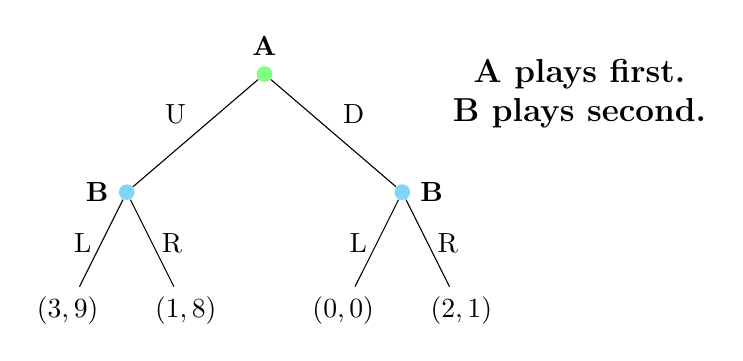
\begin{tikzpicture}[level distance=1.5cm,
  level 1/.style={sibling distance=3.5cm},
  level 2/.style={sibling distance=1.5cm}]
  \node[circle, fill=green!50, inner sep=2pt, label=above:\textbf{A}] {}
    child {node[circle, fill=cyan!50, inner sep=2pt, label=left:\textbf{B}] {}
      child {node {$(3,9)$} edge from parent node[left] {L}}
      child {node {$(1,8)$} edge from parent node[right] {R}}
      edge from parent node[above left] {U}
    }
    child {node[circle, fill=cyan!50, inner sep=2pt, label=right:\textbf{B}] {}
      child {node {$(0,0)$} edge from parent node[left] {L}}
      child {node {$(2,1)$} edge from parent node[right] {R}}
      edge from parent node[above right] {D}
    };
    \node at (4,0) {\large \textbf{A plays first.}};
    \node at (4,-0.5) {\large \textbf{B plays second.}};
\end{tikzpicture}
\end{center}

\subsection{Backward Induction}
To solve this, we reason backwards:
\begin{enumerate}
    \item \textbf{B's decision:}
    \begin{itemize}
        \item If A plays $U$, B chooses between $L$ (9) and $R$ (8). B chooses $L$. Payoff to A is 3.
        \item If A plays $D$, B chooses between $L$ (0) and $R$ (1). B chooses $R$. Payoff to A is 2.
    \end{itemize}
    \item \textbf{A's decision:} A knows B's optimal responses. A effectively chooses between the outcome of playing $U$ (which leads to $L$, giving A 3) and playing $D$ (which leads to $R$, giving A 2).
    \item Since $3 > 2$, A plays $U$.
\end{enumerate}

Thus, in the sequential version, $(U,L)$ is the likely Nash equilibrium.

\section{Mixed Strategies}

\subsection{Pure vs. Mixed Strategies}
Strategies like "Up", "Down", "Left", or "Right" are called \textbf{Pure Strategies}. Some games have no Nash equilibrium in pure strategies.

\begin{examplebox}{Matching Pennies / Competitive Game}
    Consider the following game:
    \begin{center}
    \renewcommand{\arraystretch}{1.5}
    \begin{tabular}{cc|c|c|}
      & \multicolumn{1}{c}{} & \multicolumn{2}{c}{\textbf{Player B}} \\
      & \multicolumn{1}{c}{} & \multicolumn{1}{c}{$L$}  & \multicolumn{1}{c}{$R$} \\ \cline{3-4}
      \multirow{2}*{\textbf{Player A}}  & $U$ & $(1,2)$ & $(0,4)$ \\ \cline{3-4}
      & $D$ & $(0,5)$ & $(3,2)$ \\ \cline{3-4}
    \end{tabular}
    \end{center}
    \textbf{Check for Pure NE:}
    \begin{itemize}
        \item $(U,L)$: B prefers $R$ ($4>2$). Not NE.
        \item $(U,R)$: A prefers $D$ ($3>0$). Not NE.
        \item $(D,R)$: B prefers $L$ ($5>2$). Not NE.
        \item $(D,L)$: A prefers $U$ ($1>0$). Not NE.
    \end{itemize}
    This game has \textbf{no pure strategy Nash equilibria}.
\end{examplebox}

However, a Nash equilibrium always exists if we allow for \textbf{Mixed Strategies}.
\begin{definition}[Mixed Strategy]
    A mixed strategy involves selecting a probability distribution over pure strategies.
    \begin{itemize}
        \item Player A plays $U$ with probability $\pi_U$ (or $p$) and $D$ with probability $1-\pi_U$.
        \item Player B plays $L$ with probability $\pi_L$ (or $q$) and $R$ with probability $1-\pi_L$.
    \end{itemize}
\end{definition}

\subsection{Calculating Mixed Strategy Equilibrium}

Let's compute the equilibrium for a standard example where pure strategies exist but we want to see the general method, or for games like the one above where only mixed strategies exist. Consider this generic payoff matrix:

\begin{center}
\renewcommand{\arraystretch}{1.5}
\begin{tabular}{cc|c|c|}
  & \multicolumn{1}{c}{} & \multicolumn{2}{c}{\textbf{Player B}} \\
  & \multicolumn{1}{c}{} & \multicolumn{1}{c}{$L$ ($q$)}  & \multicolumn{1}{c}{$R$ ($1-q$)} \\ \cline{3-4}
  \multirow{2}*{\textbf{Player A}}  & $U$ ($p$) & $(6,4)$ & $(3,5)$ \\ \cline{3-4}
  & $D$ ($1-p$) & $(4,3)$ & $(5,7)$ \\ \cline{3-4}
\end{tabular}
\end{center}

\subsubsection{Player A's Best Response}
We calculate Player A's \textbf{Expected Value (EV)} for playing purely $U$ or purely $D$, given B plays $L$ with probability $q$.
\begin{align*}
    EV^A(U) &= 6q + 3(1-q) = 3 + 3q \\
    EV^A(D) &= 4q + 5(1-q) = 5 - q
\end{align*}
Player A will choose $U$ if $EV^A(U) > EV^A(D)$:
\begin{align*}
    3 + 3q &> 5 - q \\
    4q &> 2 \implies q > 1/2
\end{align*}
Thus, A's best response strategy ($p$) is:
\begin{itemize}
    \item If $q > 1/2$, play $U$ ($p=1$).
    \item If $q < 1/2$, play $D$ ($p=0$).
    \item If $q = 1/2$, A is indifferent ($0 \le p \le 1$).
\end{itemize}

\subsubsection{Player B's Best Response}
Similarly, we calculate B's EV given A plays $U$ with probability $p$.
\begin{align*}
    EV^B(L) &= 4p + 3(1-p) = 3 + p \\
    EV^B(R) &= 5p + 7(1-p) = 7 - 2p
\end{align*}
Player B plays $L$ if $EV^B(L) > EV^B(R)$:
\begin{align*}
    3 + p &> 7 - 2p \\
    3p &> 4 \implies p > 4/3
\end{align*}
Since $p$ is a probability, it cannot exceed 1. Therefore, $3+p$ is \textbf{always less than} $7-2p$ (for valid range $0 \le p \le 1$). 
\begin{itemize}
    \item B's best response is always to play $R$ ($q=0$). $R$ is a strictly dominant strategy for B in this numerical example.
\end{itemize}

\subsubsection{Finding the Nash Equilibrium}
The Nash Equilibrium is the intersection of the best response curves.
\begin{itemize}
    \item A wants to match $q$.
    \item B always plays $q=0$.
    \item If $q=0$, A's best response is $D$ (since $q < 1/2$).
    \item Result: Pure strategy equilibrium $(D, R)$.
\end{itemize}

\subsection{Case with Multiple Equilibria (Hawk-Dove Game)}

Let's analyze a game of coexistence where mixed strategies are essential.
\begin{examplebox}{Hawk-Dove Game}
    Two animals (e.g., bears) contest a resource. They can be a \textbf{Hawk} (Aggressive) or a \textbf{Dove} (Passive).
    
    \begin{center}
    \renewcommand{\arraystretch}{1.5}
    \begin{tabular}{cc|c|c|}
      & \multicolumn{1}{c}{} & \multicolumn{2}{c}{\textbf{Bear 2}} \\
      & \multicolumn{1}{c}{} & \multicolumn{1}{c}{$H$ ($\pi_H^2$)}  & \multicolumn{1}{c}{$D$} \\ \cline{3-4}
      \multirow{2}*{\textbf{Bear 1}}  & $H$ ($\pi_H^1$) & $(-5,-5)$ & $(8,0)$ \\ \cline{3-4}
      & $D$ & $(0,8)$ & $(4,4)$ \\ \cline{3-4}
    \end{tabular}
    \end{center}
    
    \textbf{Pure Strategy Equilibria:}
    \begin{itemize}
        \item $(H,D)$ is a NE ($8>4$ for Bear 1, $0>-5$ for Bear 2).
        \item $(D,H)$ is a NE ($0>-5$ for Bear 1, $8>4$ for Bear 2).
        \item Note: $(D,D)$ is not a NE because a Hawk beats a Dove ($8>4$). $(H,H)$ is not a NE because fighting hurts both ($-5 < 0$).
    \end{itemize}
\end{examplebox}

\textbf{Mixed Strategy Equilibrium Calculation:}
Let $\pi_H^1$ be prob. Bear 1 is Hawk, $\pi_H^2$ be prob. Bear 2 is Hawk.

For Bear 1 to mix strategies, it must be indifferent between H and D:
\begin{align*}
    EV^1(H) &= -5\pi_H^2 + 8(1-\pi_H^2) = 8 - 13\pi_H^2 \\
    EV^1(D) &= 0\pi_H^2 + 4(1-\pi_H^2) = 4 - 4\pi_H^2
\end{align*}
Set $EV^1(H) = EV^1(D)$:
\begin{align*}
    8 - 13\pi_H^2 &= 4 - 4\pi_H^2 \\
    4 &= 9\pi_H^2 \\
    \pi_H^2 &= 4/9
\end{align*}
By symmetry, Bear 2 is indifferent when $\pi_H^1 = 4/9$.

\textbf{Best Response Dynamics:}
\begin{itemize}
    \item Bear 1 plays $H$ if $\pi_H^2 < 4/9$.
    \item Bear 1 plays $D$ if $\pi_H^2 > 4/9$.
\end{itemize}

This creates a reaction function plot where the two curves intersect at $(\pi_H^1, \pi_H^2) = (4/9, 4/9)$.

\begin{center}
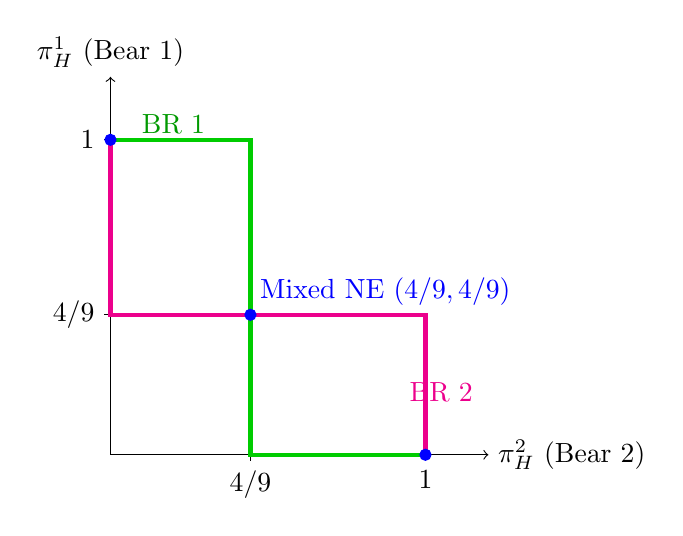
\begin{tikzpicture}[scale=4]
    % Axes
    \draw[->] (0,0) -- (1.2,0) node[right] {$\pi_H^2$ (Bear 2)};
    \draw[->] (0,0) -- (0,1.2) node[above] {$\pi_H^1$ (Bear 1)};
    
    % Ticks
    \draw (4/9, 0.02) -- (4/9, -0.02) node[below] {$4/9$};
    \draw (0.02, 4/9) -- (-0.02, 4/9) node[left] {$4/9$};
    \draw (1, 0.02) -- (1, -0.02) node[below] {$1$};
    \draw (0.02, 1) -- (-0.02, 1) node[left] {$1$};
    
    % Bear 1 Best Response (Green in slides) - Reaction to Bear 2 (x-axis)
    % If Bear 2 < 4/9, Bear 1 plays 1 (Hawk). If Bear 2 > 4/9, Bear 1 plays 0 (Dove).
    \draw[green!80!black, ultra thick] (0,1) -- (4/9,1) -- (4/9,0) -- (1,0);
    \node[green!60!black] at (0.2, 1.05) {BR 1};

    % Bear 2 Best Response (Pink in slides) - Reaction to Bear 1 (y-axis)
    % If Bear 1 < 4/9, Bear 2 plays 1 (Hawk). If Bear 1 > 4/9, Bear 2 plays 0 (Dove).
    \draw[magenta, ultra thick] (1,0) -- (1,4/9) -- (0,4/9) -- (0,1);
    \node[magenta] at (1.05, 0.2) {BR 2};
    
    % Intersections (Nash Equilibria)
    \filldraw[blue] (0,1) circle (0.5pt); % (D,H)
    \filldraw[blue] (1,0) circle (0.5pt); % (H,D)
    \filldraw[blue] (4/9,4/9) circle (0.5pt); % Mixed
    
    \node[above right, blue] at (4/9,4/9) {Mixed NE $(4/9, 4/9)$};
\end{tikzpicture}
\end{center}

\begin{remark}
There are three Nash equilibria in the Hawk-Dove game:
\begin{enumerate}
    \item Pure: Bear 1 is Hawk, Bear 2 is Dove.
    \item Pure: Bear 1 is Dove, Bear 2 is Hawk.
    \item Mixed: Each plays Hawk with probability $4/9$.
\end{enumerate}
\end{remark}

\section{Conclusion: Nash Existence Theorem}

We conclude with a fundamental theorem in Game Theory:
\begin{tcolorbox}[colback=blue!5!white,colframe=blue!75!black,title=Nash Existence Theorem]
    A game with a finite number of players, each with a finite number of pure strategies, has \textbf{at least one Nash equilibrium}.
\end{tcolorbox}
This implies that if a game has no pure strategy Nash equilibrium, it \textbf{must} have at least one mixed strategy Nash equilibrium.

\chapter{Exchange}

In the previous parts of the course, we have analyzed consumer theory and production theory separately. We are now entering Part 3: \textbf{General Equilibrium Theory}\index{General Equilibrium}. Unlike partial equilibrium analysis, which looks at a single market in isolation, general equilibrium analysis studies how demand and supply conditions interact in several markets to determine the prices of many goods.

We begin our study with the simplest form of general equilibrium: a pure \textbf{exchange economy}\index{Exchange Economy}. In this model, there is no production; economic agents trade their initial endowments of goods to achieve a more preferred allocation.

\section{The Edgeworth Box}

To analyze the exchange of goods between two consumers, Edgeworth and Bowley devised a diagrammatic tool known as the \textbf{Edgeworth Box}\index{Edgeworth Box}. This diagram allows us to depict the endowments, preferences, and possible allocations of two consumers simultaneously.

\subsection{Constructing the Box}
Consider an economy with two consumers, denoted by $A$ and $B$, and two goods, denoted by $1$ and $2$.
\begin{itemize}
    \item Let $\omega^A = (\omega_1^A, \omega_2^A)$ be consumer A's initial endowment.
    \item Let $\omega^B = (\omega_1^B, \omega_2^B)$ be consumer B's initial endowment.
\end{itemize}

The total quantity available of good 1 and good 2 in the economy is fixed by the sum of individual endowments:
\begin{align}
    \text{Total Good 1: } & \quad W_1 = \omega_1^A + \omega_1^B \\
    \text{Total Good 2: } & \quad W_2 = \omega_2^A + \omega_2^B
\end{align}

The Edgeworth box is a rectangle formed by these total quantities:
\begin{itemize}
    \item The \textbf{width} of the box represents the total amount of good 1 ($W_1$).
    \item The \textbf{height} of the box represents the total amount of good 2 ($W_2$).
\end{itemize}

\begin{remark}
    The origin for consumer A ($O_A$) is located at the bottom-left corner. Consumer A's consumption increases as we move to the right (for good 1) and upward (for good 2).
    
    The origin for consumer B ($O_B$) is located at the \textbf{top-right} corner. Crucially, consumer B's axes are reversed: his consumption of good 1 increases as we move to the \textit{left}, and his consumption of good 2 increases as we move \textit{down}.
\end{remark}

\subsection{Feasible Allocations}
An allocation is a specific distribution of goods between the consumers, denoted by $(x_1^A, x_2^A)$ for consumer A and $(x_1^B, x_2^B)$ for consumer B.

\begin{definition}[Feasible Allocation]\index{Feasible Allocation}
    An allocation is \textbf{feasible} if the total amount consumed equals the total amount available:
    \begin{align*}
        x_1^A + x_1^B &= \omega_1^A + \omega_1^B = W_1 \\
        x_2^A + x_2^B &= \omega_2^A + \omega_2^B = W_2
    \end{align*}
\end{definition}

Every point \textit{inside} or on the boundary of the Edgeworth box represents a feasible allocation. The initial \textbf{endowment allocation}\index{Endowment Allocation} is simply one specific point in this box, often marked as $\omega$.

\section{Preferences and Trade}

We can represent the preferences of both consumers by drawing their indifference curves inside the box.
\begin{itemize}
    \item \textbf{Consumer A's Indifference Curves:} Look like standard convex curves relative to $O_A$. Utility increases as curves move further away from $O_A$ (up and to the right).
    \item \textbf{Consumer B's Indifference Curves:} Are convex relative to $O_B$. Utility increases as curves move further away from $O_B$ (down and to the left).
\end{itemize}

\subsection{Pareto Improvement}
Starting from the endowment point $\omega$, consumers can trade. If consumer A gives up some good 1 in exchange for some good 2 from consumer B, they move to a new point in the box.

\begin{definition}[Pareto Improvement]\index{Pareto Improvement}
    An allocation is a \textbf{Pareto improvement} over the initial endowment if:
    \begin{enumerate}
        \item At least one consumer is strictly better off (higher utility), and
        \item The other consumer is strictly no worse off (utility is at least constant).
    \end{enumerate}
\end{definition}

Geometrically, the set of Pareto-improving allocations forms a "lens" shape bounded by the indifference curves of A and B passing through the initial endowment point. Trade will naturally occur within this lens because rational consumers will refuse any trade that lowers their utility.

\section{Pareto Efficiency}

As consumers continue to trade, they will eventually reach a point where no further Pareto improvements are possible.

\begin{definition}[Pareto Efficiency]\index{Pareto Efficiency}
    An allocation is \textbf{Pareto Efficient} (or Pareto Optimal) if there is no way to make one consumer better off without making the other consumer strictly worse off.
\end{definition}

\subsection{The Tangency Condition}
In the interior of the Edgeworth box, Pareto efficiency typically occurs where the indifference curves of the two consumers are \textbf{tangent} to each other.
\begin{itemize}
    \item If the curves intersect (cross each other), there is a "lens" area between them, indicating room for Pareto improvement.
    \item If they are tangent, their slopes are equal.
\end{itemize}

Since the slope of an indifference curve is the Marginal Rate of Substitution (MRS), the condition for Pareto efficiency is:
\begin{equation}
    MRS^A_{1,2} = MRS^B_{1,2}
\end{equation}
Intuitively, this means both consumers value the trade-off between good 1 and good 2 identically at the margin.

\section{The Contract Curve and The Core}

\subsection{The Contract Curve}
There are infinitely many Pareto efficient points in the box. If we connect all such points (all the points of tangency between A's and B's indifference curves), we trace out a line.

\begin{definition}[Contract Curve]\index{Contract Curve}
    The \textbf{Contract Curve} is the set of all Pareto-efficient allocations in the Edgeworth box.
\end{definition}

Note that the contract curve extends from consumer A's origin ($O_A$) to consumer B's origin ($O_B$). Being on the contract curve implies efficiency, but it does not say anything about equity or fairness.

\subsection{The Core}
While the contract curve represents all \textit{possible} efficient outcomes, rational consumers will only agree to trades that leave them at least as well off as they were with their initial endowments. They can always "block" a trade by simply refusing to participate and consuming their endowment.

\begin{definition}[The Core]\index{The Core}
    The \textbf{Core} of an exchange economy is the subset of the contract curve where allocations are Pareto-efficient \textit{and} constitute a welfare improvement (or at least no loss) for both consumers relative to their initial endowments.
\end{definition}

Geometrically, the Core is the segment of the Contract Curve that lies \textit{inside} the lens formed by the indifference curves passing through the endowment point $\omega$. We expect the outcome of rational bargaining or market trade to settle somewhere within the Core.
\chapter{Market Equilibrium and Welfare}

Previously, we determined that rational trade should lead to an allocation in the \textit{Core}. However, the Edgeworth box alone does not tell us exactly \textit{which} point in the Core will be reached. This depends on the trading mechanism. We now analyze the specific mechanism of \textbf{perfectly competitive markets}\index{Competitive Markets}.

\section{Trade in Competitive Markets}

Suppose there is a market mechanism where an "auctioneer" calls out prices $p_1$ and $p_2$ for good 1 and good 2. Consumers $A$ and $B$ are \textbf{price-takers}.

\subsection{The Budget Constraint}
Given prices $(p_1, p_2)$ and the initial endowment $\omega^i = (\omega_1^i, \omega_2^i)$, the value of a consumer $i$'s endowment determines their budget. The budget constraint is:
\begin{equation}
    p_1 x_1^i + p_2 x_2^i = p_1 \omega_1^i + p_2 \omega_2^i
\end{equation}
This line passes through the endowment point $\omega$. The slope of the budget line is $-\frac{p_1}{p_2}$.

\subsection{Optimal Choice}
Each consumer chooses the bundle $(x_1^{*i}, x_2^{*i})$ that maximizes their utility subject to this budget constraint. Geometrically, this occurs where the budget line is tangent to the highest attainable indifference curve.

We define the \textbf{Net Demand} (or Excess Demand) for consumer $i$ and good $j$ as:
\begin{equation}
    e_j^i = x_j^{*i} - \omega_j^i
\end{equation}
\begin{itemize}
    \item If $e_j^i > 0$, the consumer is a net buyer of good $j$.
    \item If $e_j^i < 0$, the consumer is a net seller of good $j$.
\end{itemize}

\section{General Equilibrium}

A general equilibrium requires that supply equals demand in all markets simultaneously.

\begin{definition}[Walrasian Equilibrium]\index{Walrasian Equilibrium}
    A price vector $(p_1^*, p_2^*)$ is a \textbf{General Equilibrium} if it causes both markets to clear:
    \begin{align}
        x_1^{*A} + x_1^{*B} &= \omega_1^A + \omega_1^B \quad (\text{Market for Good 1 clears}) \\
        x_2^{*A} + x_2^{*B} &= \omega_2^A + \omega_2^B \quad (\text{Market for Good 2 clears})
    \end{align}
\end{definition}

If markets do not clear (disequilibrium), prices will adjust. For instance, if there is excess demand for good 2, $p_2$ will rise relative to $p_1$, flattening the budget line until supply matches demand.

\section{Walras' Law}

Walras' Law is a fundamental identity in general equilibrium theory. It states that the value of aggregate excess demand is identically zero for \textit{any} set of prices, not just equilibrium prices.

\subsection{Derivation}
Consider the budget constraint for each consumer. Since preferences are well-behaved, consumers spend their entire income:
\begin{align}
    \text{Consumer A: } & p_1 x_1^{*A} + p_2 x_2^{*A} = p_1 \omega_1^A + p_2 \omega_2^A \\
    \text{Consumer B: } & p_1 x_1^{*B} + p_2 x_2^{*B} = p_1 \omega_1^B + p_2 \omega_2^B
\end{align}

Summing these equations gives the aggregate value of expenditure equals the aggregate value of endowments:
\begin{equation}
    p_1 (x_1^{*A} + x_1^{*B}) + p_2 (x_2^{*A} + x_2^{*B}) = p_1 (\omega_1^A + \omega_1^B) + p_2 (\omega_2^A + \omega_2^B)
\end{equation}

Rearranging terms to group by goods:
\begin{equation}
    p_1 \underbrace{(x_1^{*A} + x_1^{*B} - \omega_1^A - \omega_1^B)}_{z_1(p_1, p_2)} + p_2 \underbrace{(x_2^{*A} + x_2^{*B} - \omega_2^A - \omega_2^B)}_{z_2(p_1, p_2)} = 0
\end{equation}

Here, $z_1$ and $z_2$ represent the aggregate \textbf{excess demand functions} for good 1 and good 2. Thus, we arrive at Walras' Law:

\begin{proposition}[Walras' Law]\index{Walras' Law}
    For any positive prices $(p_1, p_2)$:
    \begin{equation}
        p_1 z_1(p_1, p_2) + p_2 z_2(p_1, p_2) \equiv 0
    \end{equation}
\end{proposition}

\subsection{Implications}
Walras' Law has powerful implications for finding equilibrium:
\begin{enumerate}
    \item \textbf{Market Redundancy:} If the market for good 1 is in equilibrium ($z_1 = 0$), then:
    \[ p_1(0) + p_2 z_2 = 0 \implies z_2 = 0 \]
    Therefore, if $n-1$ markets clear, the $n$-th market must also clear automatically.
    \item \textbf{Inverse Relationship:} An excess supply in one market ($z_1 < 0$) mathematically implies an excess demand in the other market ($z_2 > 0$) to keep the sum zero.
\end{enumerate}

\section{The Fundamental Theorems of Welfare Economics}

We conclude this chapter by linking the market mechanism back to the concept of Pareto Efficiency.

\subsection{The First Fundamental Theorem}
\begin{proposition}[First Welfare Theorem]\index{First Welfare Theorem}
    Given that consumers' preferences are well-behaved, any competitive equilibrium allocation is \textbf{Pareto Efficient}.
\end{proposition}

\textbf{Intuition:} In equilibrium, both consumers maximize utility subject to the \textit{same} prices. Thus:
\[ MRS^A = -\frac{p_1}{p_2} \quad \text{and} \quad MRS^B = -\frac{p_1}{p_2} \]
Since $MRS^A = MRS^B$, the tangency condition for Pareto efficiency is met. This theorem confirms Adam Smith's "Invisible Hand" hypothesis: separate agents pursuing self-interest leads to an efficient social outcome.

\subsection{The Second Fundamental Theorem}
The First Theorem deals with efficiency, but the outcome might be inequitable (e.g., Consumer A gets everything). Can we achieve a \textit{specific}, fair efficient outcome using markets?

\begin{proposition}[Second Welfare Theorem]\index{Second Welfare Theorem}
    Given well-behaved (convex) preferences, any Pareto Optimal allocation can be supported as a competitive equilibrium, provided the initial endowments are redistributed appropriately.
\end{proposition}

\textbf{Implication:} This theorem suggests a separation between \textit{efficiency} and \textit{distribution}. If society prefers a different efficient allocation (e.g., one that is more equal), it does not need to abandon the price mechanism. Instead, the government can transfer wealth (lump-sum transfers) to shift the endowment point $\omega$ to $\omega'$, and then let the market trade to the desired efficient point on the contract curve.

\begin{examplebox}{Summary of Key Concepts}
\begin{itemize}
    \item \textbf{Edgeworth Box:} Tool to analyze exchange.
    \item \textbf{Pareto Efficiency:} Cannot make someone better off without hurting another.
    \item \textbf{Contract Curve:} Locus of all Pareto efficient points.
    \item \textbf{Walras' Law:} Value of excess demands sums to zero.
    \item \textbf{First Welfare Theorem:} Markets $\to$ Efficiency.
    \item \textbf{Second Welfare Theorem:} Transfers + Markets $\to$ Any Efficient Outcome.
\end{itemize}
\end{examplebox}
\chapter{Externalities}

\section{Introduction}

In standard economic models, we typically assume that economic agents interact solely through markets and prices. However, in reality, the actions of one agent often directly affect the well-being of others outside of the market mechanism.

\begin{definition}[Externality]
An \textbf{externality} is a cost or a benefit imposed upon someone by actions taken by others. Crucially, the cost or benefit is generated \textit{externally} to that person; they are a third party who is not a participant in the activity that produces the effect.
\end{definition}

Externalities are classified based on their impact:
\begin{itemize}
    \item \textbf{Positive Externality:} An externally imposed benefit.
    \item \textbf{Negative Externality:} An externally imposed cost.
\end{itemize}

\begin{examplebox}{Examples of Externalities}
\textbf{Negative Externalities:}
\begin{itemize}
    \item \textbf{Air pollution:} A factory produces goods but pollutes the air, affecting the health of nearby residents.
    \item \textbf{Traffic congestion:} An additional car on the road slows down all other drivers.
    \item \textbf{Second-hand cigarette smoke:} A smoker enjoys their cigarette, but the smoke bothers or harms people nearby.
\end{itemize}

\textbf{Positive Externalities:}
\begin{itemize}
    \item \textbf{Property maintenance:} A well-maintained property increases the market value of neighboring properties.
    \item \textbf{Scientific advance:} Research and development can generate knowledge that benefits society beyond the specific firm that conducted the research.
    \item \textbf{Vaccination:} Getting vaccinated reduces the transmission of disease to others.
\end{itemize}
\end{examplebox}

\section{Inefficiency and The Consumption Model}

To understand why externalities lead to inefficiency, consider a simple model with two agents, A and B, and two commodities: Money ($m$) and Smoke ($s$).

\subsection{Preferences and Endowments}
\begin{itemize}
    \item \textbf{Agent A:} Likes both money and smoke. (Smoke might represent the pleasure of smoking or the output of a production process).
    \item \textbf{Agent B:} Likes money but dislikes smoke (Smoke is a ``bad'').
    \item \textbf{Endowments:} Agents are endowed with money $y_A$ and $y_B$. Smoke intensity is measured on a scale from $0$ to $1$.
\end{itemize}

\subsection{The Conflict}
If there is no mechanism to trade or negotiate regarding smoke:
\begin{enumerate}
    \item Agent A, preferring more smoke, will choose the maximum smoke level ($s=1$).
    \item Agent B, preferring less smoke, would prefer zero smoke ($s=0$).
\end{enumerate}

Typically, Agent A determines the smoke level (e.g., by lighting a cigarette). This creates an inefficient outcome. In an Edgeworth box-style analysis (adapted for a public good/bad), we can see that:
\begin{itemize}
    \item Agent A's most preferred choice ($s=1$) is inefficient because Agent B would be willing to pay A to reduce the smoke.
    \item Agent B's most preferred choice ($s=0$) is inefficient because Agent A would be willing to pay B to allow some smoke.
\end{itemize}

Efficient allocations are found where the marginal rate of substitution between money and smoke is equalized (tangency of indifference curves), or where the marginal benefit of smoke to A equals the marginal cost of smoke to B. Without a market for smoke, the economy fails to reach these efficient points.

\section{The Coase Theorem and Property Rights}

Ronald Coase provided a profound insight into the problem of externalities. He argued that most externality problems arise due to an \textbf{inadequate specification of property rights}. Because property rights over resources (like clean air) are undefined, markets cannot form to trade these rights.

\begin{definition}[Internalizing the Externality]
Causing a producer of an externality to bear the full external cost or to enjoy the full external benefit is called \textbf{internalizing the externality}.
\end{definition}

\subsection{Assigning Property Rights}
Let us revisit the Smoke vs. Money example. Suppose we create a property right for the air in the room and assign it to one of the agents.

\textbf{Case 1: Agent B owns the air.}
\begin{itemize}
    \item Agent B has the right to clean air ($s=0$).
    \item Agent B can sell ``rights to smoke'' to Agent A at a price $p(s_A)$.
    \item \textbf{Result:} Trade will occur. Agent A buys rights, and a positive amount of smoking ($s > 0$) occurs. Both agents are better off than at the no-smoke starting point. The equilibrium is Pareto efficient.
\end{itemize}

\textbf{Case 2: Agent A owns the air.}
\begin{itemize}
    \item Agent A has the right to smoke ($s=1$).
    \item Agent B can pay Agent A to \textit{reduce} smoke intensity.
    \item \textbf{Result:} Trade will occur. Agent B pays A to smoke less. The equilibrium is Pareto efficient.
\end{itemize}

\subsection{Quasilinear Preferences and The Coase Theorem}
A crucial question is whether the \textit{amount} of smoke generated depends on who owns the property rights.
\begin{itemize}
    \item Generally, the allocation of property rights affects the distribution of wealth (the owner gets richer). If preferences represent normal goods, wealth effects might change the demand for smoke.
    \item However, if preferences are \textbf{quasilinear} in money (i.e., $U(m, s) = m + f(s)$), there are no income effects on the demand for $s$.
\end{itemize}

\begin{proposition}[Coase Theorem]
If property rights are well-defined and trade is allowed (with zero transaction costs), the allocation of resources will be efficient. Furthermore, if preferences are quasilinear, the equilibrium level of the externality (e.g., amount of smoke) will be the same regardless of who is assigned the property right.
\end{proposition}

\section{Production Externalities: The Steel Mill and The Fishery}

We now formalize this using a production model involving two firms.
\begin{itemize}
    \item \textbf{Steel Mill ($S$):} Produces steel ($s$) and pollution ($x$).
    \item \textbf{Fishery ($F$):} Produces fish ($f$). Pollution ($x$) increases the cost of fishing.
\end{itemize}

\subsection{The Setup}
\begin{itemize}
    \item \textbf{Steel Firm Cost:} $c_S(s, x)$.
        \begin{itemize}
            \item Marginal cost of steel: $\frac{\partial c_S}{\partial s} > 0$.
            \item Pollution reduces production costs: $\frac{\partial c_S}{\partial x} \leq 0$. Conversely, reducing pollution raises costs.
        \end{itemize}
    \item \textbf{Fishery Cost:} $c_F(f, x)$.
        \begin{itemize}
            \item Pollution increases fishing costs: $\frac{\partial c_F}{\partial x} \geq 0$. This implies a \textbf{negative externality}.
        \end{itemize}
    \item Both firms are price takers with market prices $p_S$ and $p_F$.
\end{itemize}

\subsection{Private Optimization (Inefficient Outcome)}
If the Steel firm ignores the externality, it maximizes:
\[
\max_{s, x} \Pi_S = p_S s - c_S(s, x)
\]
The first-order conditions (FOCs) are:
\begin{align}
    p_S &= \frac{\partial c_S(s, x)}{\partial s} \quad \text{(Price = Marginal Production Cost)} \\
    0 &= -\frac{\partial c_S(s, x)}{\partial x} \quad \text{(Marginal Cost of Pollution Reduction = 0)}
\end{align}
The firm produces pollution until the marginal benefit of reducing cost is zero, ignoring the damage to the fishery.

\begin{examplebox}{Numerical Example: Independent Firms}
Suppose:
\begin{itemize}
    \item $p_S = 12$, $p_F = 10$.
    \item Steel Cost: $c_S(s, x) = s^2 + (x - 4)^2$.
    \item Fishery Cost: $c_F(f, x) = f^2 + xf$.
\end{itemize}

\textbf{Steel Firm's Choice:}
Max $\Pi_S = 12s - [s^2 + (x-4)^2]$.
FOCs:
\[ 12 - 2s = 0 \implies s^* = 6 \]
\[ -2(x - 4) = 0 \implies x^* = 4 \]
Max Profit: $\Pi_S = 12(6) - 36 - 0 = \$36$.

\textbf{Fishery's Choice (given $x=4$):}
Max $\Pi_F = 10f - [f^2 + 4f] = 6f - f^2$.
FOC: $6 - 2f = 0 \implies f^* = 3$.
Max Profit: $\Pi_F = 10(3) - [9 + 12] = 30 - 21 = \$9$.

\textbf{Total Industry Profit:} $\$36 + \$9 = \$45$.
\end{examplebox}

\subsection{Merger (Internalization)}
Suppose the two firms merge. The new firm internalizes the externality by maximizing joint profit:
\[
\max_{s, f, x} \Pi^m = p_S s - c_S(s, x) + p_F f - c_F(f, x)
\]
FOCs:
\begin{align}
    p_S &= \frac{\partial c_S}{\partial s} \\
    p_F &= \frac{\partial c_F}{\partial f} \\
    -\frac{\partial c_S}{\partial x} &= \frac{\partial c_F}{\partial x}
\end{align}
The third condition states: \textit{The marginal cost to the steel division of reducing pollution must equal the marginal benefit to the fishery division of less pollution.}

\begin{examplebox}{Numerical Example: Merger}
Using the same functions:
\[ \Pi^m = 12s - s^2 - (x-4)^2 + 10f - f^2 - xf \]
FOCs:
\begin{enumerate}
    \item Steel: $12 - 2s = 0 \implies s^m = 6$.
    \item Fish: $10 - 2f - x = 0$.
    \item Pollution: $-2(x-4) - f = 0 \implies f = -2(x-4)$.
\end{enumerate}
Substituting (3) into (2):
\[ 10 - 2[-2(x-4)] - x = 0 \]
\[ 10 + 4(x-4) - x = 0 \implies 10 + 4x - 16 - x = 0 \implies 3x = 6 \implies x^m = 2 \]
Then $f^m = -2(2-4) = 4$.

\textbf{Total Profit:}
$\Pi^m = (12 \times 6 - 36 - 4) + (10 \times 4 - 16 - 8) = 32 + 16 = \$48$.

\textbf{Conclusion:} Merger increases total profit ($48 > 45$) and reduces pollution ($2 < 4$). The outcome is efficient.
\end{examplebox}

\subsection{The Coase Solution: Market for Pollution}
What if they don't merge, but property rights are assigned? Suppose the Fishery owns the right to clean water. It sells ``rights to pollute'' to the Steel mill at price $p_x$.

\begin{itemize}
    \item \textbf{Fishery (Supplier of rights):} Maximizes $\Pi_F = p_f f - c_F(f, x) + p_x x$.
    \item \textbf{Steel Mill (Buyer of rights):} Maximizes $\Pi_S = p_S s - c_S(s, x) - p_x x$.
\end{itemize}

\textbf{Equilibrium:}
Efficiency requires the marginal damage to the fishery to equal the marginal savings to the steel firm, mediated by price $p_x$:
\[
\text{Marginal Benefit (Steel)} = -\frac{\partial c_S}{\partial x} = p_x = \frac{\partial c_F}{\partial x} = \text{Marginal Cost (Fishery)}
\]

Using the numerical example, the market clearing price $p_x$ will induce the Steel firm to choose $x=2$ and the Fishery to choose $f=4$. The resource allocation ($s, f, x$) is identical to the merger case. This confirms the Coase Theorem: assigning property rights creates a market that internalizes the externality.

\section{The Tragedy of the Commons}

This model explains the over-exploitation of resources owned in common (e.g., public grazing land, high-seas fisheries).

\subsection{The Model}
Consider a village grazing cows on a common pasture.
\begin{itemize}
    \item $c$: Number of cows.
    \item $f(c)$: Total milk production, where $f'(c) > 0$ and $f''(c) < 0$ (diminishing returns).
    \item $p_c$: Cost of grazing a cow.
    \item Price of milk = \$1.
\end{itemize}

\subsection{Efficient Allocation vs. Private Equilibrium}
\textbf{Social Optimum (Maximize Village Wealth):}
The village wants to maximize total profit:
\[ \max_{c} \Pi = f(c) - p_c c \]
FOC:
\[ f'(c^*) = p_c \]
The \textbf{Marginal Product} of the cow must equal the cost.

\textbf{Private Equilibrium (Tragedy):}
Since the land is common, villagers will enter (add cows) as long as it is profitable for them individually. An individual cares about the \textbf{Average Product}, not the marginal impact on others. Entry stops when profit per cow is zero:
\[ \frac{f(c)}{c} - p_c = 0 \implies \frac{f(c)}{c} = p_c \]
The \textbf{Average Product} of the cow equals the cost.

\subsection{Result}
Due to diminishing returns ($f'' < 0$), the Marginal Product is always less than the Average Product:
\[ f'(c) < \frac{f(c)}{c} \]
Since the private equilibrium equates Cost to Average Product, and the social optimum equates Cost to Marginal Product, the private equilibrium results in a larger number of cows:
\[ \hat{c} > c^* \]
The commons are over-grazed. The specific "tragedy" is that when a villager adds a cow, they get the average output, but they lower the average output for everyone else. They ignore this external cost inflicted on their neighbors.

\chapter{Asymmetric Information}
\label{chap:asymmetric_information}

In ideal competitive markets, we assume all agents have perfect information about the goods being traded. However, in the real world, information is often unevenly distributed.

\begin{definition}[Asymmetric Information]
\index{Asymmetric Information}
\textbf{Asymmetric information} occurs when one party in a transaction is in possession of more information than the other.
\end{definition}

This chapter explores how asymmetric information affects the functioning of a market, leading to phenomena such as adverse selection, signaling, and moral hazard.

% =========================================================================
% Section 1: Adverse Selection
% =========================================================================
\section{Adverse Selection}
\index{Adverse Selection}

Adverse selection creates a problem where "bad" products or customers are more likely to be selected in a market transaction due to hidden information. This phenomenon is famously illustrated by the market for used cars.

\subsection{The Market for Lemons}
Consider a market for used cars (often called "lemons" if they are bad quality).

\begin{examplebox}{The Used-Car Market Model}
\textbf{Assumptions:}
\begin{itemize}
    \item Car quality is uniformly distributed between \$1,000 and \$2,000.
    \item Sellers know the true quality (value) of their cars.
    \item Buyers are unaware of the true value of any specific car.
    \item \textbf{Valuation:} If a seller values a car at $X$, a buyer values it at $X + \$300$.
\end{itemize}

\textbf{Analysis of Trade:}
If there were perfect information, every car would be traded because the buyer values the car \$300 more than the seller. Gains from trade would be realized for all cars.

However, under asymmetric information, buyers only know the distribution.
\begin{enumerate}
    \item \textbf{Initial Expectation:} The average value of cars on the market (from \$1,000 to \$2,000) is \$1,500.
    \item \textbf{Buyer's Willingness to Pay:} The expected value to a buyer is:
    \[
    E[\text{Value}_{buyer}] = \$1,500 + \$300 = \$1,800
    \]
    \item \textbf{Market Unraveling:} If the market price is \$1,800, sellers who value their cars \textit{above} \$1,800 (high-quality cars) will exit the market.
    \item \textbf{Second Iteration:} Now, only cars with seller values between \$1,000 and \$1,800 remain. The new average seller value is \$1,400.
    \item \textbf{New Price:} The buyer's new expected value is:
    \[
    \$1,400 + \$300 = \$1,700
    \]
    Sellers with cars valued between \$1,700 and \$1,800 now exit.
\end{enumerate}

\textbf{Equilibrium:}
The market continues to shrink until an equilibrium is reached where the price buyers are willing to pay matches the marginal seller's valuation. Let $v_H$ be the value of the highest-quality car remaining in the market. The distribution is $[1000, v_H]$.
\[
\text{Price} = \underbrace{\left( \frac{1000 + v_H}{2} \right)}_{\text{Avg Seller Value}} + 300
\]
For the marginal seller ($v_H$) to stay, Price must equal $v_H$:
\[
\frac{1000 + v_H}{2} + 300 = v_H \implies 800 + 0.5 v_H = v_H \implies v_H = 1,600
\]
\textbf{Result:} In equilibrium, only cars valued by sellers between \$1,000 and \$1,600 are traded. Cars valued between \$1,600 and \$2,000 are driven out of the market, resulting in a deadweight loss.
\end{examplebox}

\subsection{Adverse Selection with Quality Choice}
Adverse selection can be severe enough to destroy a market entirely, especially when producers choose the quality level.

\begin{examplebox}{The Shoe Market}
Consider a market with two types of shoes: \textbf{High-quality} and \textbf{Low-quality}.
\begin{itemize}
    \item \textbf{Buyer Valuation:} High: \$14, Low: \$8. (Buyers cannot distinguish quality before purchase).
    \item \textbf{Marginal Cost:} High: \$11, Low: \$10.
\end{itemize}

\textbf{Scenario Analysis:}
\begin{enumerate}
    \item \textbf{High-Quality Only Equilibrium?}
    Suppose all sellers make high-quality shoes. Buyers pay \$14. Profit is $\$14 - \$11 = \$3$.
    However, a seller could deviate and make low-quality shoes (cost \$10). Buyers effectively pay \$14 (since they expect high quality), yielding a profit of $\$14 - \$10 = \$4$.
    Since deviation is profitable ($4 > 3$), this equilibrium cannot hold.

    \item \textbf{Low-Quality Only Equilibrium?}
    Suppose all sellers make low-quality shoes. Buyers realize this and pay \$8.
    Cost is \$10. Sellers incur a loss ($\$8 - \$10 = -\$2$). No trade occurs.

    \item \textbf{Pooling Equilibrium?}
    Suppose a fraction $q$ of sellers make high-quality shoes ($0 < q < 1$).
    Buyer's Expected Value (EV):
    \[
    EV = 14q + 8(1-q) = 8 + 6q
    \]
    For high-quality sellers to participate, Price ($EV$) must cover Cost (\$11):
    \[
    8 + 6q \ge 11 \implies 6q \ge 3 \implies q \ge 1/2
    \]
    At least 50\% of sellers must be high-quality. However, even if $q \ge 1/2$, a high-quality seller still gains \$1 extra profit by switching to low quality (Cost drops from \$11 to \$10).
\end{enumerate}

\textbf{Conclusion:} The proportion of high-quality sellers $q$ will decrease towards zero. Once $q$ is low, buyers pay only \$8, which covers no one's cost. \textbf{The market collapses completely.}
\end{examplebox}

\begin{remark}[Gresham's Law]
The phenomenon where "bad money drives out good" is applicable here. Low-quality goods drive high-quality goods out of the market, potentially leading to a total cessation of trade.
\end{remark}

% =========================================================================
% Section 2: Signaling
% =========================================================================
\section{Signaling}
\index{Signaling}

Adverse selection arises from information deficiency. \textbf{Signaling} allows the informed party (e.g., the seller or worker) to credibly convey private information to the uninformed party.

\subsection{Mechanisms}
\begin{itemize}
    \item \textbf{Warranties:} A high-quality seller offers a strong warranty (e.g., "replacement without repair"). This is costly for low-quality sellers to mimic, making the signal credible.
    \item \textbf{Education:} In the labor market, high-ability workers acquire education to signal their productivity.
\end{itemize}

\subsection{The Educational Signaling Model}
Consider a labor market with two types of workers:
\begin{itemize}
    \item \textbf{High-ability ($H$):} Marginal Product $a_H$. Fraction of population $h$.
    \item \textbf{Low-ability ($L$):} Marginal Product $a_L$. Fraction $1-h$.
    \item Note: $a_L < a_H$.
\end{itemize}

If firms cannot distinguish types, they pay the \textbf{pooling wage} equal to the expected marginal product:
\[
w_P = (1-h)a_L + h a_H
\]
Since $w_P < a_H$, high-ability workers are underpaid and have an incentive to signal their type.

\subsubsection{Cost of Signaling}
Workers can acquire education level $e$. Assume education does \textbf{not} increase productivity (it is a pure signal), but it is costly.
\begin{itemize}
    \item Cost for High-ability: $c_H$ per unit.
    \item Cost for Low-ability: $c_L$ per unit.
    \item \textbf{Crucial Assumption:} $c_L > c_H$ (Education is more "painful" or costly for low-ability workers).
\end{itemize}

\subsubsection{Separating Equilibrium}
In a separating equilibrium, high-ability workers acquire education $e_H$ and are paid $w_H = a_H$, while low-ability workers choose $e=0$ and are paid $w_L = a_L$.

For this to be an equilibrium, two self-selection constraints must be satisfied:

\begin{enumerate}
    \item \textbf{Participation constraint for High-ability:}
    The net benefit of acquiring education and getting the high wage must exceed the benefit of acting like a low type.
    \[
    w_H - c_H e_H > w_L \implies a_H - a_L > c_H e_H
    \]
    \item \textbf{Incentive compatibility for Low-ability:}
    The low-ability worker must prefer the low wage with no education over the high wage with the high education cost.
    \[
    w_L > w_H - c_L e_H \implies c_L e_H > a_H - a_L
    \]
\end{enumerate}

Combining these inequalities, a credible signal $e_H$ must satisfy:
\begin{equation}
\frac{a_H - a_L}{c_L} < e_H < \frac{a_H - a_L}{c_H}
\end{equation}

\begin{remark}[Inefficiency of Signaling]
Although signaling solves the information asymmetry (allowing firms to distinguish types), it generates a \textbf{deadweight loss}. Resources are spent on education ($c_H e_H$) that does not increase total output ($a_H$ and $a_L$ remain unchanged). The information is improved, but the gains from trade may not necessarily increase.
\end{remark}

% =========================================================================
% Section 3: Moral Hazard
% =========================================================================
\section{Moral Hazard}
\index{Moral Hazard}

While adverse selection concerns hidden information \textit{before} a transaction, \textbf{moral hazard} concerns hidden actions \textit{after} the transaction.

\begin{definition}[Moral Hazard]
Moral hazard is a reaction to incentives to increase the risk of a loss, resulting from asymmetric information regarding the agent's behavior.
\end{definition}

\begin{example}
\textbf{Car Insurance:} If an individual has full car insurance, they have less incentive to lock their car or park in safe locations. The probability of theft increases because the insurer cannot perfectly monitor the driver's actions.
\end{example}

\subsection{Market Implications}
If insurers cannot distinguish behavior (or risk types) perfectly:
\begin{itemize}
    \item They must offer a single contract to all insurees.
    \item High-risk and low-risk types are pooled.
    \item Low-risk individuals effectively subsidize high-risk individuals.
    \item This can lead to premiums rising so high that low-risk people drop out (similar to adverse selection), potentially causing market failure.
\end{itemize}


% ... 继续添加

\backmatter%
\addcontentsline{toc}{chapter}{Index}
\printindex

\end{document}
